\chapter{Ergebnisse}
    Innerhalb diese Kapitels geht es zunächst um die Vorbereitung der Proben.
    Weiter geht es es um den Umgang mit dem dreidimensionalen Datensatz sowie dessen Bearbeitung.
    Die verschiedenen extrahierten Darstellungen werden dann aufgenommen und analysiert.
    In dieser Arbeit untersuchten Gold und Nickeloxid Proben wurden alle in dem Versuchsaufbau aus \autoref{sec:Versuchsaufbau} vorbereitet und vermessen.
    Die Eisenoxid Proben wurden an der NanoESCA Beamline am Synchrotron Elettra in Triest präperiert und charakterisiert \footnote{Näheres zu diesem Versuchsaufbau und der Behandlung der Daten kann in \cite{ma-DJ} gefunden werden.}.

    \section{Vorbereitung und Präperation}
        \label{sec:Praep}
        \begin{itemize}
            \item IV Kurven? NiO und Gold
        \end{itemize}
            \begin{figure}
                \centering
                \begin{subfigure}{0.48\textwidth}
                    \centering
                    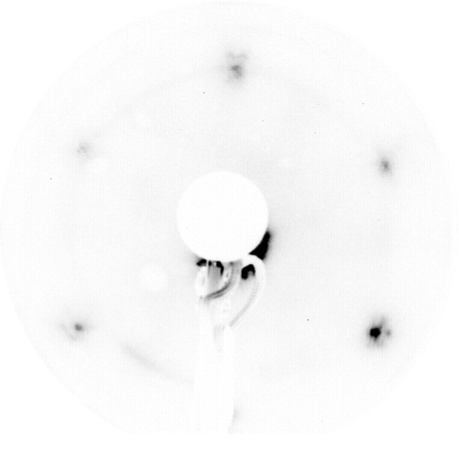
\includegraphics[height=5cm]{./content/pictures/2021_06_08_002_Au(111)_75eV}
                    \subcaption{Gold (111) bei einer Elektronenenergie von \SI{75}{\electronvolt}.}
                    \label{fig:LEED_Au}
                \end{subfigure}
                \begin{subfigure}{0.48\textwidth}
                    \centering
                    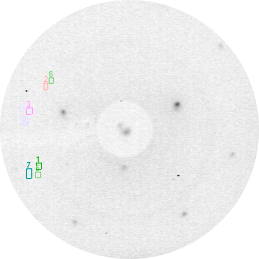
\includegraphics[height=5cm]{./content/pictures/FeO/2021_09_07_002_passivatedFe(100)_125eV.png}
                    \subcaption{Passiviertes Eisen (100) bei einer Elektronenenergie von \SI{125}{\electronvolt}.}
                    \label{fig:LEED_pFe}
                \end{subfigure}
                \caption{Die LEED-Bilder für die sauberen Substrate.}
            \label{fig:Substrate}
            \end{figure}
            Zum Präperieren der Proben werden zunächst die verschiedenen Substrate durch mehrfaches ioneninduziertes Zerstäuben und aufheizen gereinigt.
            Für die Goldprobe wurde eine Spannung von \SI{2}{\kilo\volt} und ein Strom von \SI{10}{\milli\ampere}, mit anschließendenem Aufheizen auf etwa \SI{500}{\celsius} verwendet.
            Anschließend wird die Oberflächenstruktur mittels LEED überprüft, dabei ergibt sich das Bild in \autoref{fig:Substrate}.
            Es ist sind scharfe Spots zu erkennen, ebenso wie die charakteristische kleineren Spots um die Hauptspots, die von der Fischgräten-Rekonstruktion herrühren.
            Die unterschiedlichen Intensität der einzelnen Reflexe rühr ebenfalls von der Rekonstruktion her.

            Hingegen wurde bei der Eisenprobe nur ein Spannung von \SI{1}{\kilo\volt} gewählt um die Probe zu reinigen, da es sich um einen dünnen auf Magnesiumoxid gewachsenen Film handelt.
            Allerdings wurde die Probe dann auf etwa \SI{600}{\celsius} aufgeheizt.
            Um Verunreinigungen des sehr reaktiven sauberen Eisens zu vermeiden, wird die Probe anschließend direkt passiviert.
            Dies geschieht in einer Sauerstoffatmosphäre von \SI{1.3e-7}{\milli\bar} für fünf Minuten, während die Probe bei \SI{550}{\celsius} gehalten wird.
            Die Probe wird dann nocheinmal kurz auf \SI{600}{\celsius} aufgeheizt.
            Nun wird auch dessen Oberflächenbeschaffenheit kontrolliert und entsprechendes LEED-Bild ist in \autoref{fig:LEED_pFe} zu sehen.
            Sie Spots sind scharf und zeigen auch die Geometrie der Fe-p$(1 \times 1)$O Struktur.
            Die gesamten Spots sind dabei nicht zentrosymmetrisch, da die Probe verkippt ist, wodurch auch der (0,0)-Reflex zu sehen ist.
            
            \begin{figure}
                \centering
                \begin{subfigure}{0.48\textwidth}
                    \centering
                    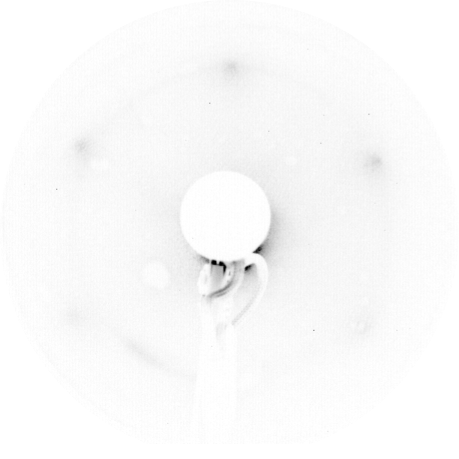
\includegraphics[height=5cm]{./content/pictures/2021_06_15_019_NiO(111)_73eV_Thicklayer}
                    \subcaption{Der Nickeloxidfilm (111) bei einer Elektronenenergie von \SI{73}{\electronvolt}.}
                \end{subfigure}
                \begin{subfigure}{0.48\textwidth}
                    \centering
                    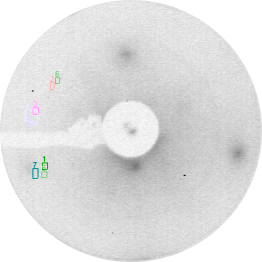
\includegraphics[height=5cm]{./content/pictures/FeO/2021_09_09_001_FeO_125eV.png}
                    \subcaption{Eisenoxid (100) bei der Elektronenenergie von \SI{125}{\electronvolt}.}
                \end{subfigure}
                \caption{Bilder der Beugung niederenergetischer Elektronen für die gewachsenen Filme.}
            \label{fig:Filme}
            \end{figure}
            Nun wurde auf die Goldprobe bei Raumtemperatur ein Nickeloxidfilm aufgebracht, dies geschieht durch das Aufdampfen von Nickel mit einer Rate von \SI{0.3}{\angstrom\per\minute} in einer Sauerstoffatmosphäre von \SI{2e-6}{\milli\bar}.
            Für den Eisenoxidfilm wird Eisen mit einer Rate von \SI{0.6}{\ML\per\minute} und einem Sauerstoffdruck von \SI{2e-7}{\milli\bar} auf die passivierte Eisenoberfläche aufgedampft.
            Dabei wird die Probe auf eine Temperatur von \SI{230}{\celsius} gehalten und anschließend bei \SI{650}{\celsius} ausgeheizt.
            Beide Filme werden erneut mittels LEED überprüft, das Eisenoxid zusätzlich mittels Augerelektronenspektroskopie.
            Die entsprechenden LEED-Bilder sind in \autoref{fig:Filme} dargestellt.

            Bei dem Nickeloxidfilm wie auch dem Eisenoxidfilm fällt auf, dass im Gegensatz zur Goldprobe die Spots eher ausgewaschen scheinen.
            Die Positionen der Punkte hat sich bei dem Nickeloxidfilm im Vergleich zum Gold nicht wesentlich verändert.
            Auch die Intensitäten der Reflexe ist nun gleich groß für alle Punkte.
            Hingegen sind beim Eisenoxid die Intensitäten invertiert, wobei die zuvor straken Spots nicht mehr sichtbar sind.
            Trotz der gleichen Elektronenenergie von \SI{125}{\electronvolt} sind die Spots leicht nach außen gewandert.
            Dies Widerspricht sich mit der eigentlich größeren Gitterkonstante von Eisenoxid im Bezug auf die p$(1 \times 1)$O Überstruktur des passivierten Eisens.

            Anschließend werden die beiden nun antiferromagnnetischen Substrate vermessen und anschließend wird eine Monolage Pentacene aufgedampft.
            Nach dem Aufdampfen wurde versucht LEED-Bilder aufzunehmen, es waren allerdings nur leichte Substratspots sichtbar.
            So lässt sich schlussfolgern, dass sich die Moleküle auf der Oberfläche nicht anordnen.

            \begin{figure}
                \centering
                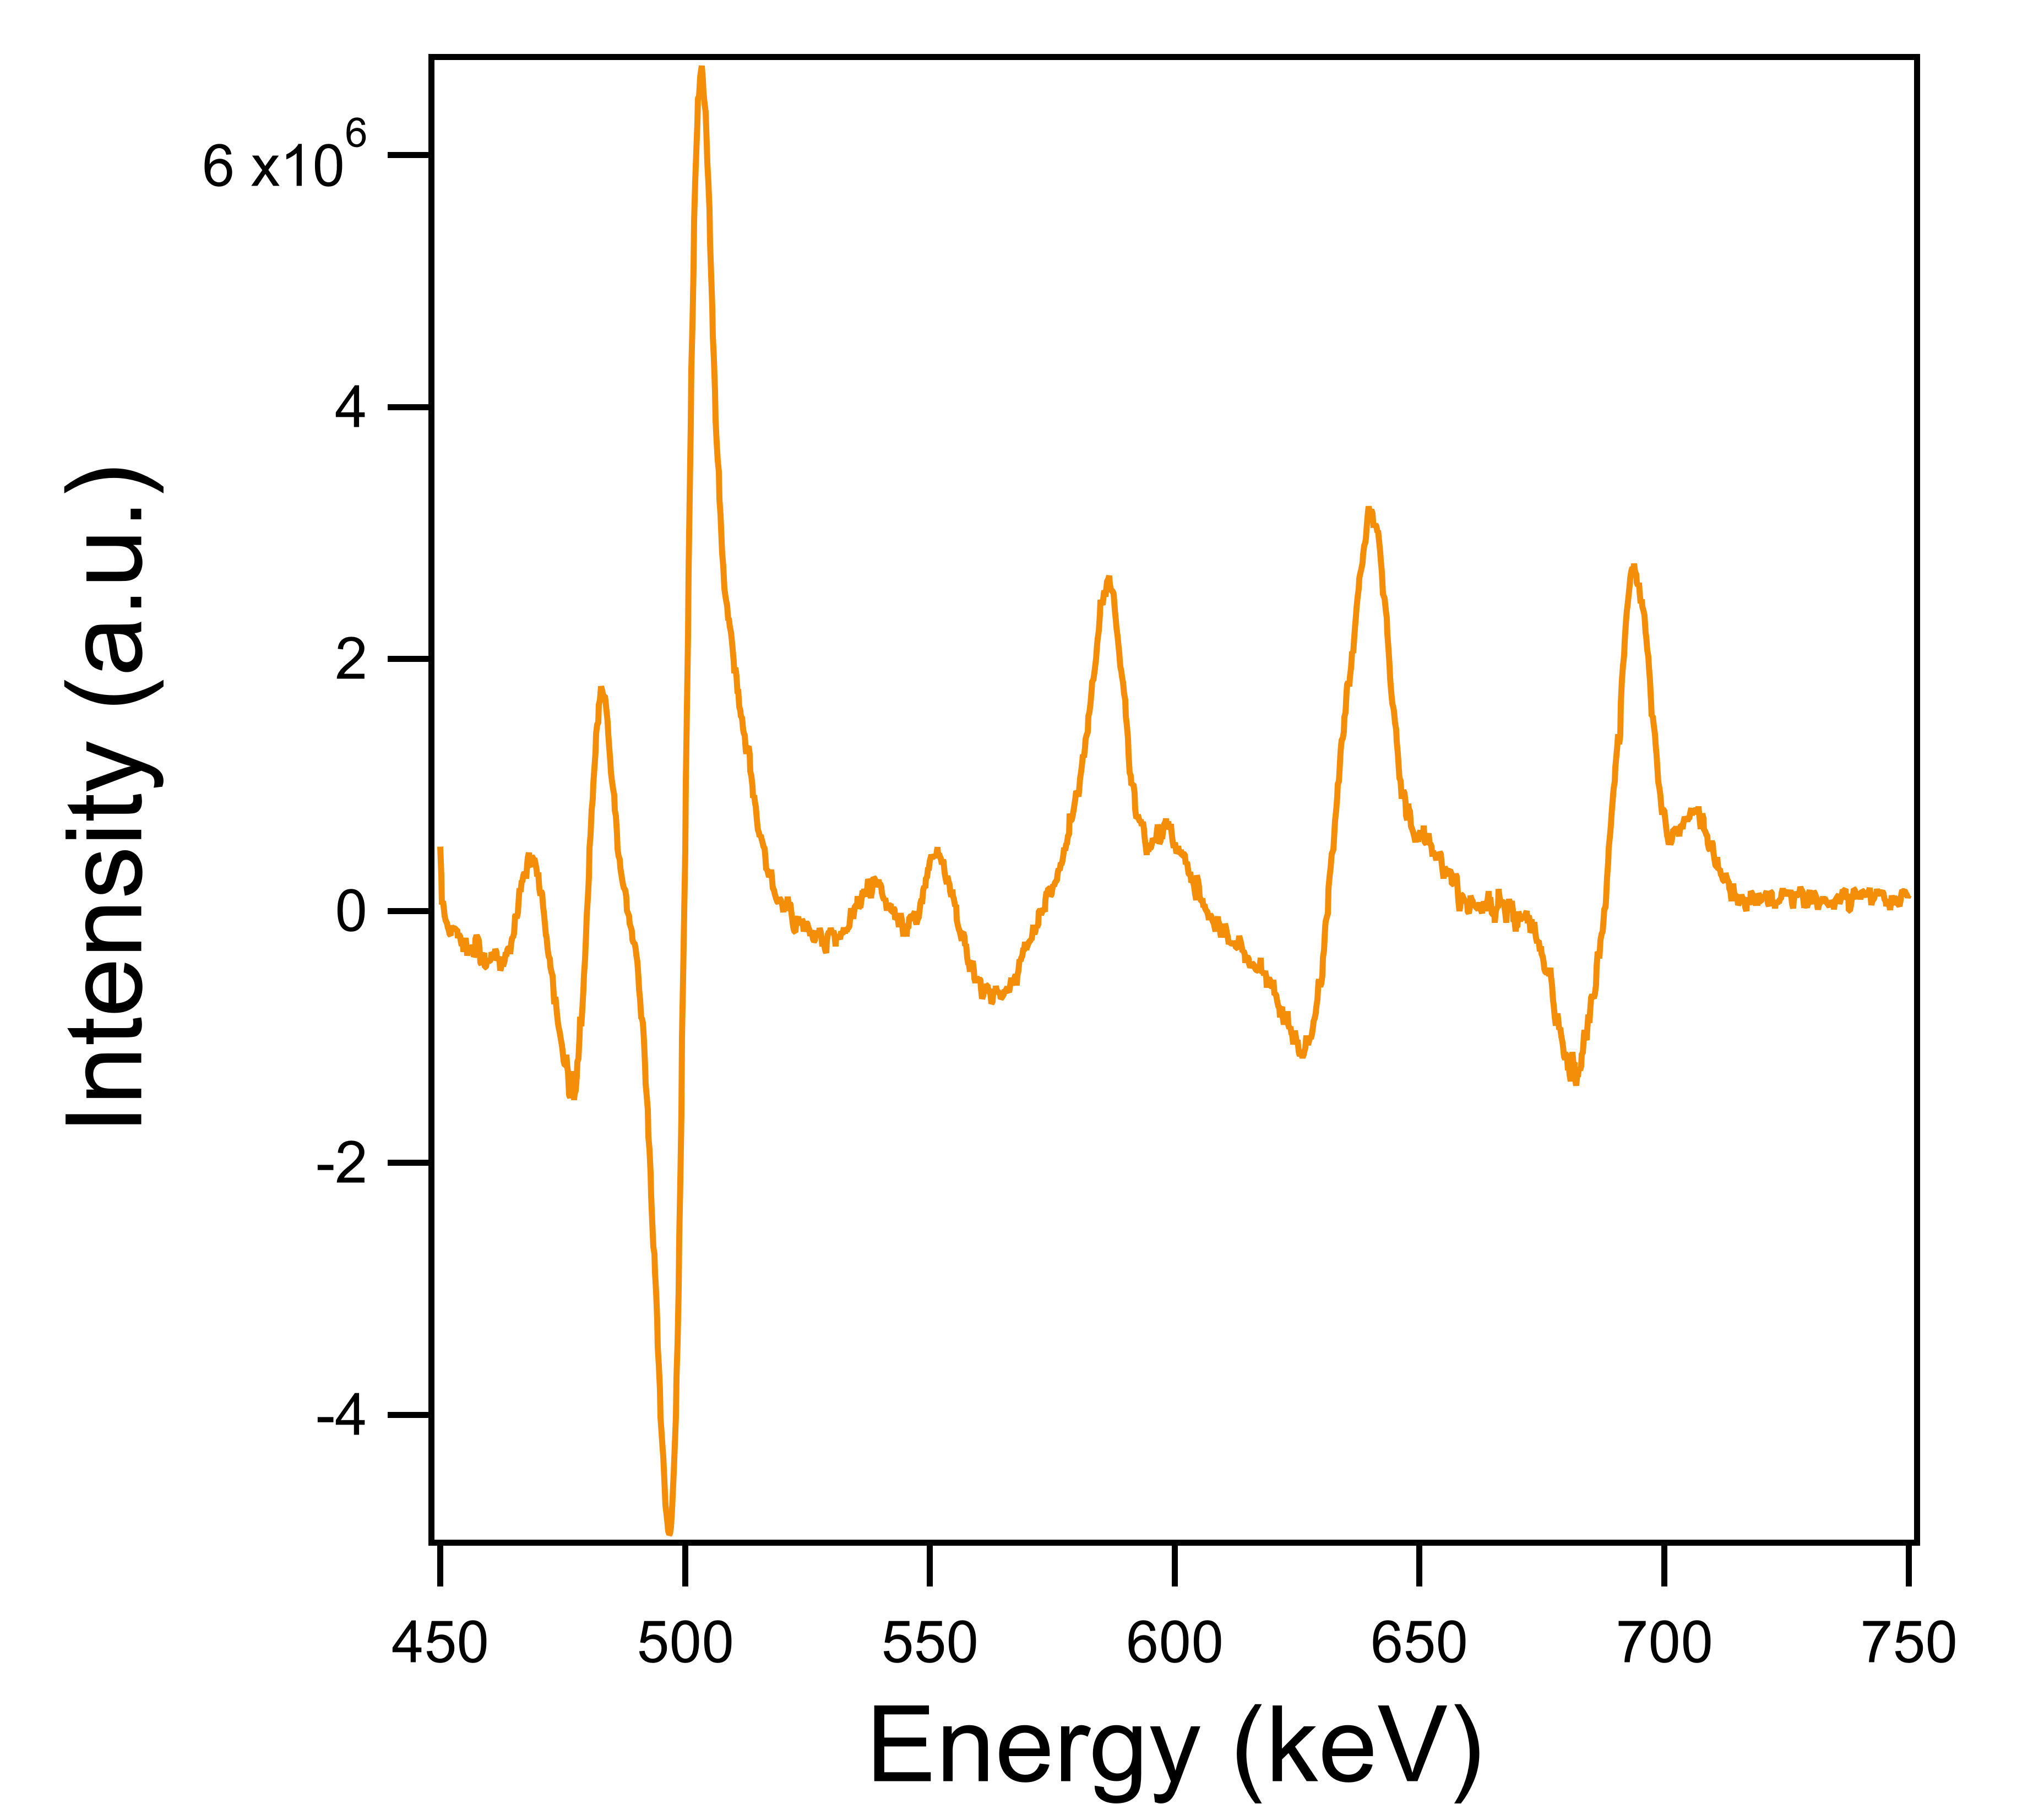
\includegraphics[width=0.6\textwidth]{./content/pictures/FeO/2021_09_09_001_AES_FeO.png}
                \caption{Das Augerspektrum für den Eisenoxidfilm.}
                \label{fig:Auger}
            \end{figure}
            Auch das Augerspektrum in \autoref{fig:Auger} mit dem bereits von Carpa u.A. \cite{FeO_1} entdecken Augerelektronenspektrum für Eisenoxid zeigt gute Übereinstimmung.
            Ebenfalls deutet das Peakverhältnis von dem Sauerstoffsignal bei \SI{503}{\electronvolt} und dem Signal für Eisen bei \SI{651}{\electronvolt} mit \num{2.53} auf $\ce{FeO}$ hin \cite{FeO_1, Auger}.
        

    \section{Datenformat und Bearbeitung}
    \begin{itemize}
        \item Kreios vorgehen
        \item NanoESCA vorgehen
    \end{itemize}
        Für die Auswertung der dreidimensionalen Datenwird die Software IGOR Pro \cite{IGOR} genutzt.
        Alle Messungen der winkelaufgelösten Bandstruktur wurden als dreidimensionale Datensätze aufgenommen.
        Da die Bilder auf Grund nicht perfekt eingestellter Linsen nicht kreisrund sind, werden die Elipsen angepasst.
        Hierfür wird die kleiner der beiden Achsen entlang der Achse gestreckt.
        Ferner muss der Polarisationsfaktor unter Beachtung der Substratgeometrie kompensiert werden.
        Hierfür werden die Bilder jeweils um \SI{\pm120}{} gedreht und auf das ursprüngliche Bild aufaddiert.
        Um die gemessene kinetische Energie in die relevante Bindungsenergie umzurechnen wird bei den integrierten Spektren aus \autoref{sec:EDC} eine Faltung aus \textbf{...} an die Fermikante durchgeführt.
        Zusätzlich müssen die gemessenen Bilder von ihren Pixelwerten noch in die entsprechenden Impulswerte umgerechnet werden.
        Dies geschieht mit Hilfe der Sekundärelektronen aus dem Spektrum der Austrittsarbeit (niedrige kinetische Energie).
        Ihre kinetische Energie kann durch 
        \begin{equation}
            E_\text{Kin} = \frac{\hbar^2 {k_{||}}^2}{2 m}
            \label{eqn:WKF}
        \end{equation}
        beschrieben werden, wobei $m$ die Elektronenmasse und $k_{||}$ ihr Impuls parallel zur Oberfläche ist.
        Die langsamsten Elektronen treten mit einer kinetischen Energie von \SI{0}{\electronvolt} aus der Probe aus und bilden damit den unteren Punkt der Parabel in \autoref{fig:WKF}.
        Durch ihren parabolischen Verlauf kann nun bei einer höher liegenden Energie ein Linienprofil genommen werden.
        Da sich die Elektronen wie in \autoref{eqn:WKF} verhalten können damit die Pixel in entsprechende Impulswerte umgerechnet werden.


    \section{Integrierte Spektren}
    \label{sec:EDC}
        % \begin{wrapfigure}{r}{5cm}
        \begin{figure}
            \centering
            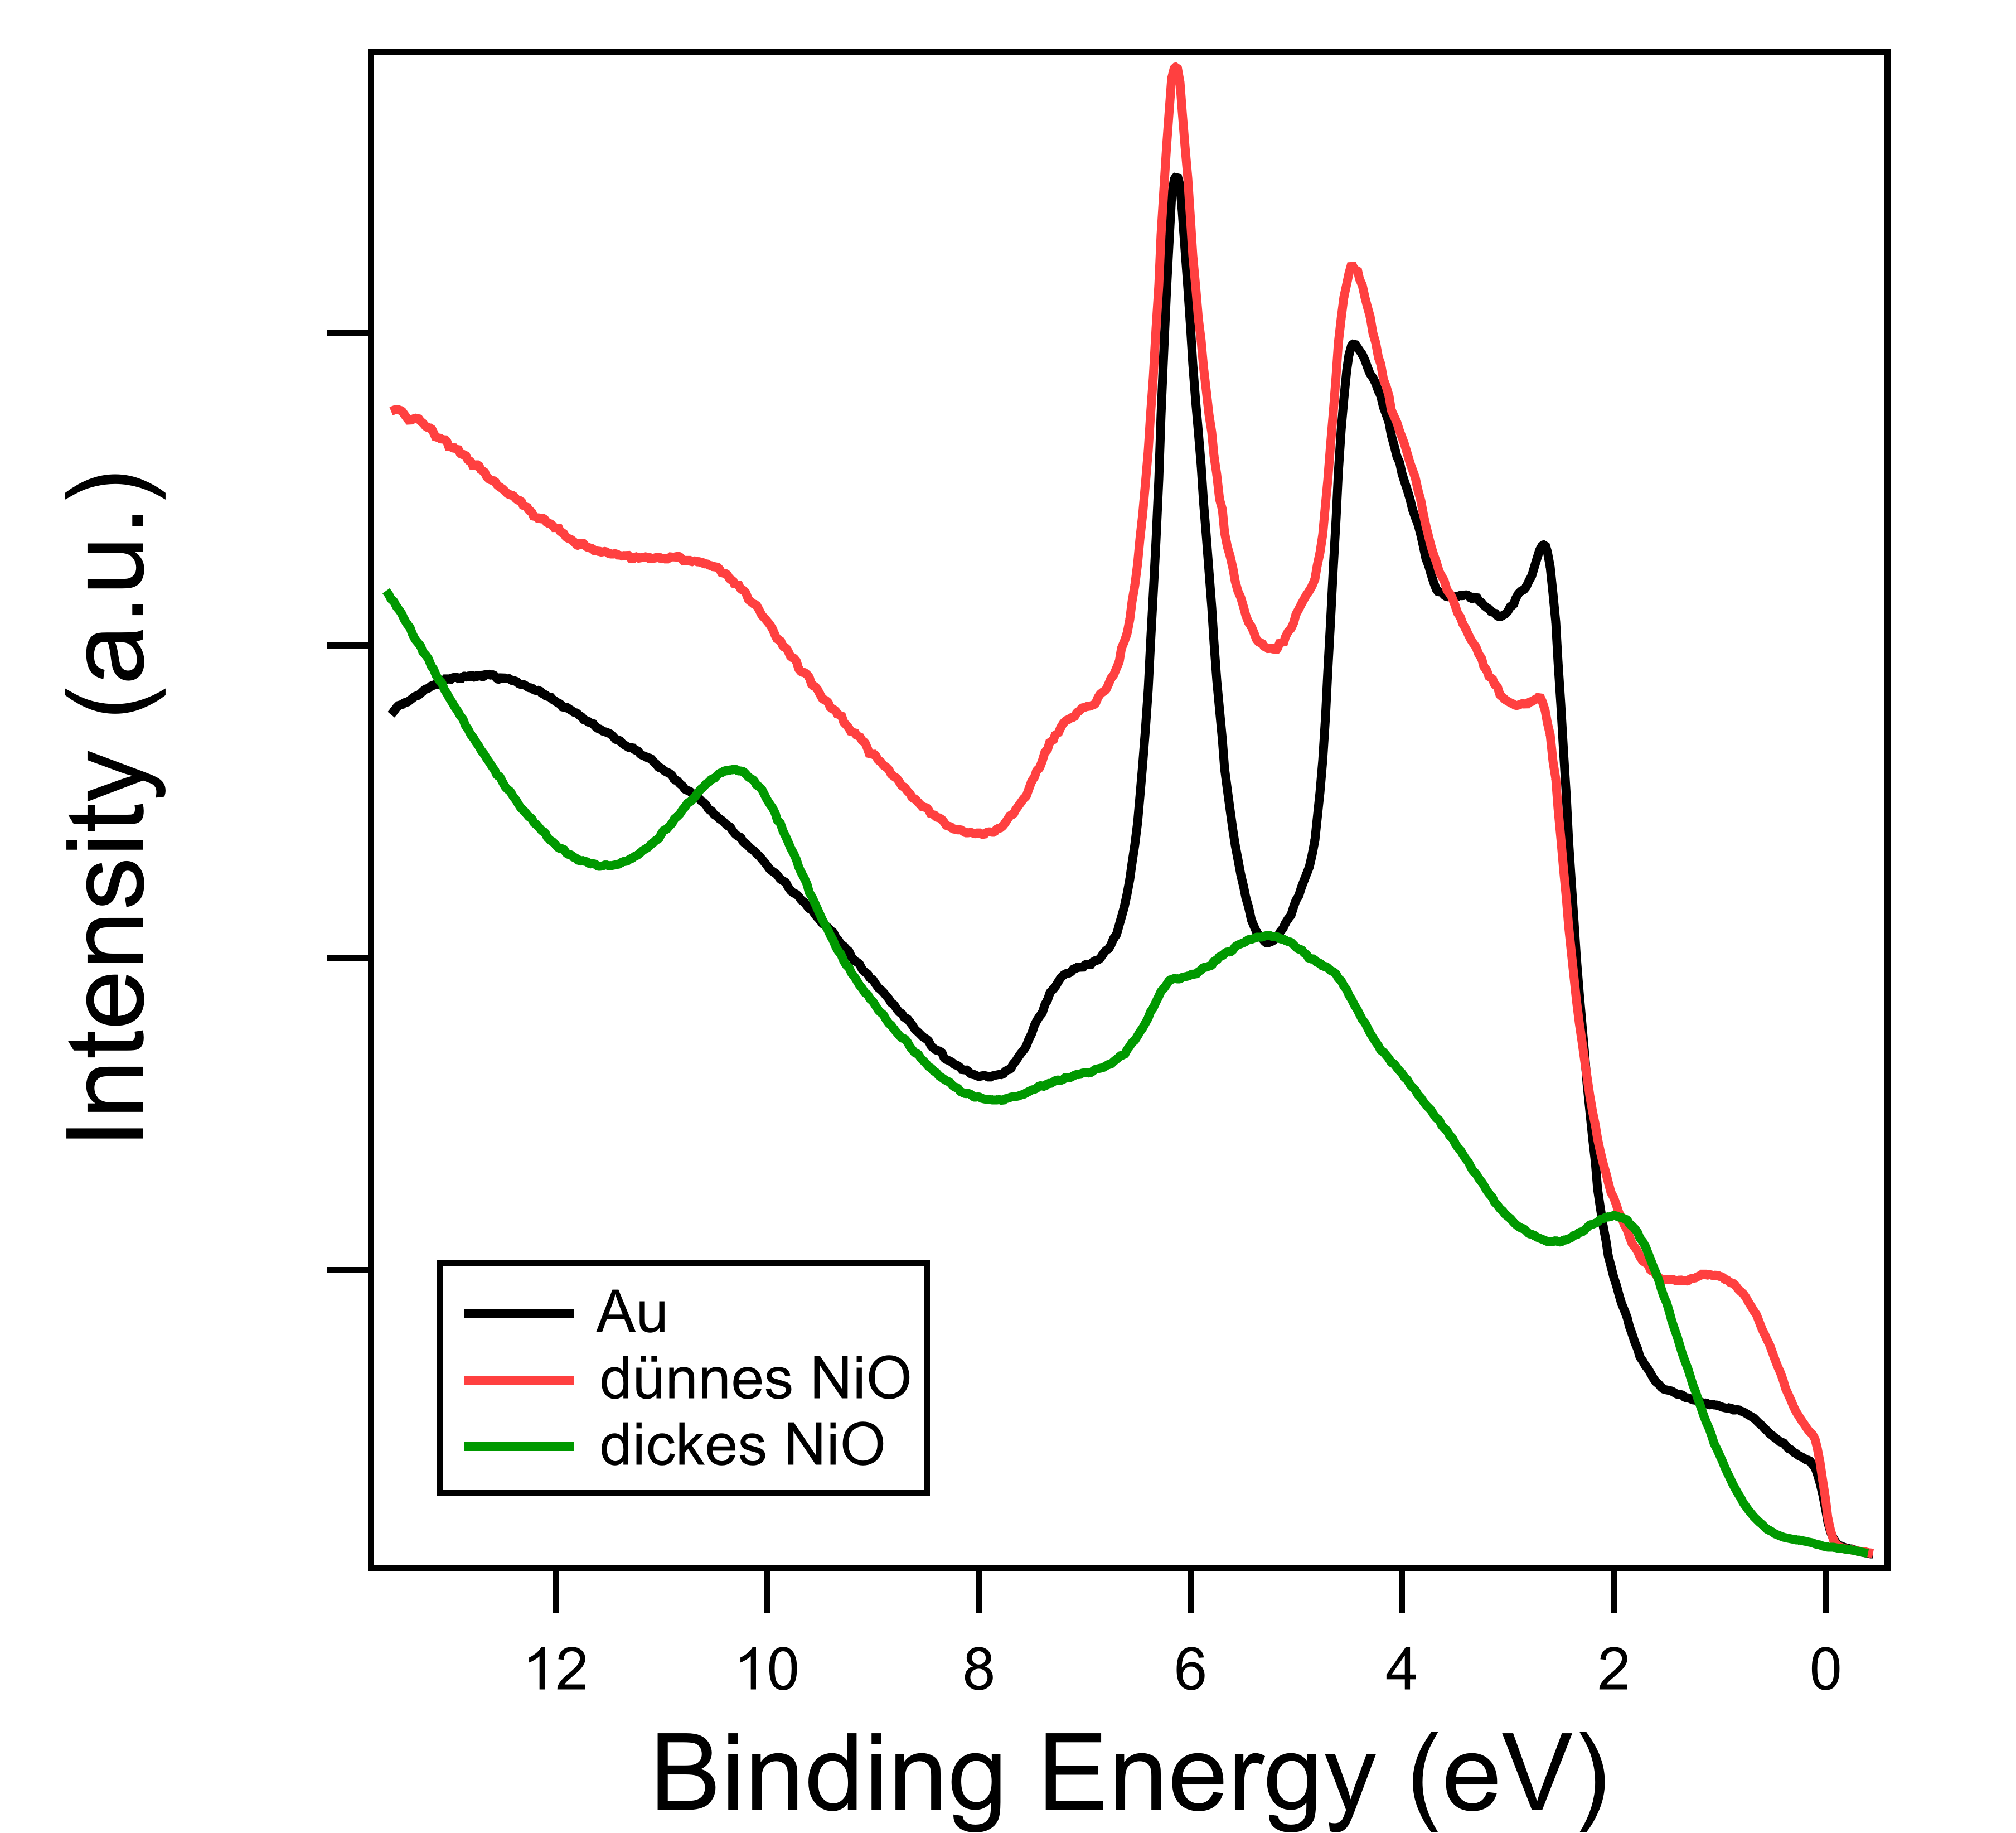
\includegraphics[width=0.6\textwidth]{./content/pictures/NiO_Filmdicke}
            \caption{Die integrierten Spektren für zwei verschiedene Schichtdicken von \ce{NiO}. Als Referenz dient das integrierte Spektrum von Gold.}
            \label{fig:NiO_Filmdicke}
        \end{figure}
        % \end{wrapfigure}
        Die Elektronendichtekurven für die reinen Substrate sind gemeinsam mit den der zusätzlich aufgebrachten Molekülen in den Abbildungen~\ref{fig:NiO+5A} und~\ref{fig:FeO+5A} dargestellt.
        Es lassen sich bei den in den Spektren erkennbare zusätzliche Merkmale erkennen die somit den Molekülen zugeordnet werden können.
        An diesen Punkten werden einzelne Bilder mit einer erhöhten Statistik aufgenommen.
        %   \begin{figure}
        %     \centering
        %     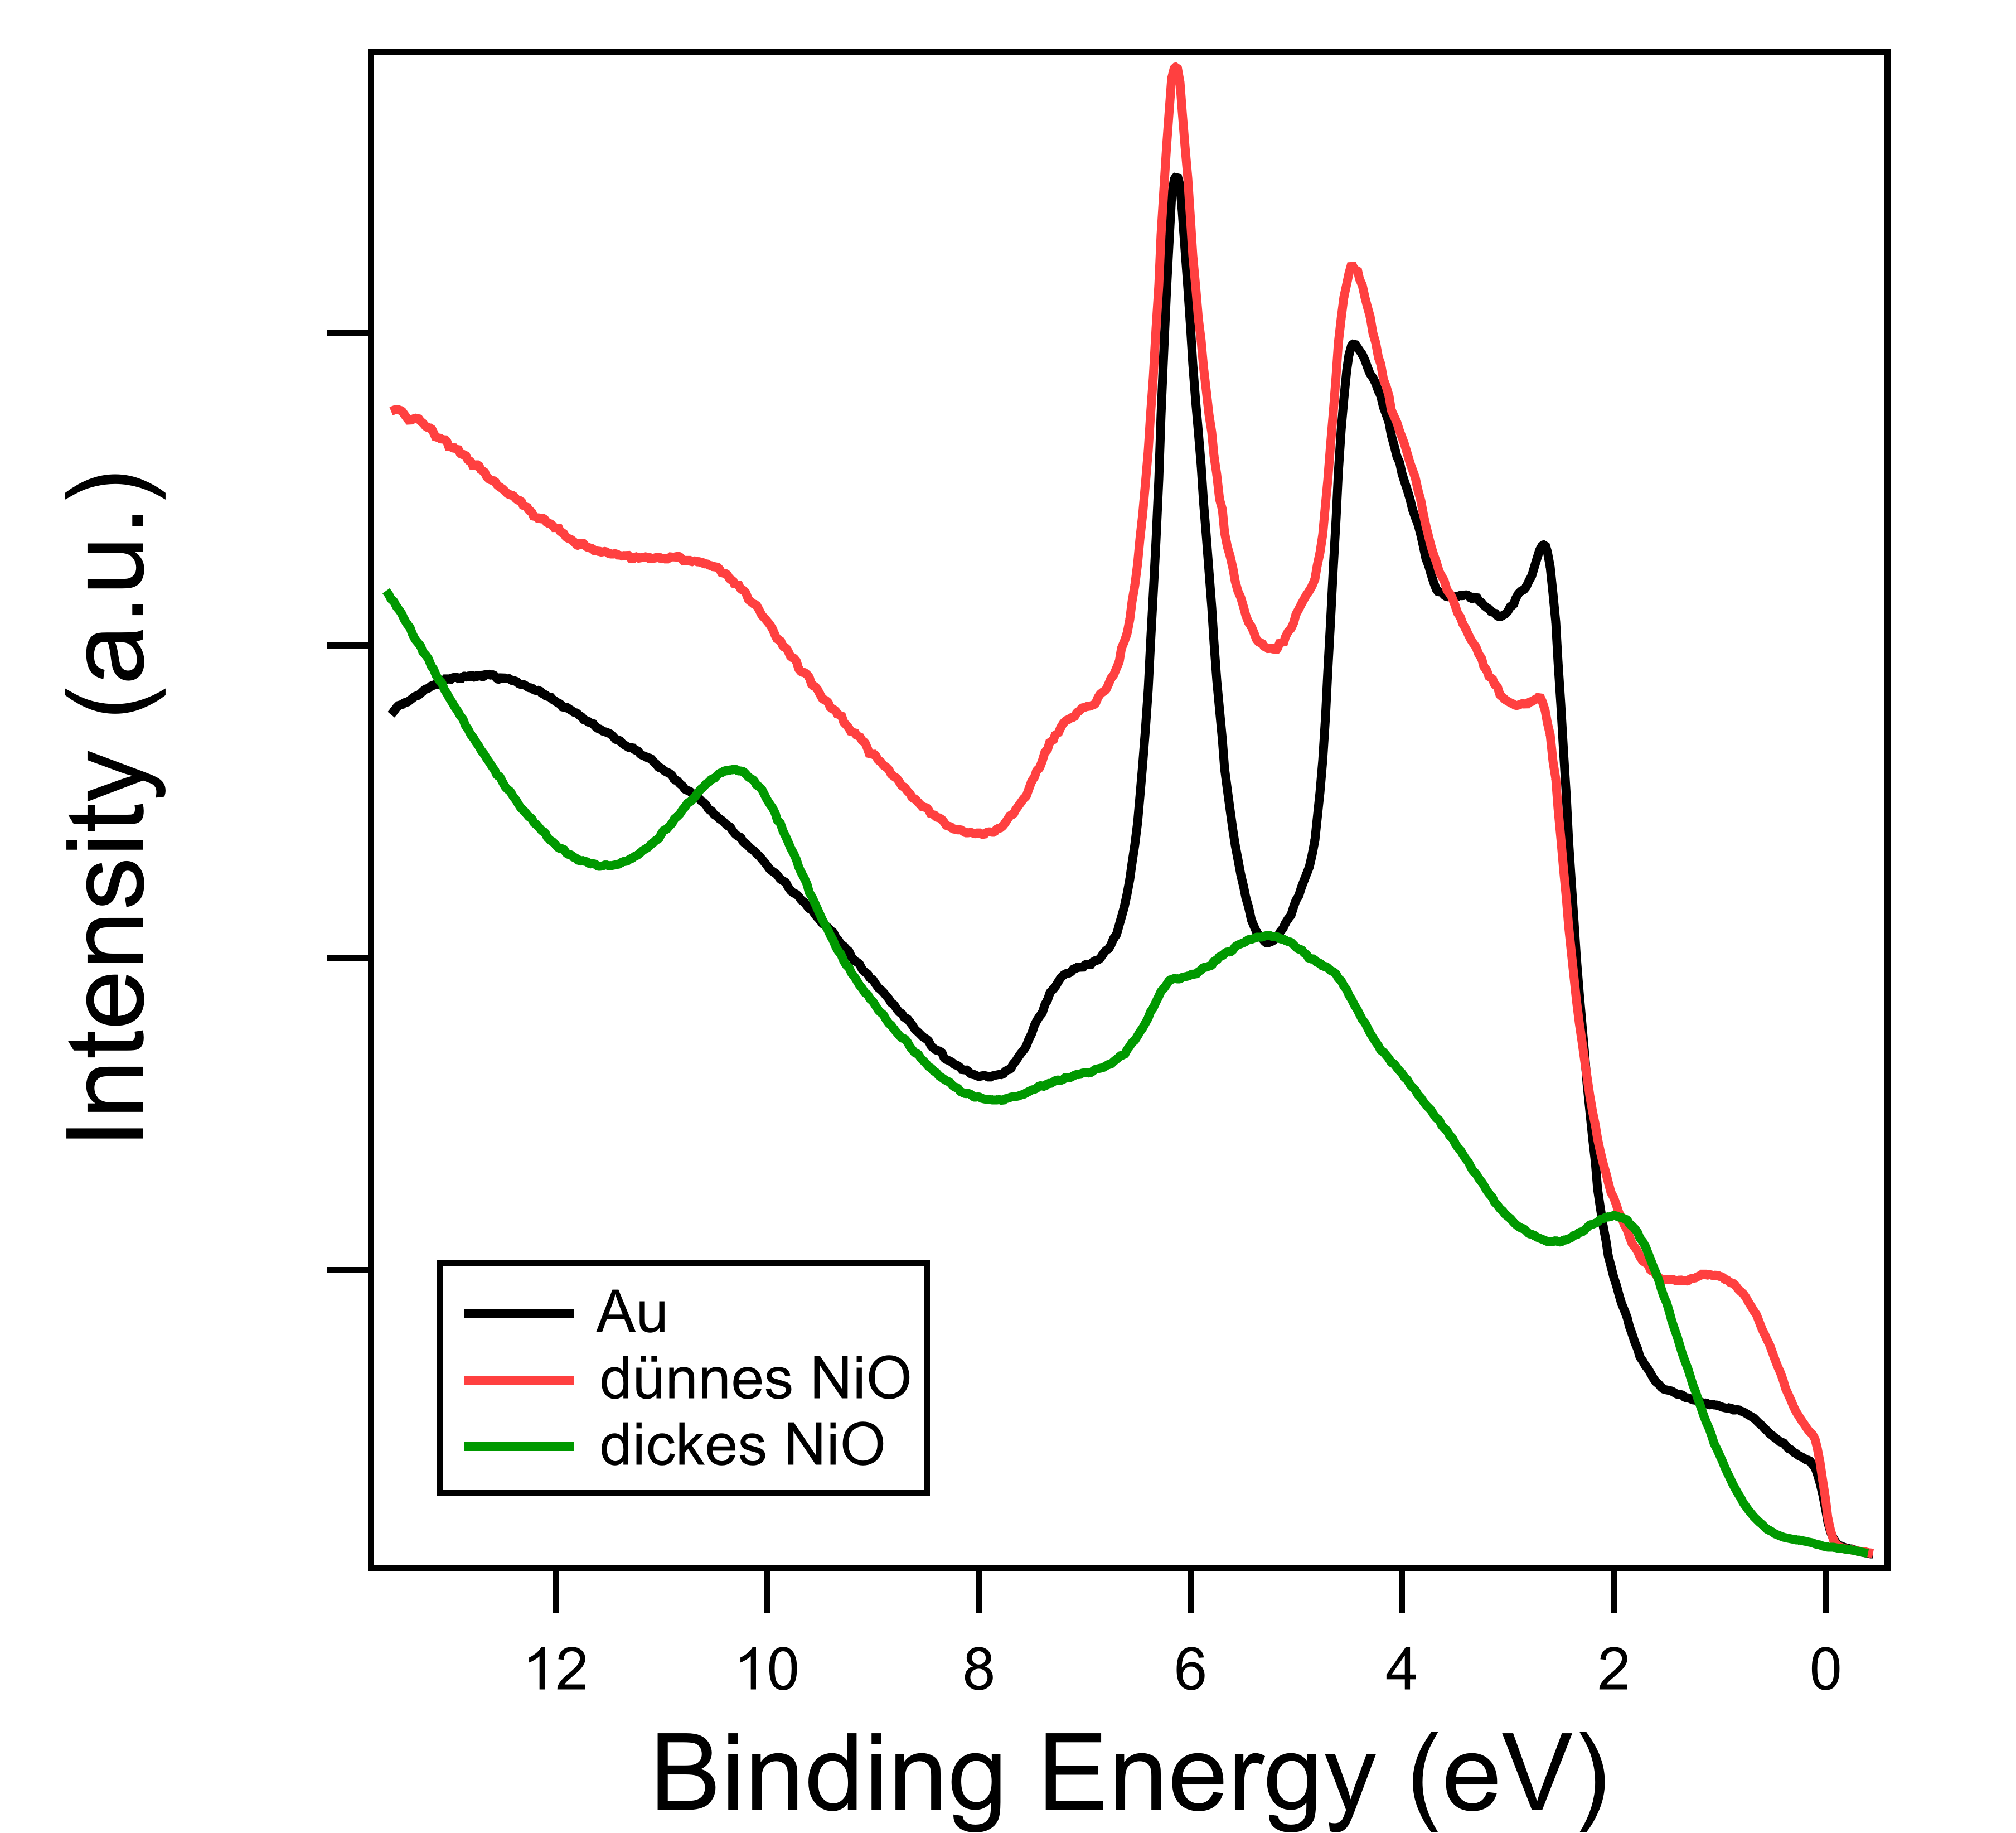
\includegraphics[width=0.7\textwidth]{./content/pictures/NiO_Filmdicke.png}
        %     \caption{Das Valenzbandspektrum von Nickeloxid im vergleich zu Messungen aus der Lieteratur.}
        %     \label{fig:NiO_Filmdicke}
        % \end{figure}
        Wird die gesamte Länge des Spektrums betrachtet, also der Energieunterschied zwischen Fermikante und Ende des Sekundärelektronen, so lässt sich die Austrittsarbeit der Probe bestimmen.
        So lässt sich erkennen, dass sich die Austrittsarbeit vom Gold zu dickeren Filmen Nickeloxid zu kleineren Werten verschiebt.
        Für Gold lässt sich die Austrittsarbeit auf \SI{5.46}{\electronvolt} ermitteln, was in der selben Ornung wie Literaturwerte liegt~\cite{Hüfner}.
        Vom dünnen Nickeloxidfilm zum dickeren Nickeloxidfilm wechselt sie von \SI{4.25}{\electronvolt} zu \SI{3.90}{\electronvolt}.
        Die Austrittsarbeit des dicken Nickeloxidfilms passt \textbf{Quelle und Wert}.
        Für das Eisenoxid ergibt sich eine Austrittsarbeit von \textbf{Wert sowie Literatur}.

        \begin{figure}
            \centering
            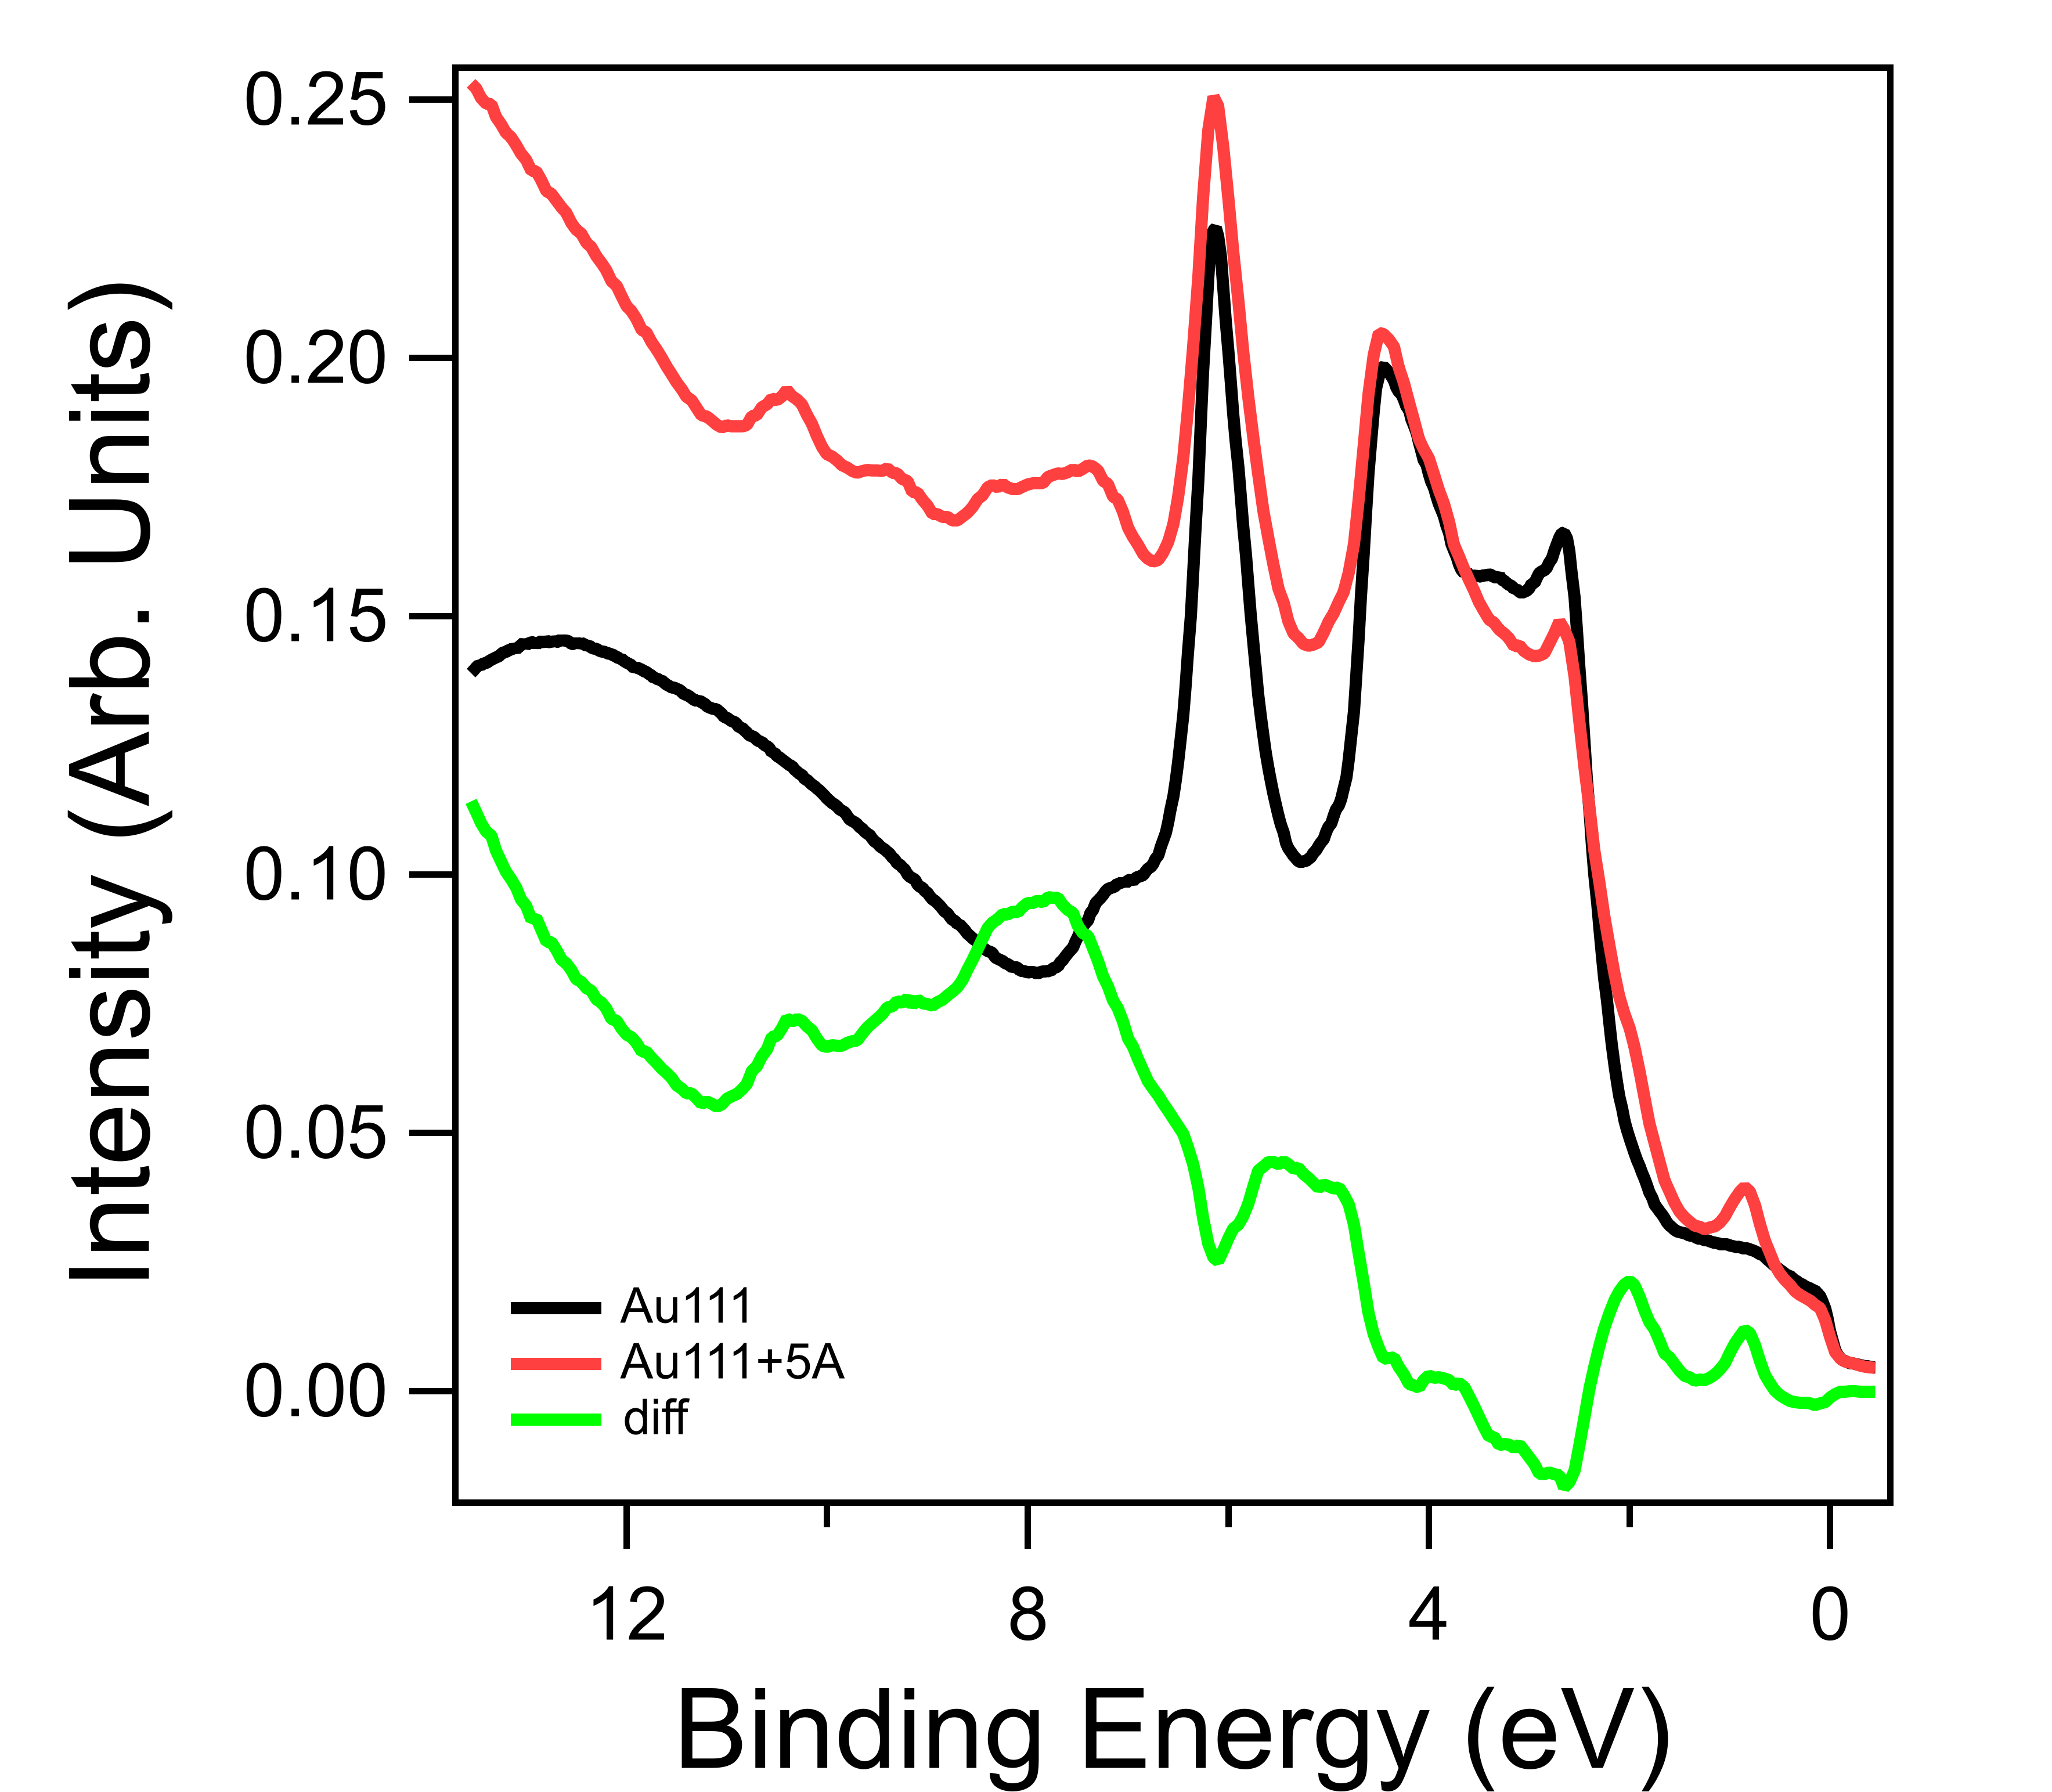
\includegraphics[width=0.6\textwidth]{./content/pictures/EDC_Au_5A.png}
            \caption{Die integrierten Spektren für reines Gold, Gold mit einer Monolage Pentacene und deren Differenz.}
            \label{fig:Au+5A}
        \end{figure}

        \begin{figure}
            \centering
            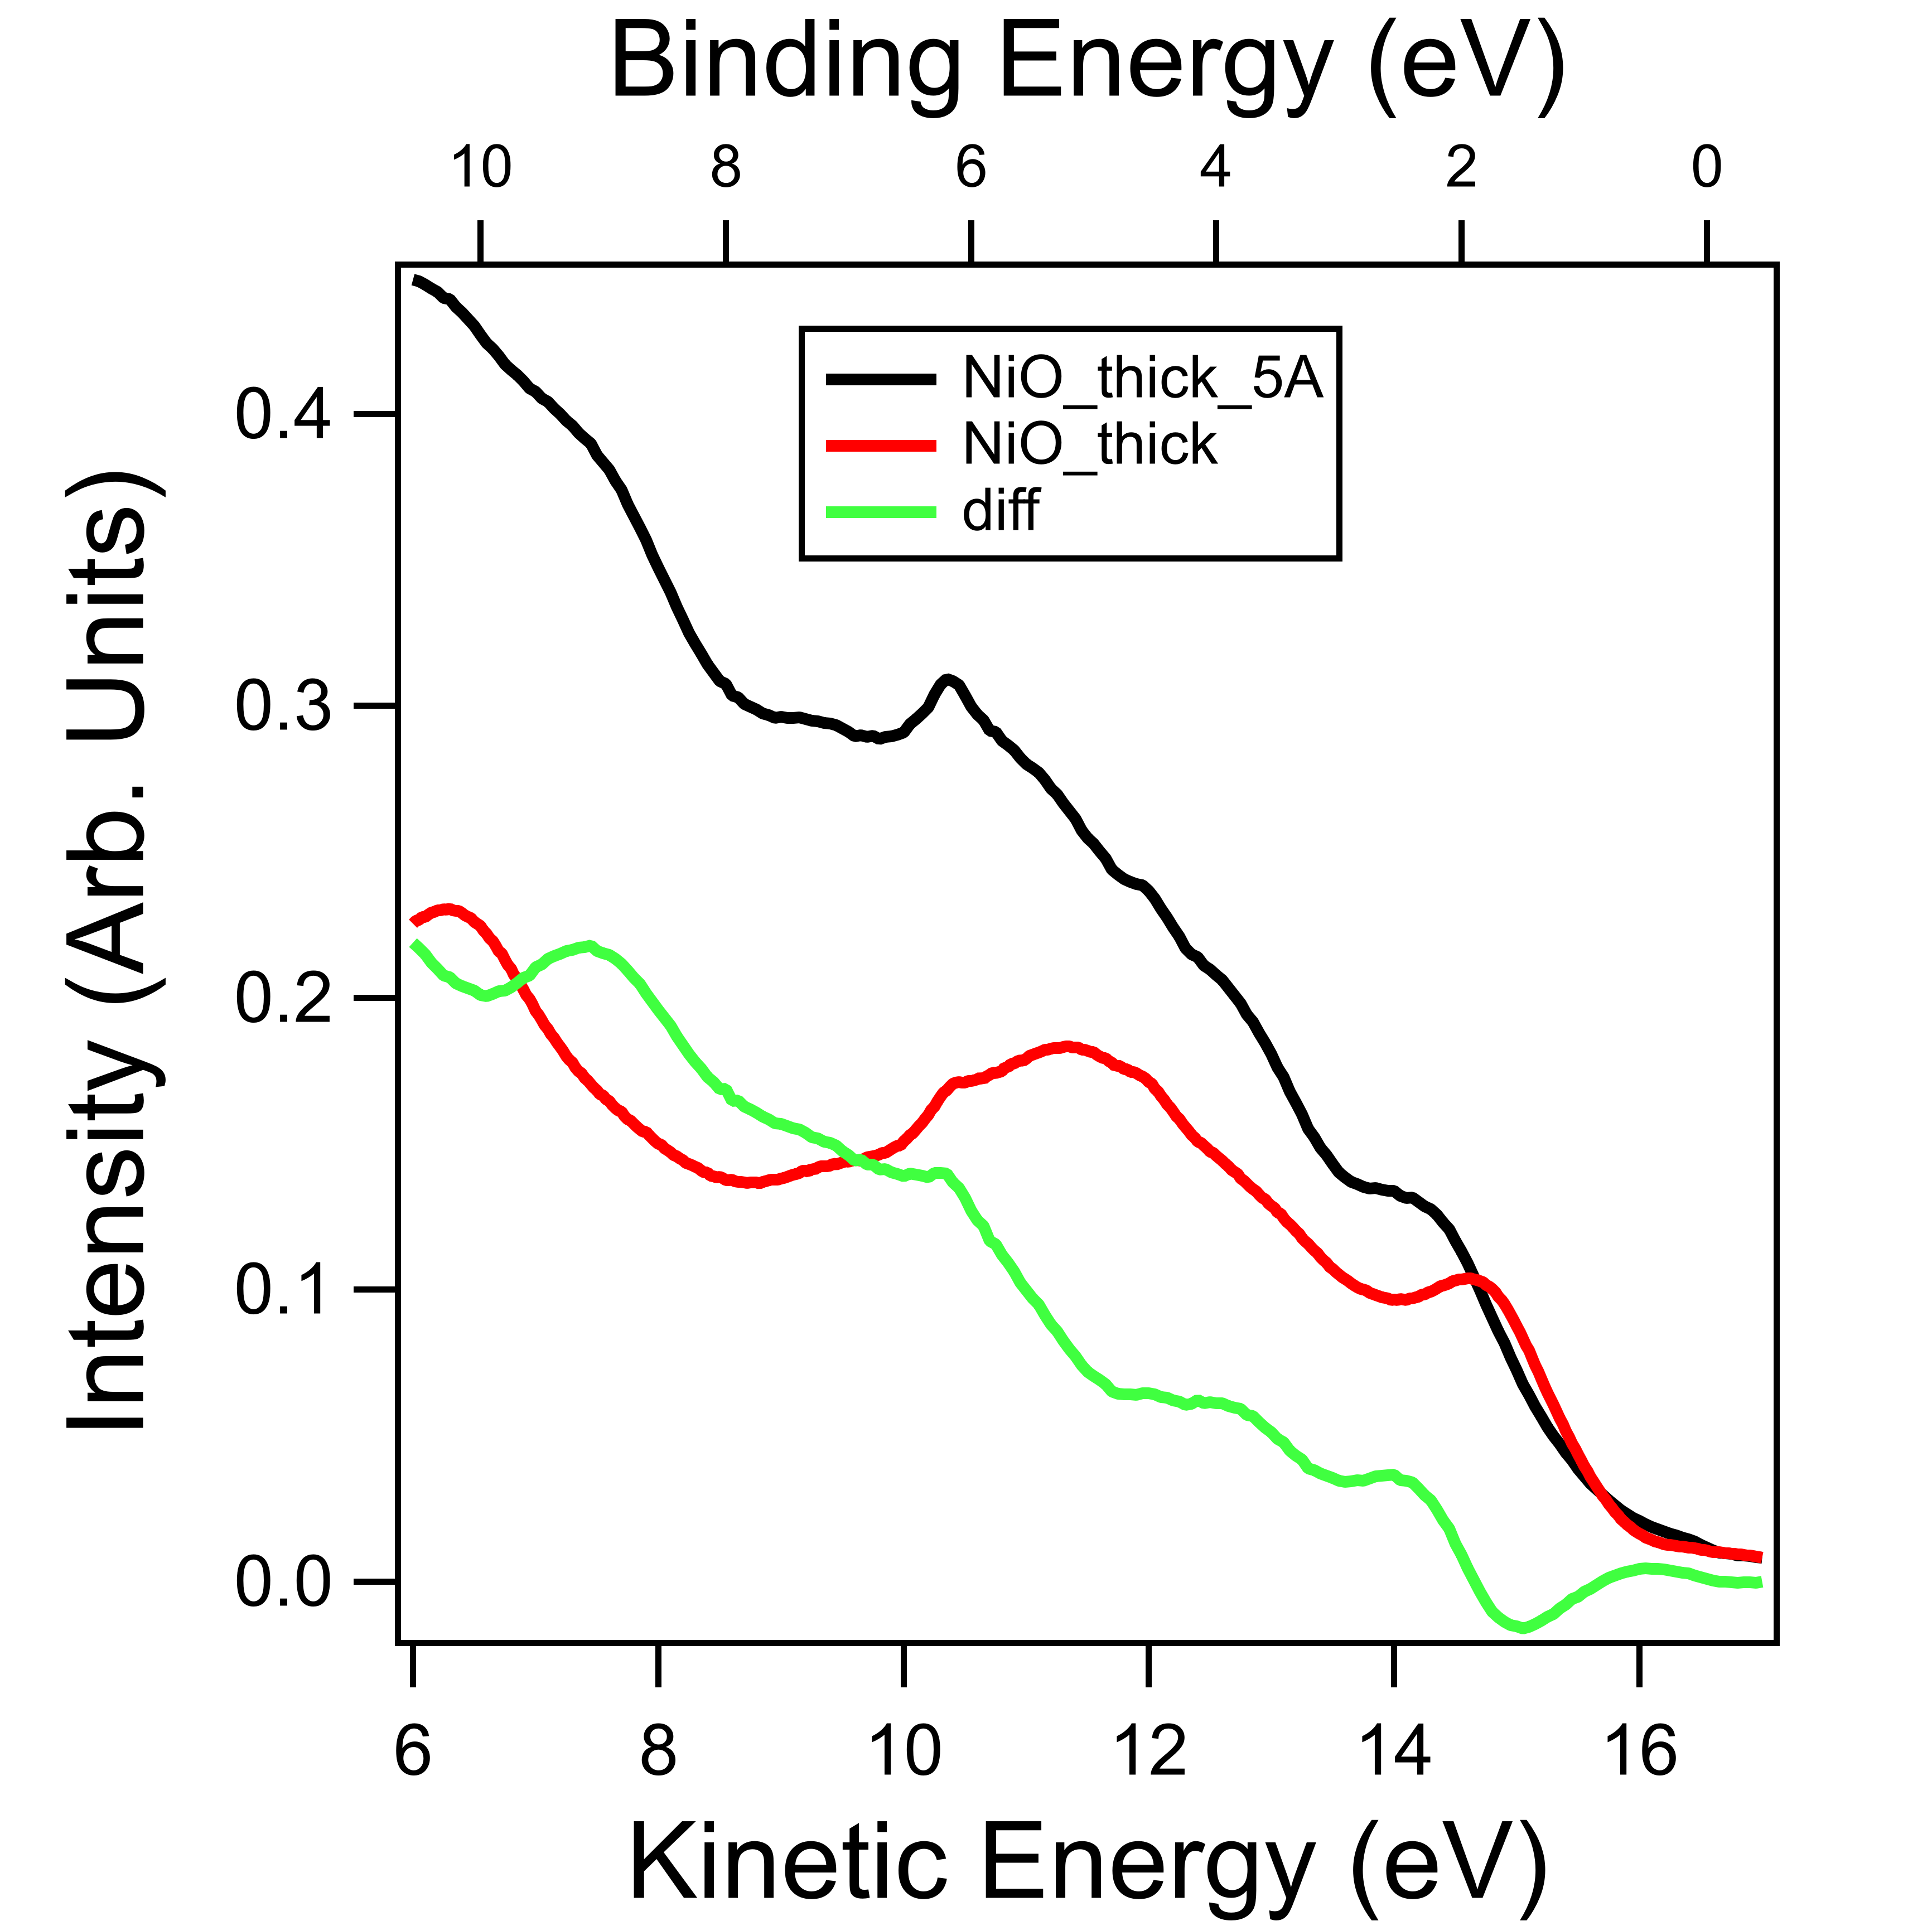
\includegraphics[width=0.6\textwidth]{./content/pictures/NiO_thick_5A.png}
            \caption{Die integrierten Spektren für einen dicken Nickeloxidfilm, mit zusaätzlich einer Monolage Pentacene und deren Differenz.}
            \label{fig:NiO+5A}
        \end{figure}

        \begin{itemize}
            \item Sieht Features später Zuordnung
            \item Ändert sich was
            \item Verbreiterung Lebenszeit, Linienbreite Photonenquelle, Thermisch, Analysator
        \end{itemize}

    \section{Bandstruktur}
        \begin{figure}
            \centering
            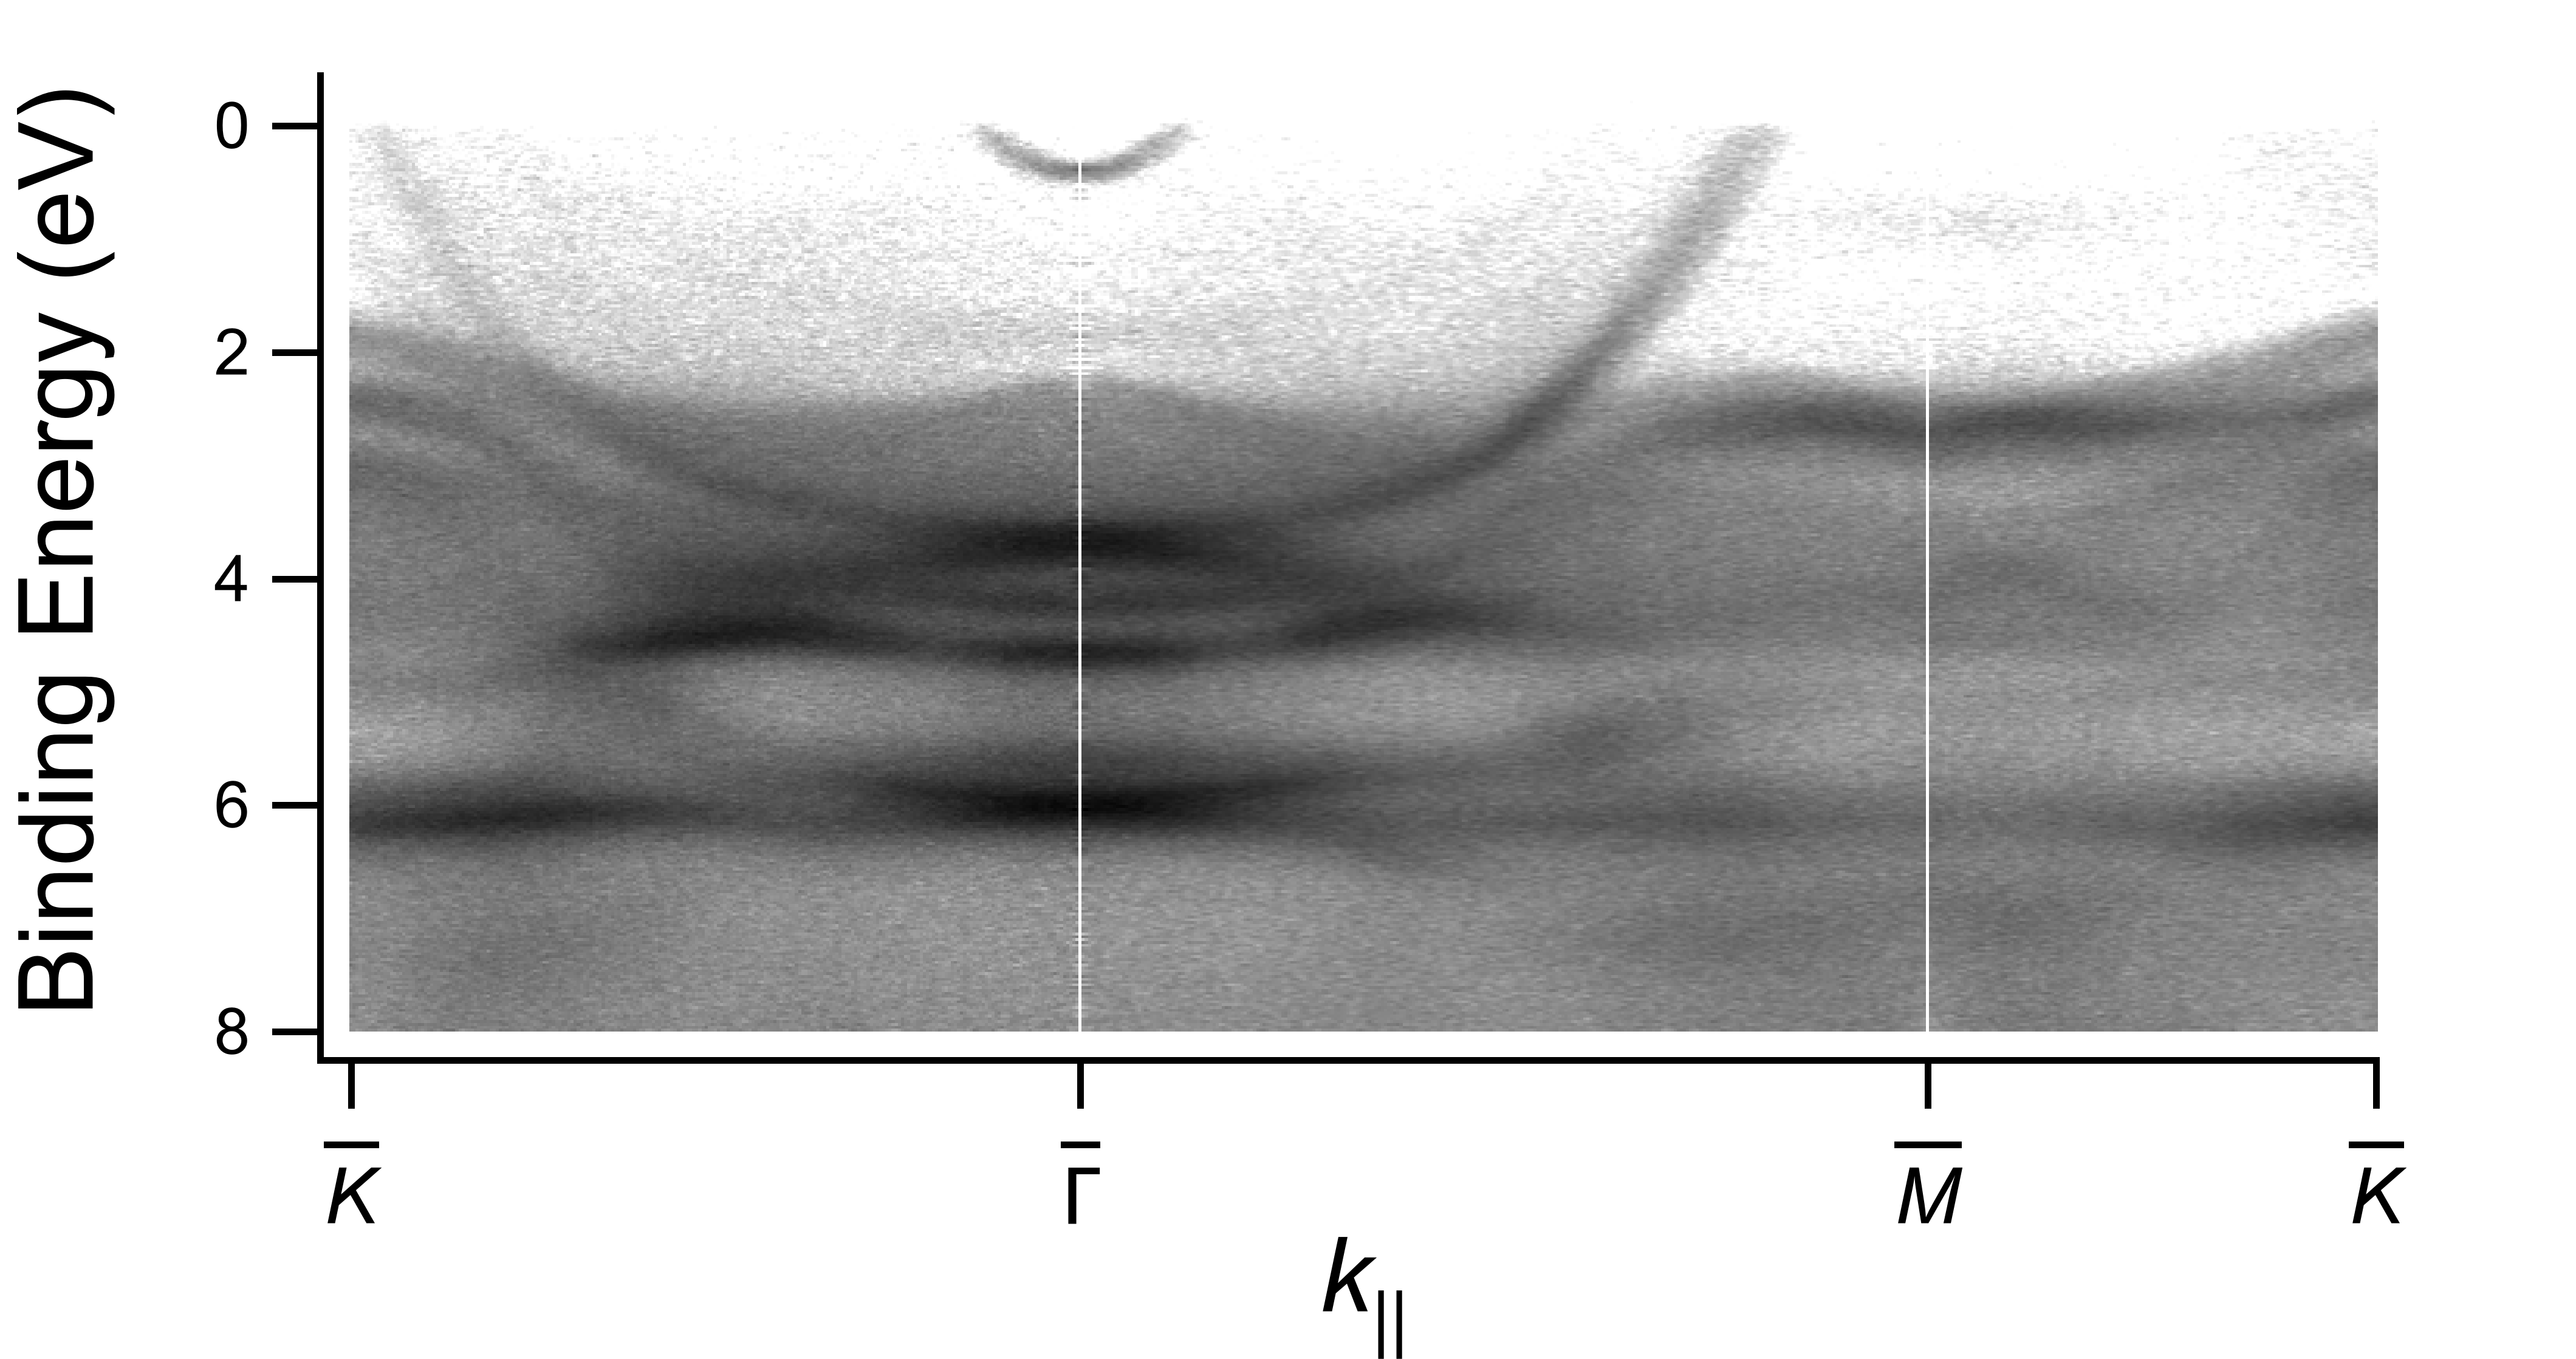
\includegraphics[width=0.7\textwidth]{./content/pictures/Bandstructure_Au111.png}
            \caption{Die gemessene Bandstruktur von Gold (111).}
            \label{fig:Bandstructure_Au}
        \end{figure}
        \begin{figure}
            \centering
            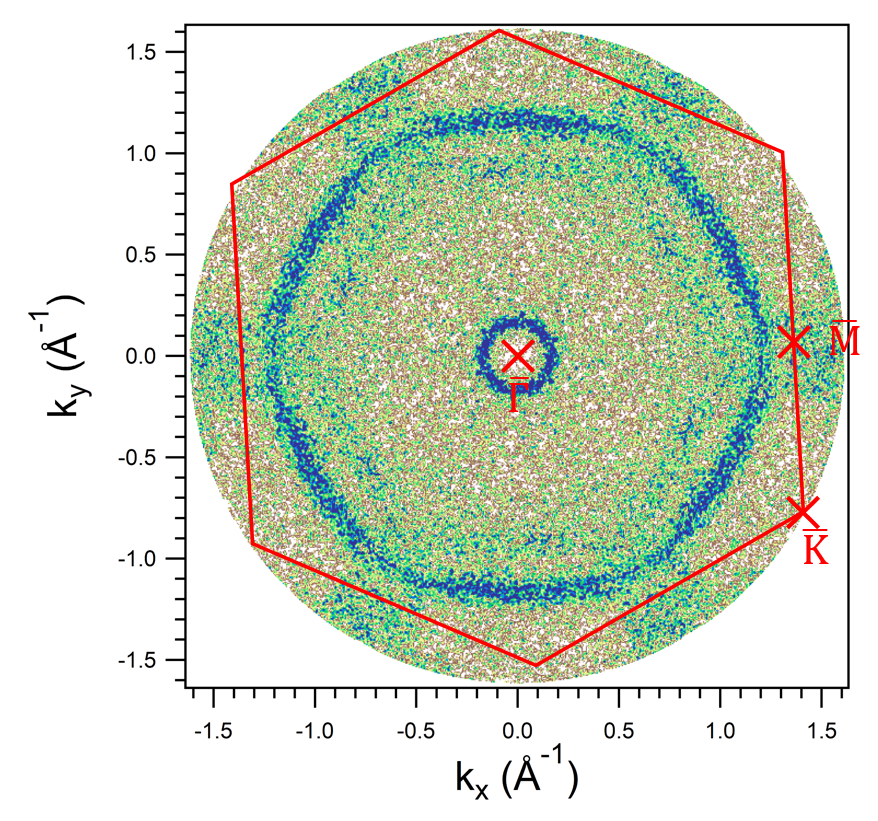
\includegraphics[width=0.7\textwidth]{./content/pictures/BZ}
            \caption{Die gemessene Winkelverteilung von Gold (111) an der Fermifläche.
            Eingezeichnet in rot ist die erste Brillouinzone und drei Hochsymmetriepunkte, entlang deren Richtung der Stack für die Bandstruktur geschnitten wird.}
            \label{fig:BZ}
        \end{figure}
        In \autoref{fig:Bandstructure_Au} lässt sich die Bandstruktur erkennen, welche aus dem Stack entlang einiger Hochsymmetrierichtungen extrahiert wurde.
        Der Schnitt ist in \autoref{fig:BZ} veranschaulicht.


        \begin{itemize}
            \item Bandstruktur von Gold
            \item Bandstruktur NiO? Spin?
            \item Bandstruktur mit Molekülen - Oberflächenzustände? Extra Features
        \end{itemize}

    \section{Molekülorbitaltomographie}
        In den Bildern von Pentacene auf Nickel- und Eisenoxid lassen sich leider keine Molekülorbitale zuordnen.
        Die Ursache ist, dass wie bereits im \autoref{sec:Praep} anhand der LEED Bilder festgestellt wurde, die Moleküle sich nicht regelmäßig auf der Oberfläche anordnen.
        Ferner überlappen dann die einzelnen Merkmale im Impulsraum, sodass ein ausgewaschenes Bild entsteht.

        Wenn hingegen die Moleküle auf dem reinen Goldkristall aufgebracht werden er gibt sich eine periodische Struktur.
        Dies lässt sich anhand von LEED Bildern erkennen, ebenso in der Möglichkeit die Bilder im Impulsraum den theoretisch ermittelten Molekülorbitalen zuzuordnen, wie es in der \autoref{fig:MOT} geschehen ist.
        Hierzu wurden auf die berechneten Bilder die selben symmetrisierungs Schritte angewendet wie auf die gemessenen.

        Der größte Unterschied zwischen dem Gold und den Oxiden ist deren isolierenden Eigenschaften, es lässt sich also vermuten, dass für die Ornung Leitfähigkeit voraus gesetzt wird.
        Die theoretisch berechneten Maps wurden mit Hilfe des Python Programms \textit{kmap.py} erstellt~\cite{brandstetter_kmappy_2021}.

        \begin{itemize}
            \item Maps selbst die sich zuordnen lassen
            \item Aus den LP bestimmte zuordnung möglich?
        \end{itemize}

        \subsection{5A auf Au}
        \textbf{6 Bilder in einem Bild}
            \begin{figure}
                \centering
                \begin{subfigure}[t]{0.48\textwidth}
                    \centering
                    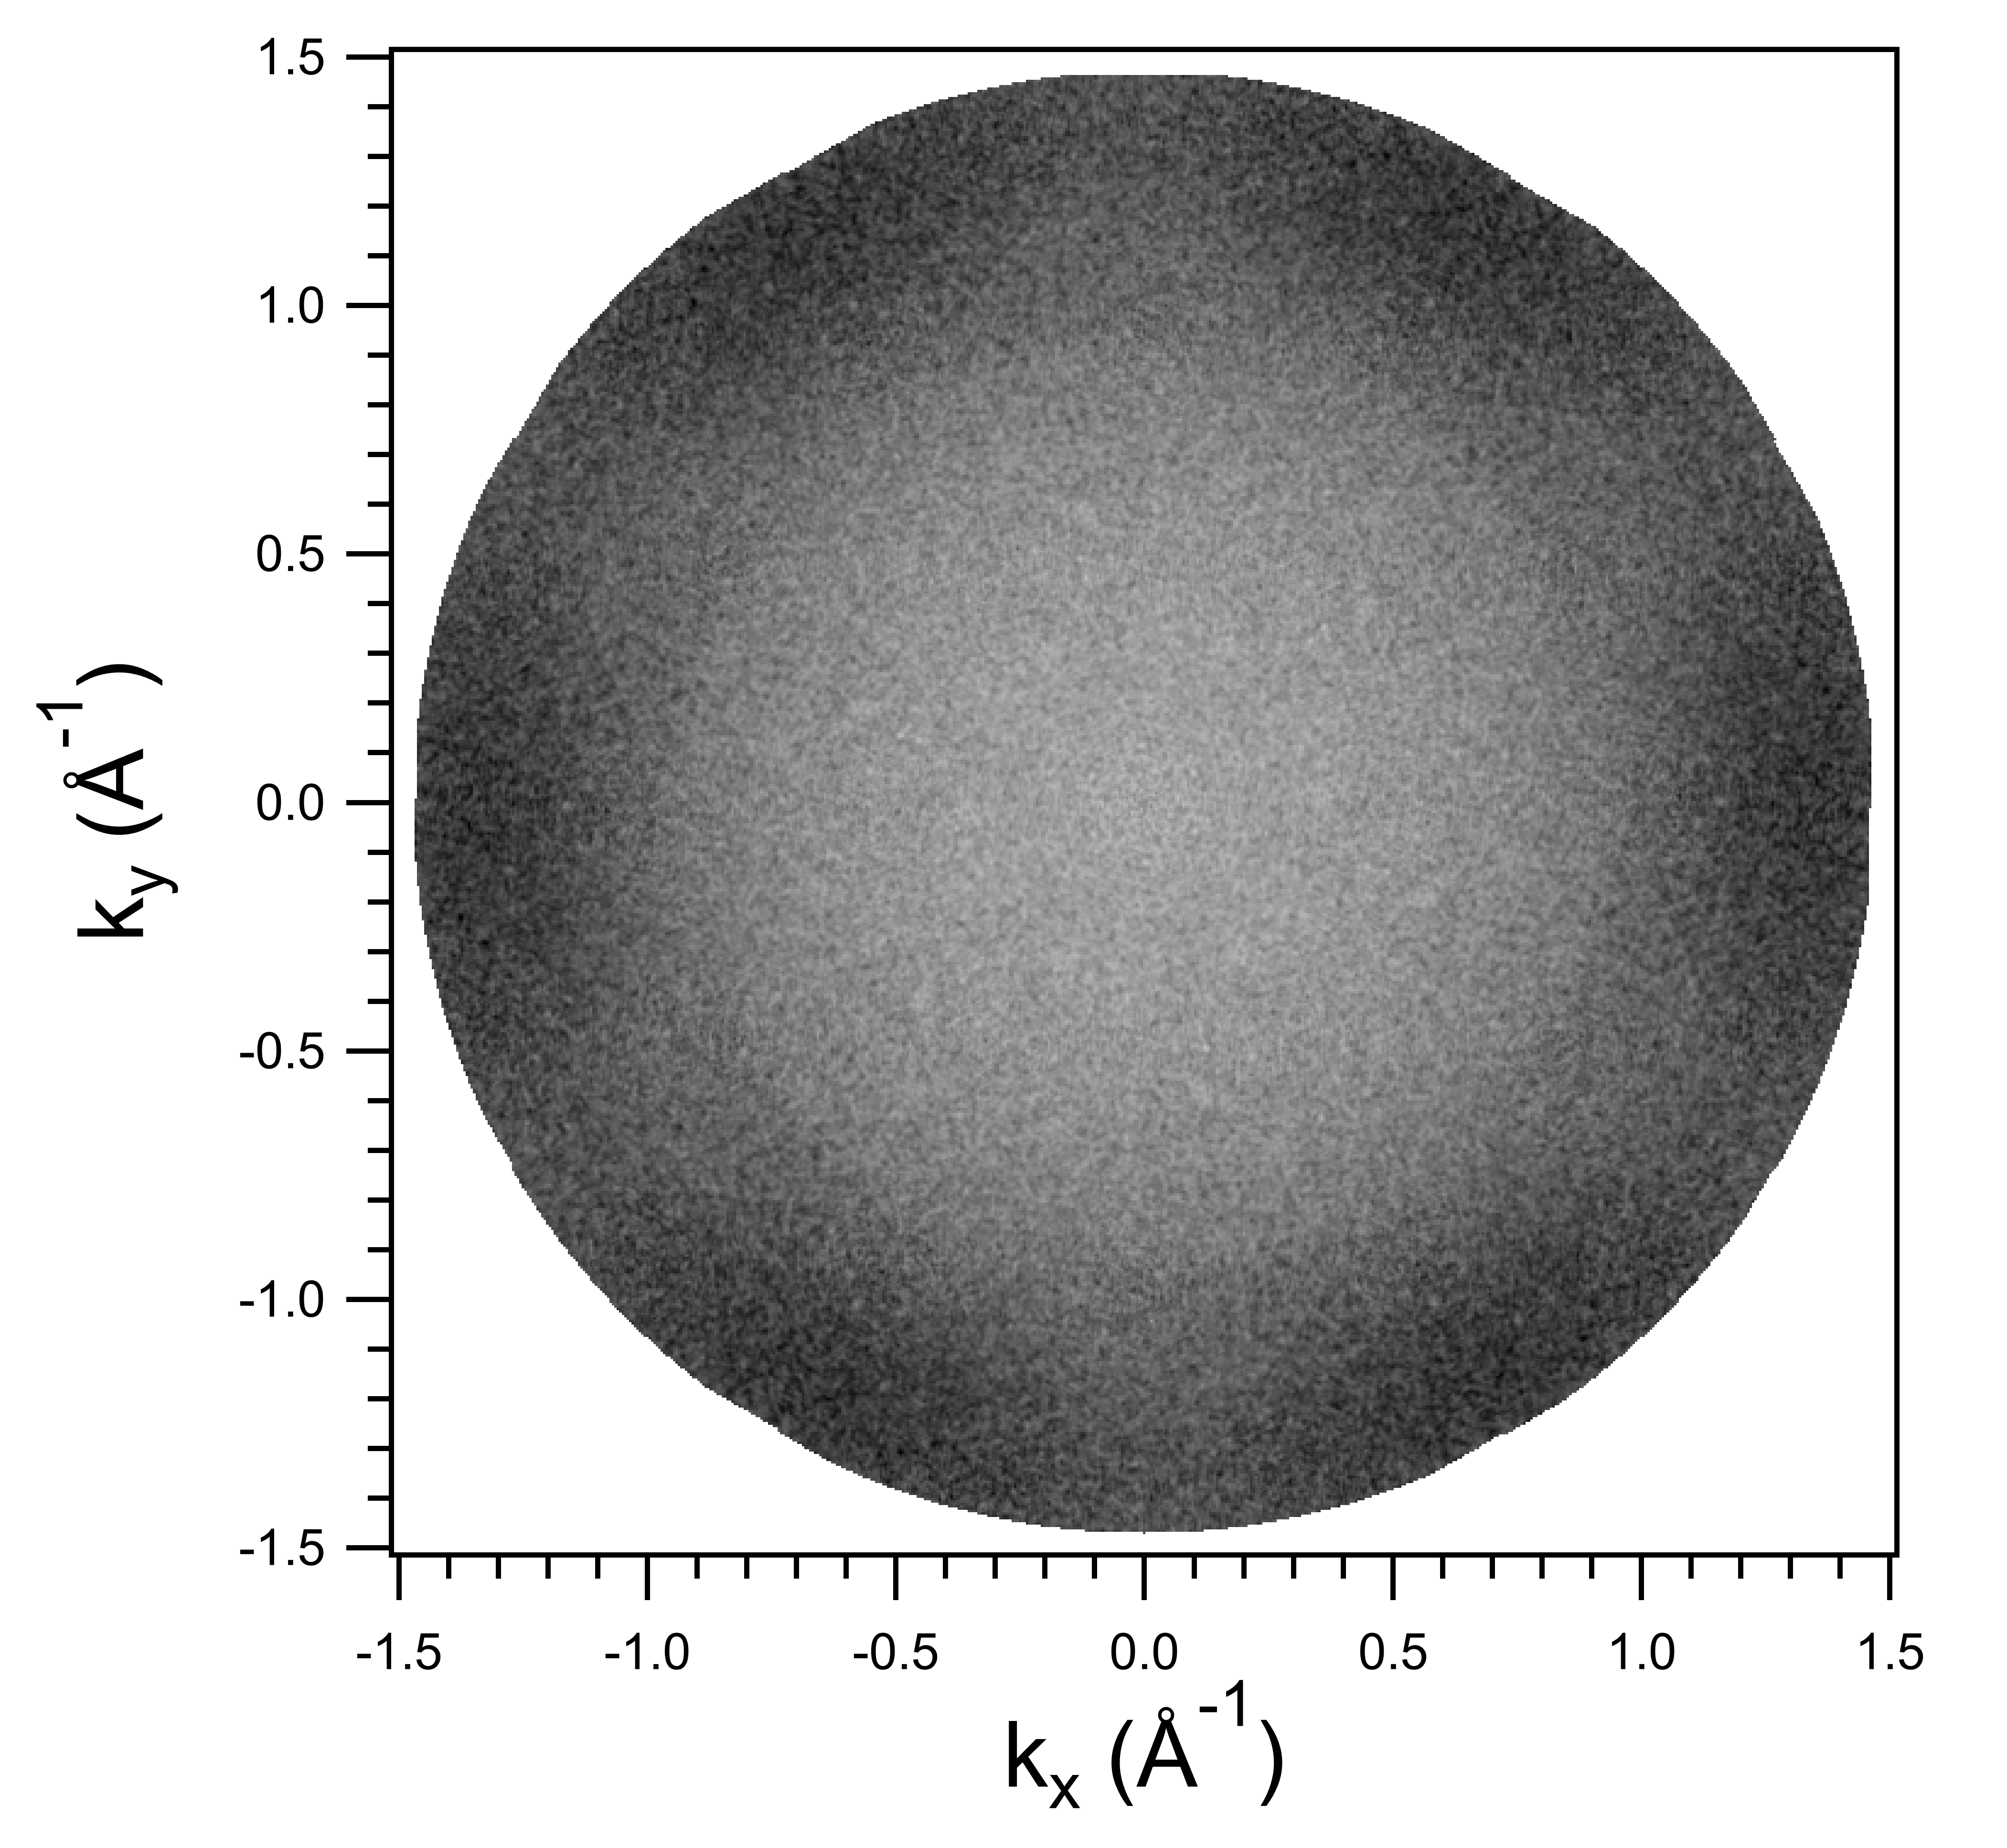
\includegraphics[height=5cm]{./content/pictures/Au+5A/IMAGE_2021_06_17_005_BE0_8}
                    \subcaption{Gemmesen, symmetrisiertes Bild bei einer Bindungsenergie von \SI{0.8}{\electronvolt}.}
                \end{subfigure}
                \begin{subfigure}[t]{0.48\textwidth}
                    \centering
                    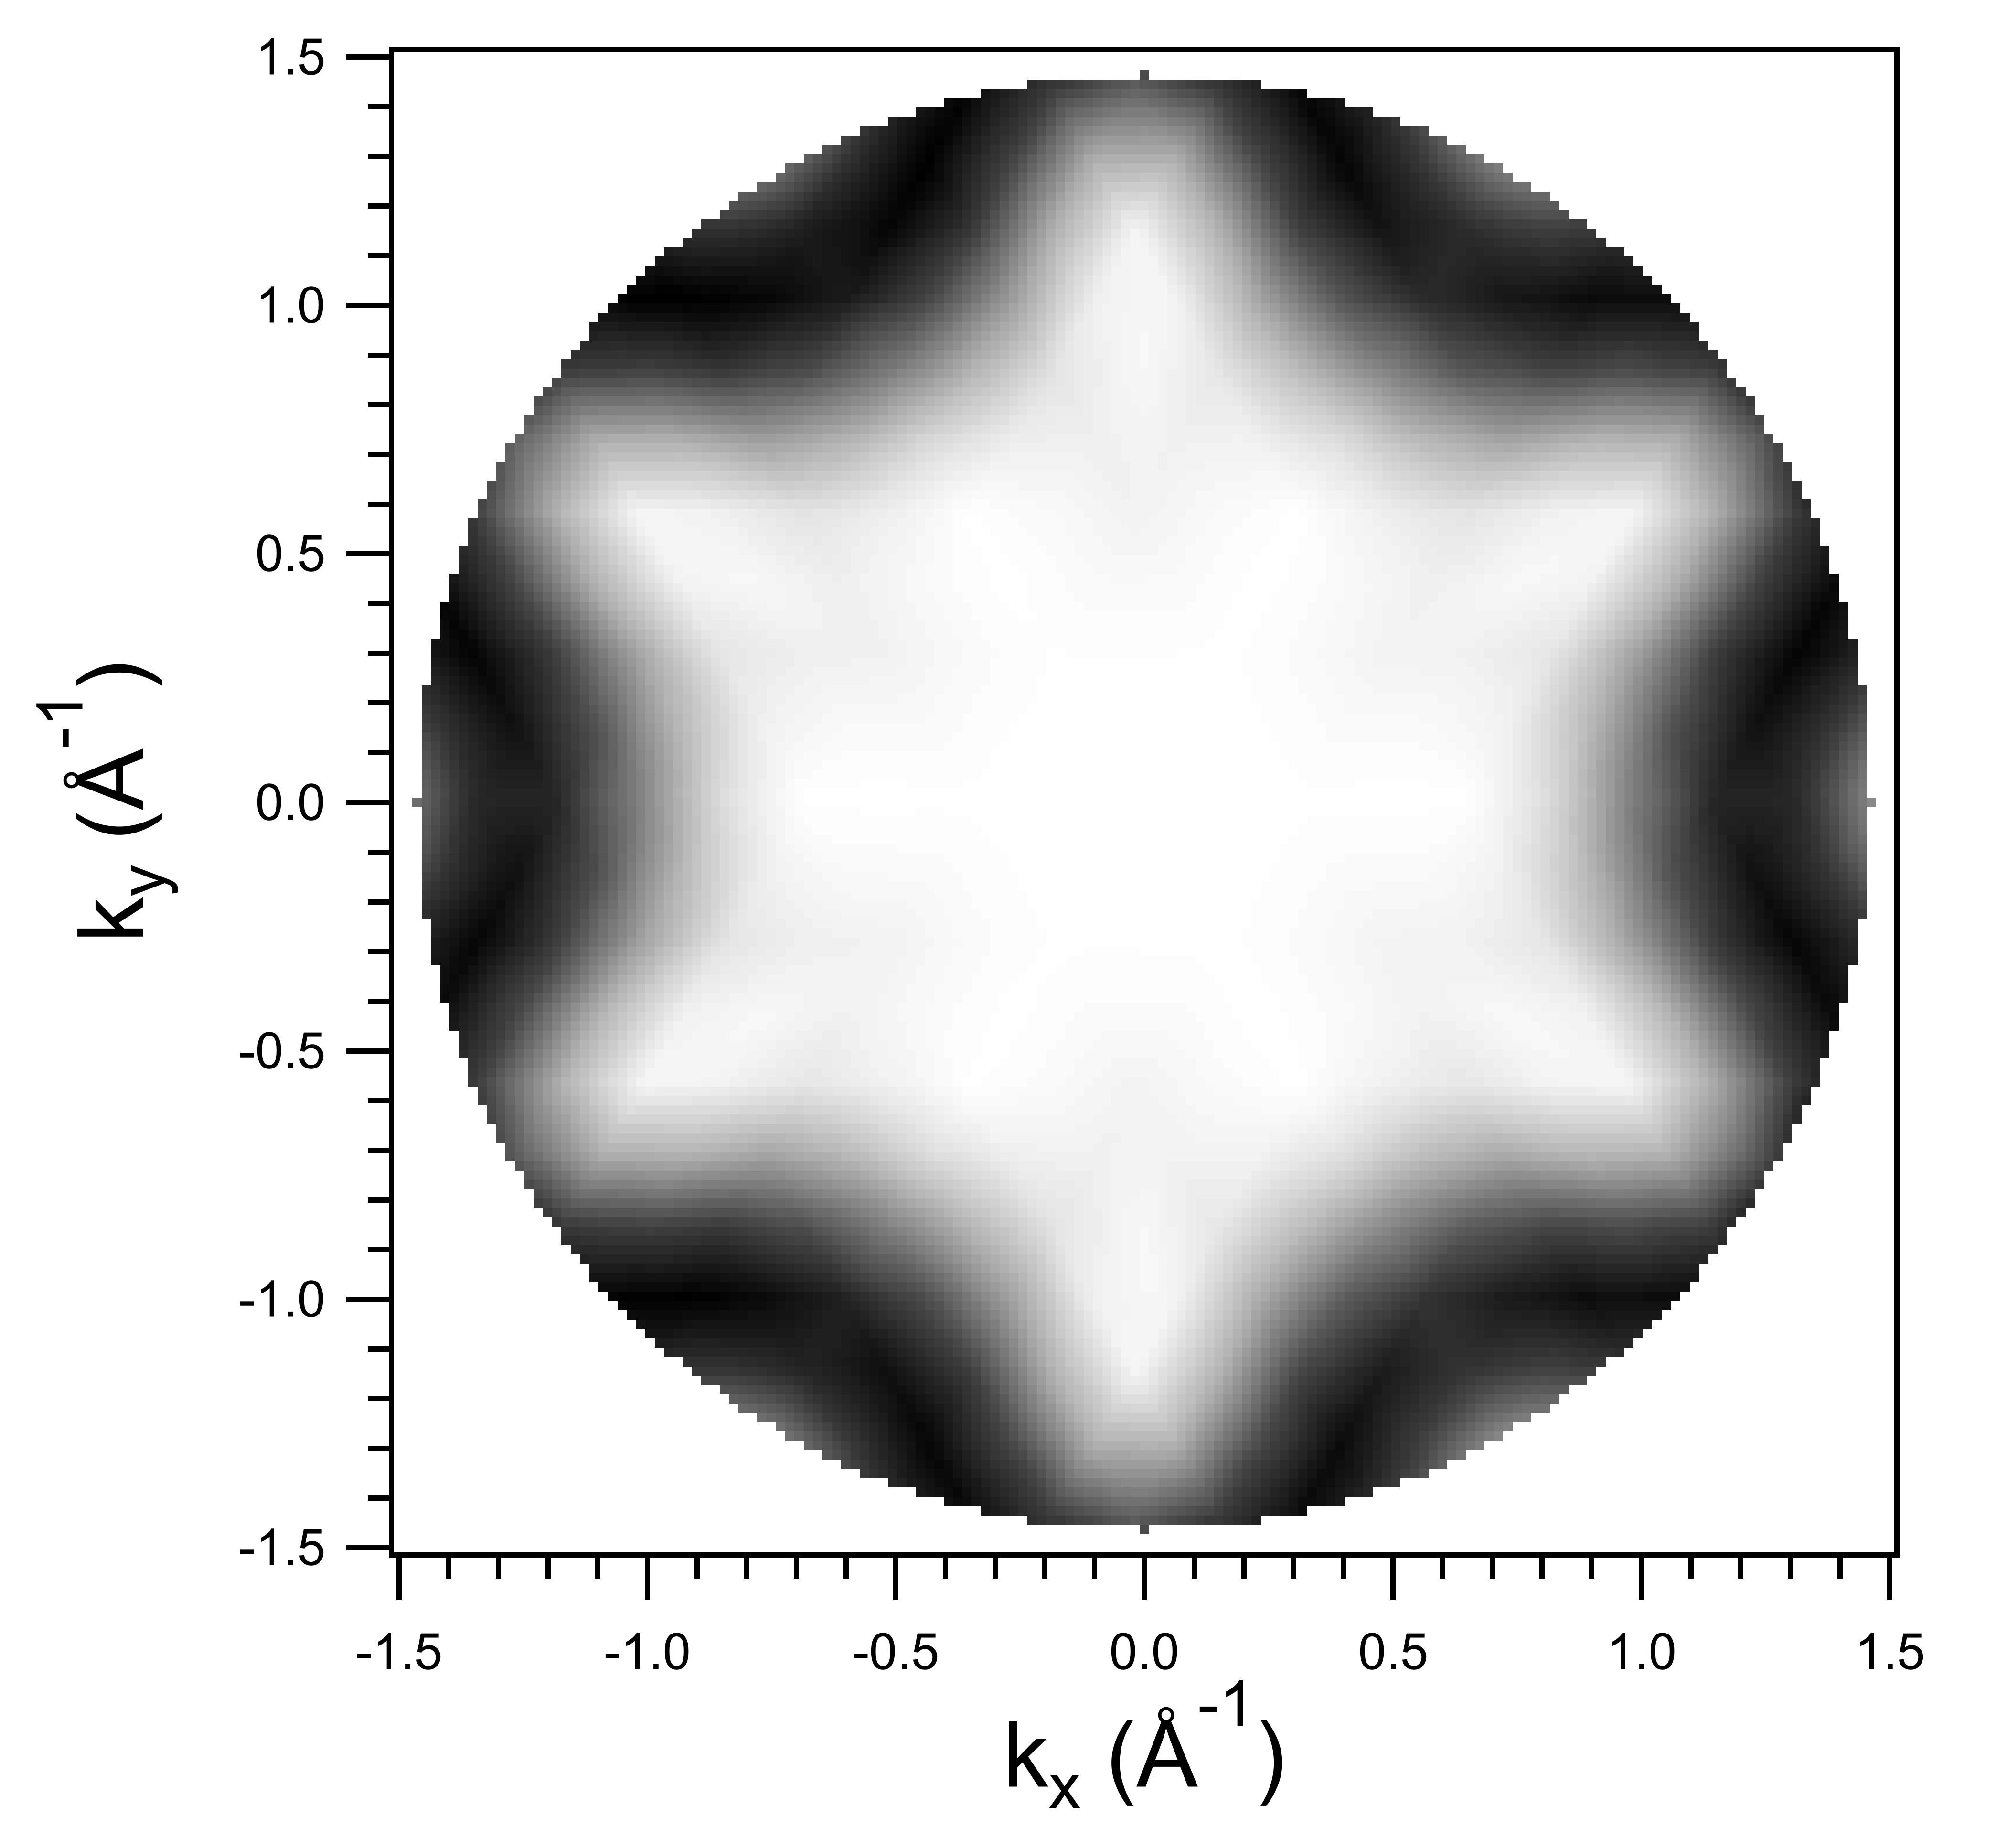
\includegraphics[height=5cm]{./content/pictures/Au+5A/HOMO1_all_CT}
                    \subcaption{Theorie Oribtale mit symmetrisierung 2mal um 120 Grad gedreht und zum Ursprungsbild addiert.}
                \end{subfigure}
                \caption{Zuordnung eines Bildes zu einem der Molekülorbitale.}
                \label{fig:MOT}
            \end{figure}
            % \begin{figure}
            %     \centering
            %     \begin{subfigure}{0.48\textwidth}
            %         \centering
            %         \includegraphics[height=5cm]{./content/pictures/Au+5A/IMAGE_2021_06_17_006_BE1_85.pdf}
            %         \subcaption{Gemmesen, symmetrisiertes Bild bei einer Bindungsenergie von \SI{1.85}{\electronvolt}.}
            %     \end{subfigure}
            %     \begin{subfigure}{0.48\textwidth}
            %         \centering
            %         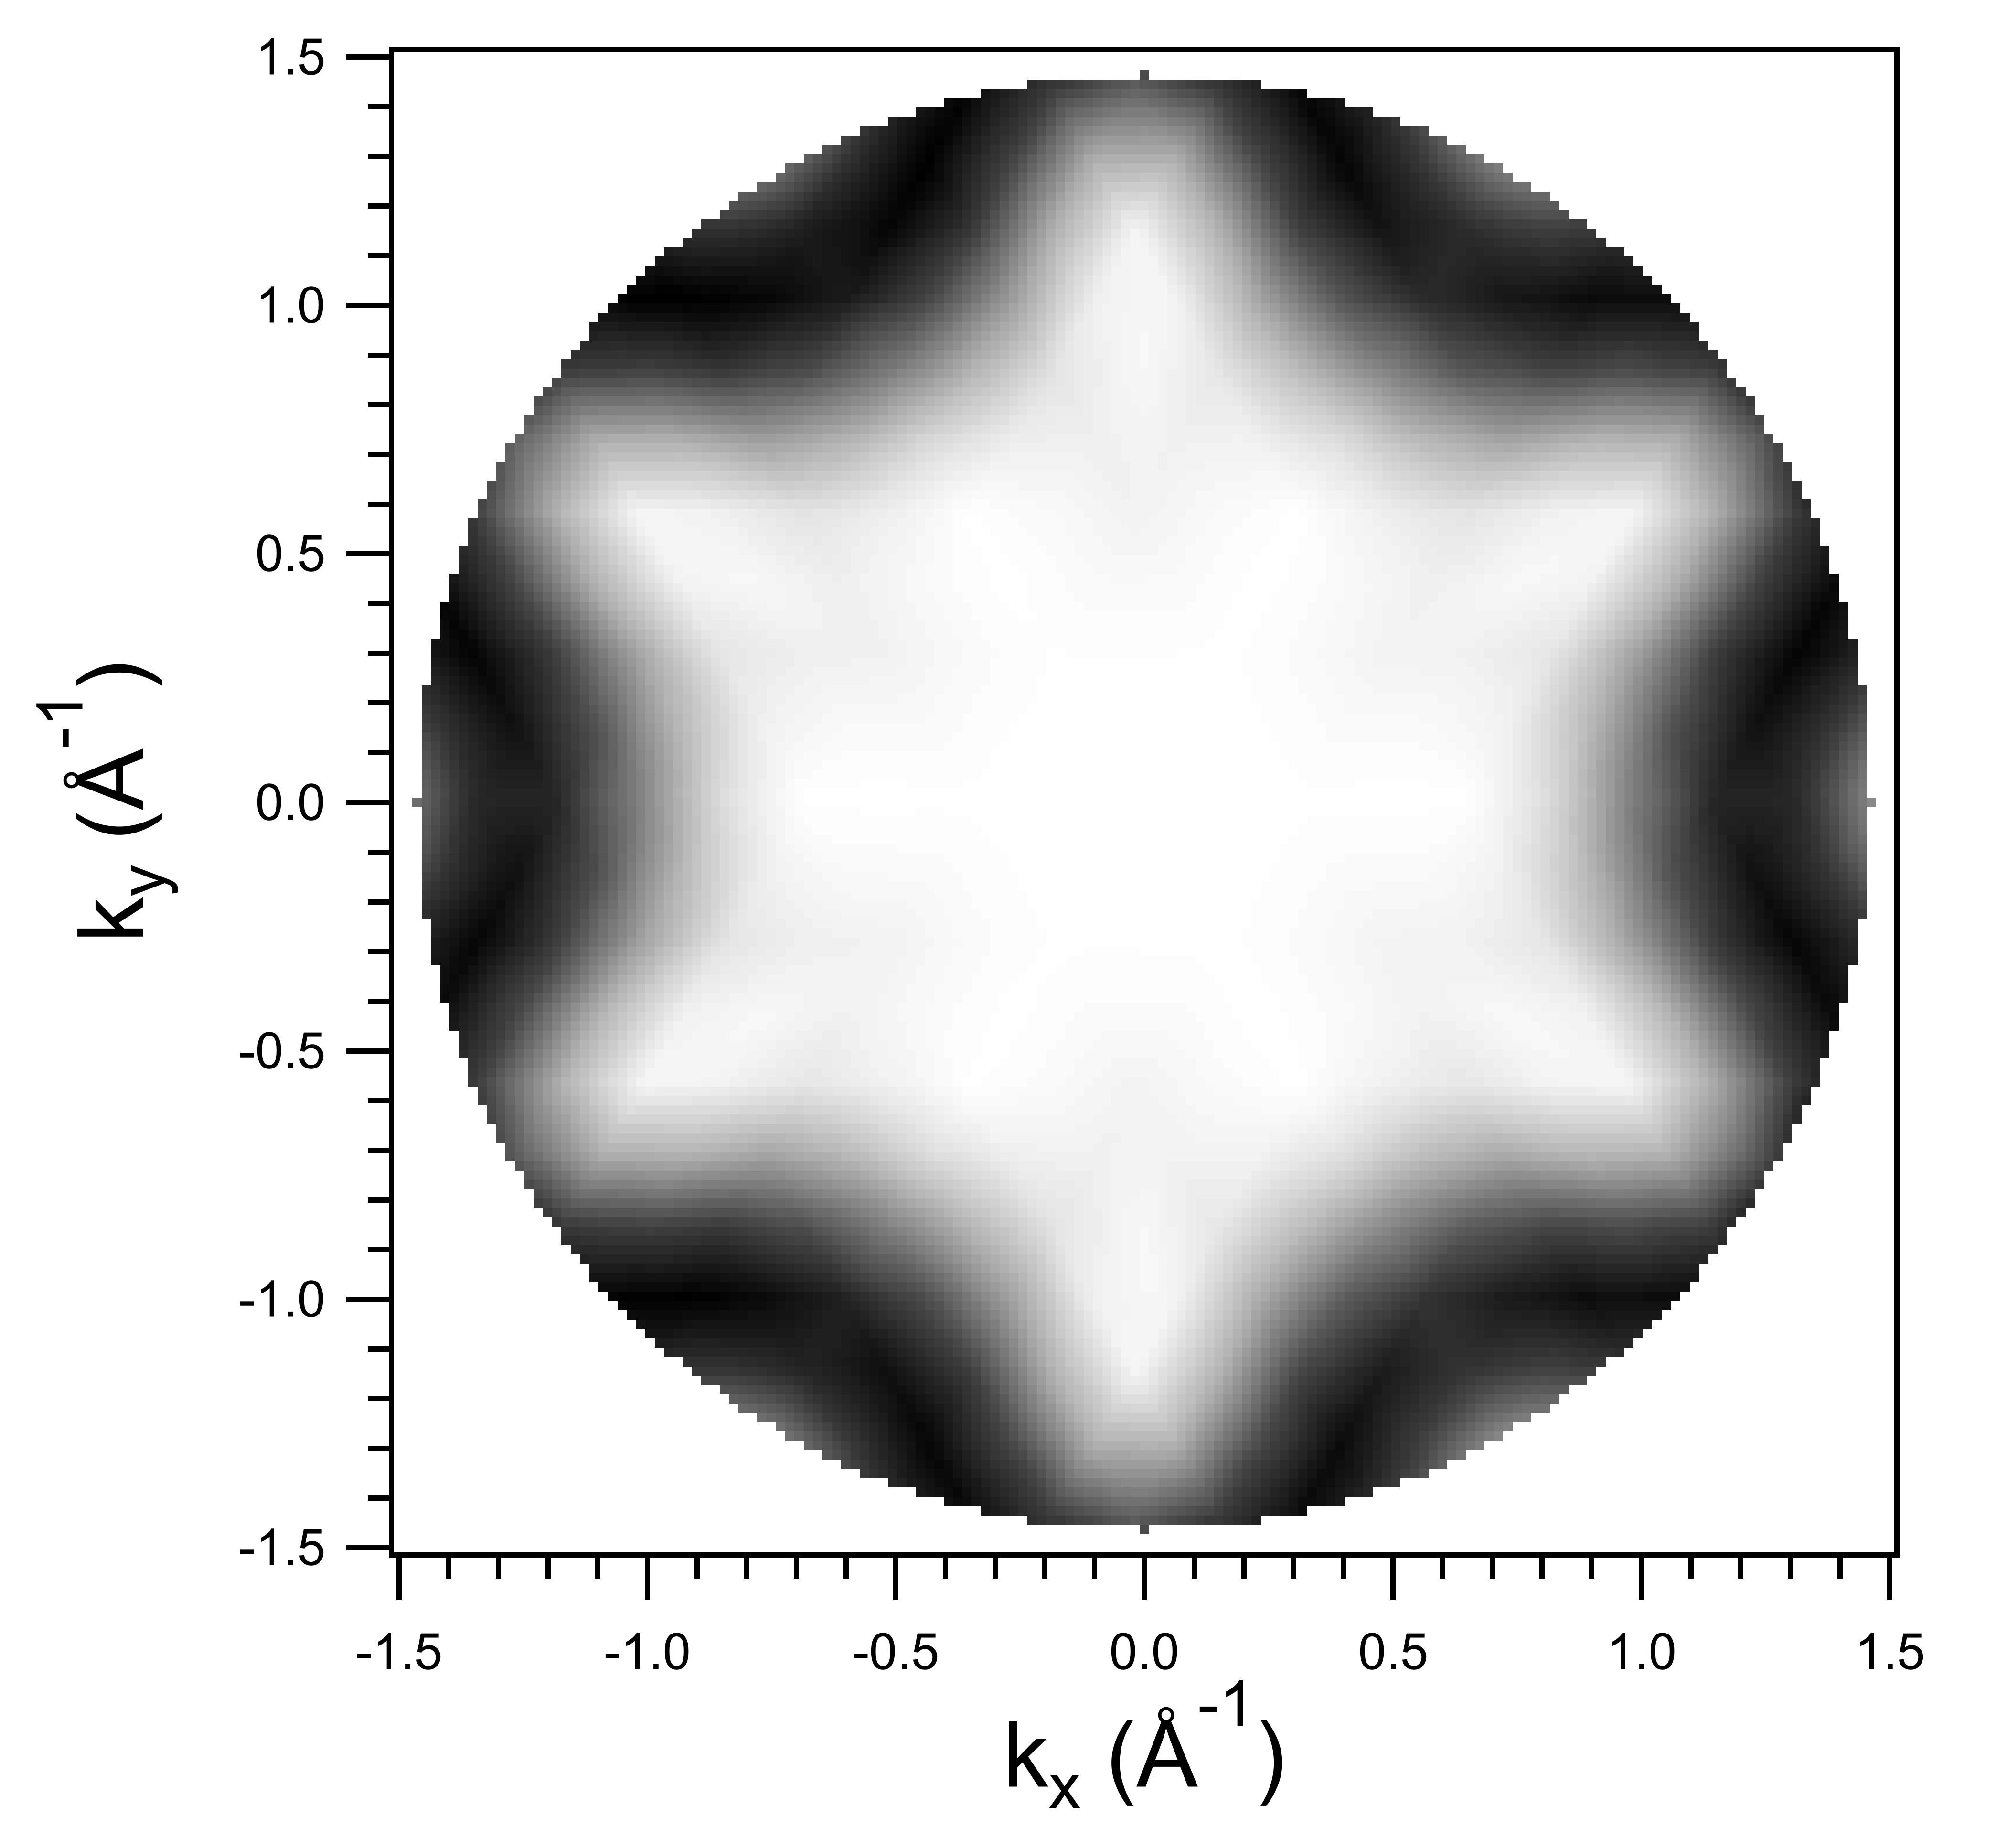
\includegraphics[height=5cm]{./content/pictures/Au+5A/HOMO1_all_CT.pdf}
            %         \subcaption{Theorie Oribtale mit symmetrisierung 2mal um 120 Grad gedreht und zum Ursprungsbild addiert.}
            %     \end{subfigure}
            %     \caption{Zuordnung eines Bildes zu einem der Molekülorbitale.}
            % \end{figure}
            % \begin{figure}
            %     \centering
            %     \begin{subfigure}{0.48\textwidth}
            %         \centering
            %         \includegraphics[height=5cm]{./content/pictures/Au+5A/IMAGE_2021_06_17_007_BE2_65.pdf}
            %         \subcaption{Gemmesen, symmetrisiertes Bild bei einer Bindungsenergie von \SI{2.65}{\electronvolt}.}
            %     \end{subfigure}
            %     \begin{subfigure}{0.48\textwidth}
            %         \centering
            %         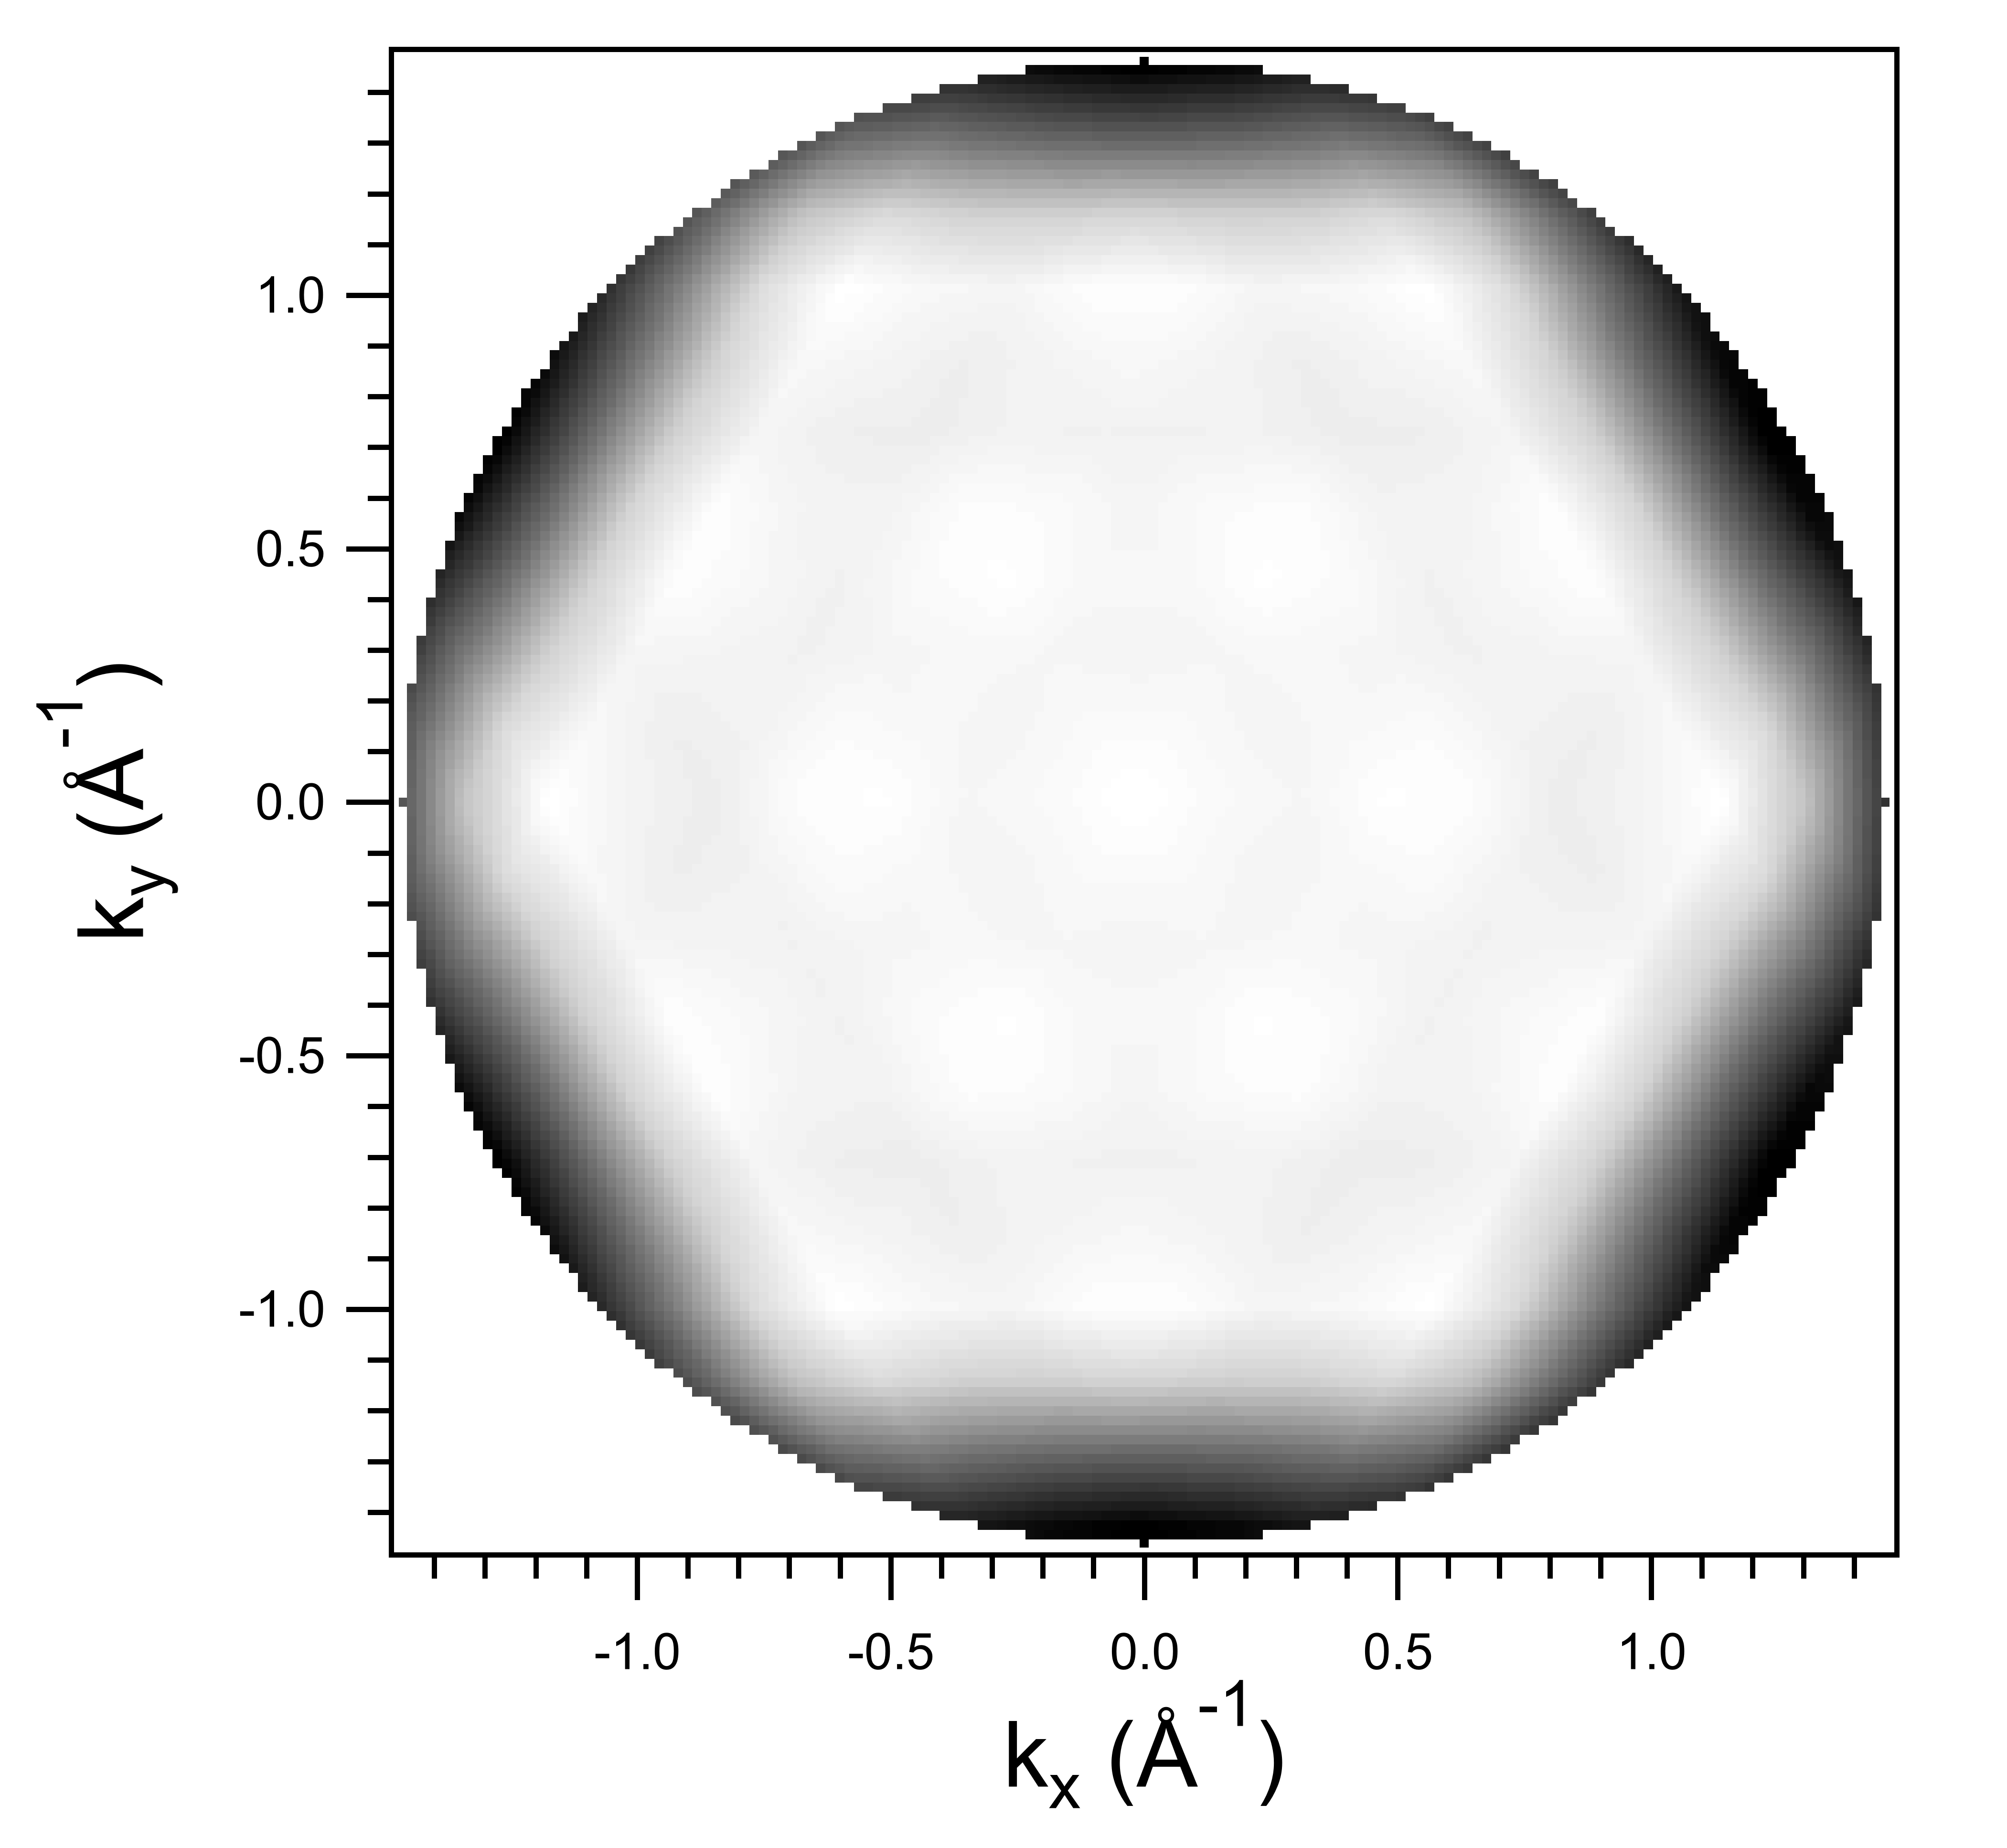
\includegraphics[height=5cm]{./content/pictures/Au+5A/HOMO2_all_CT.pdf}
            %         \subcaption{Theorie Oribtale mit symmetrisierung 2mal um 120 Grad gedreht und zum Ursprungsbild addiert.}
            %     \end{subfigure}
            %     \caption{Zuordnung eines Bildes zu einem der Molekülorbitale.}
            % \end{figure}
        \subsection{5A auf NiO}
                Die Abwesenheit sehr ausgeprägter Merkmale in den impulsaufgelösten Bildern bestätigt die Annahme aus \autoref{sec:Praep}, dass sich die Moleküle auf der Oberfläche nicht regelmäßig anordnen.
                Auch wenn sich in den integrierten Spektren in \autoref{fig:NiO_Filmdicke} klar zeigt, dass sich bei einigen Energien die Intensität erhöht ist in den entsprechenden Bildern keine klare Zuordnung möglich.

        \subsection{FeO}
            \begin{figure}
                \centering
                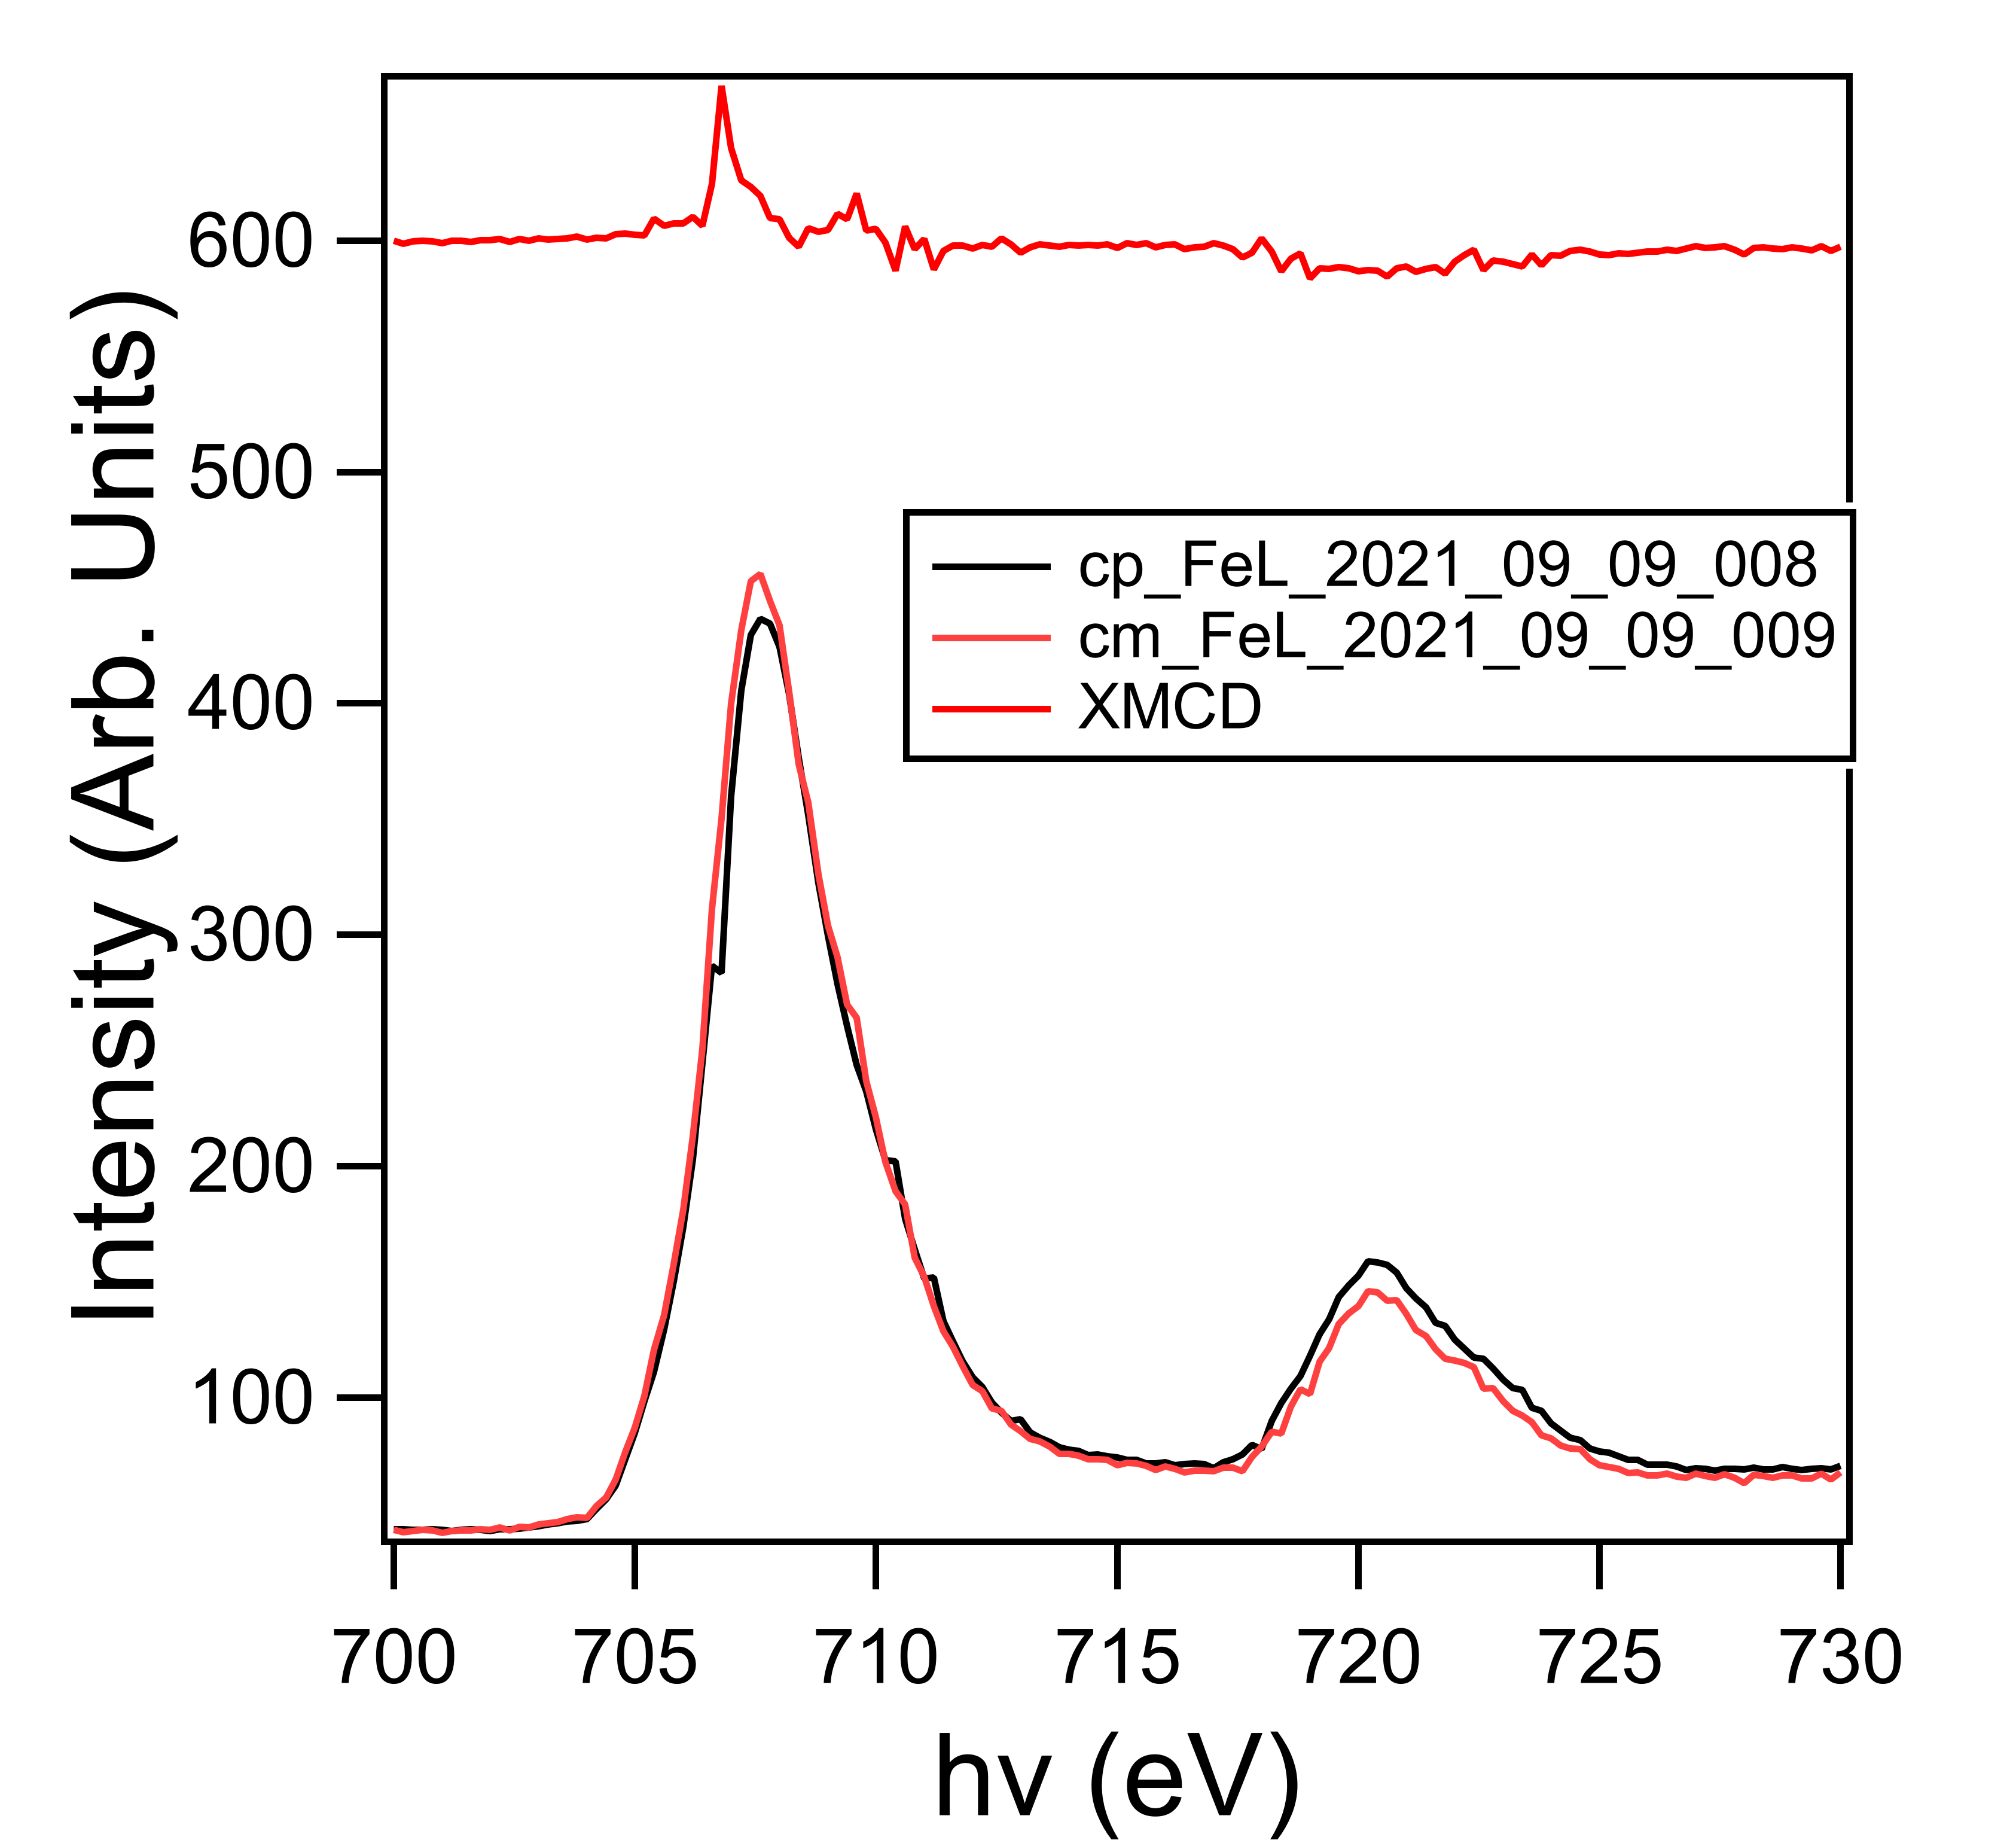
\includegraphics[width=0.7\textwidth]{./content/pictures/FeO/XMCD.png}
                \caption{XAS Spektren für links- und rechtzirkular polarisiertes Licht und ihre Differenz.}
                \label{fig:XMCD}
            \end{figure}
            \begin{figure}
                \centering
                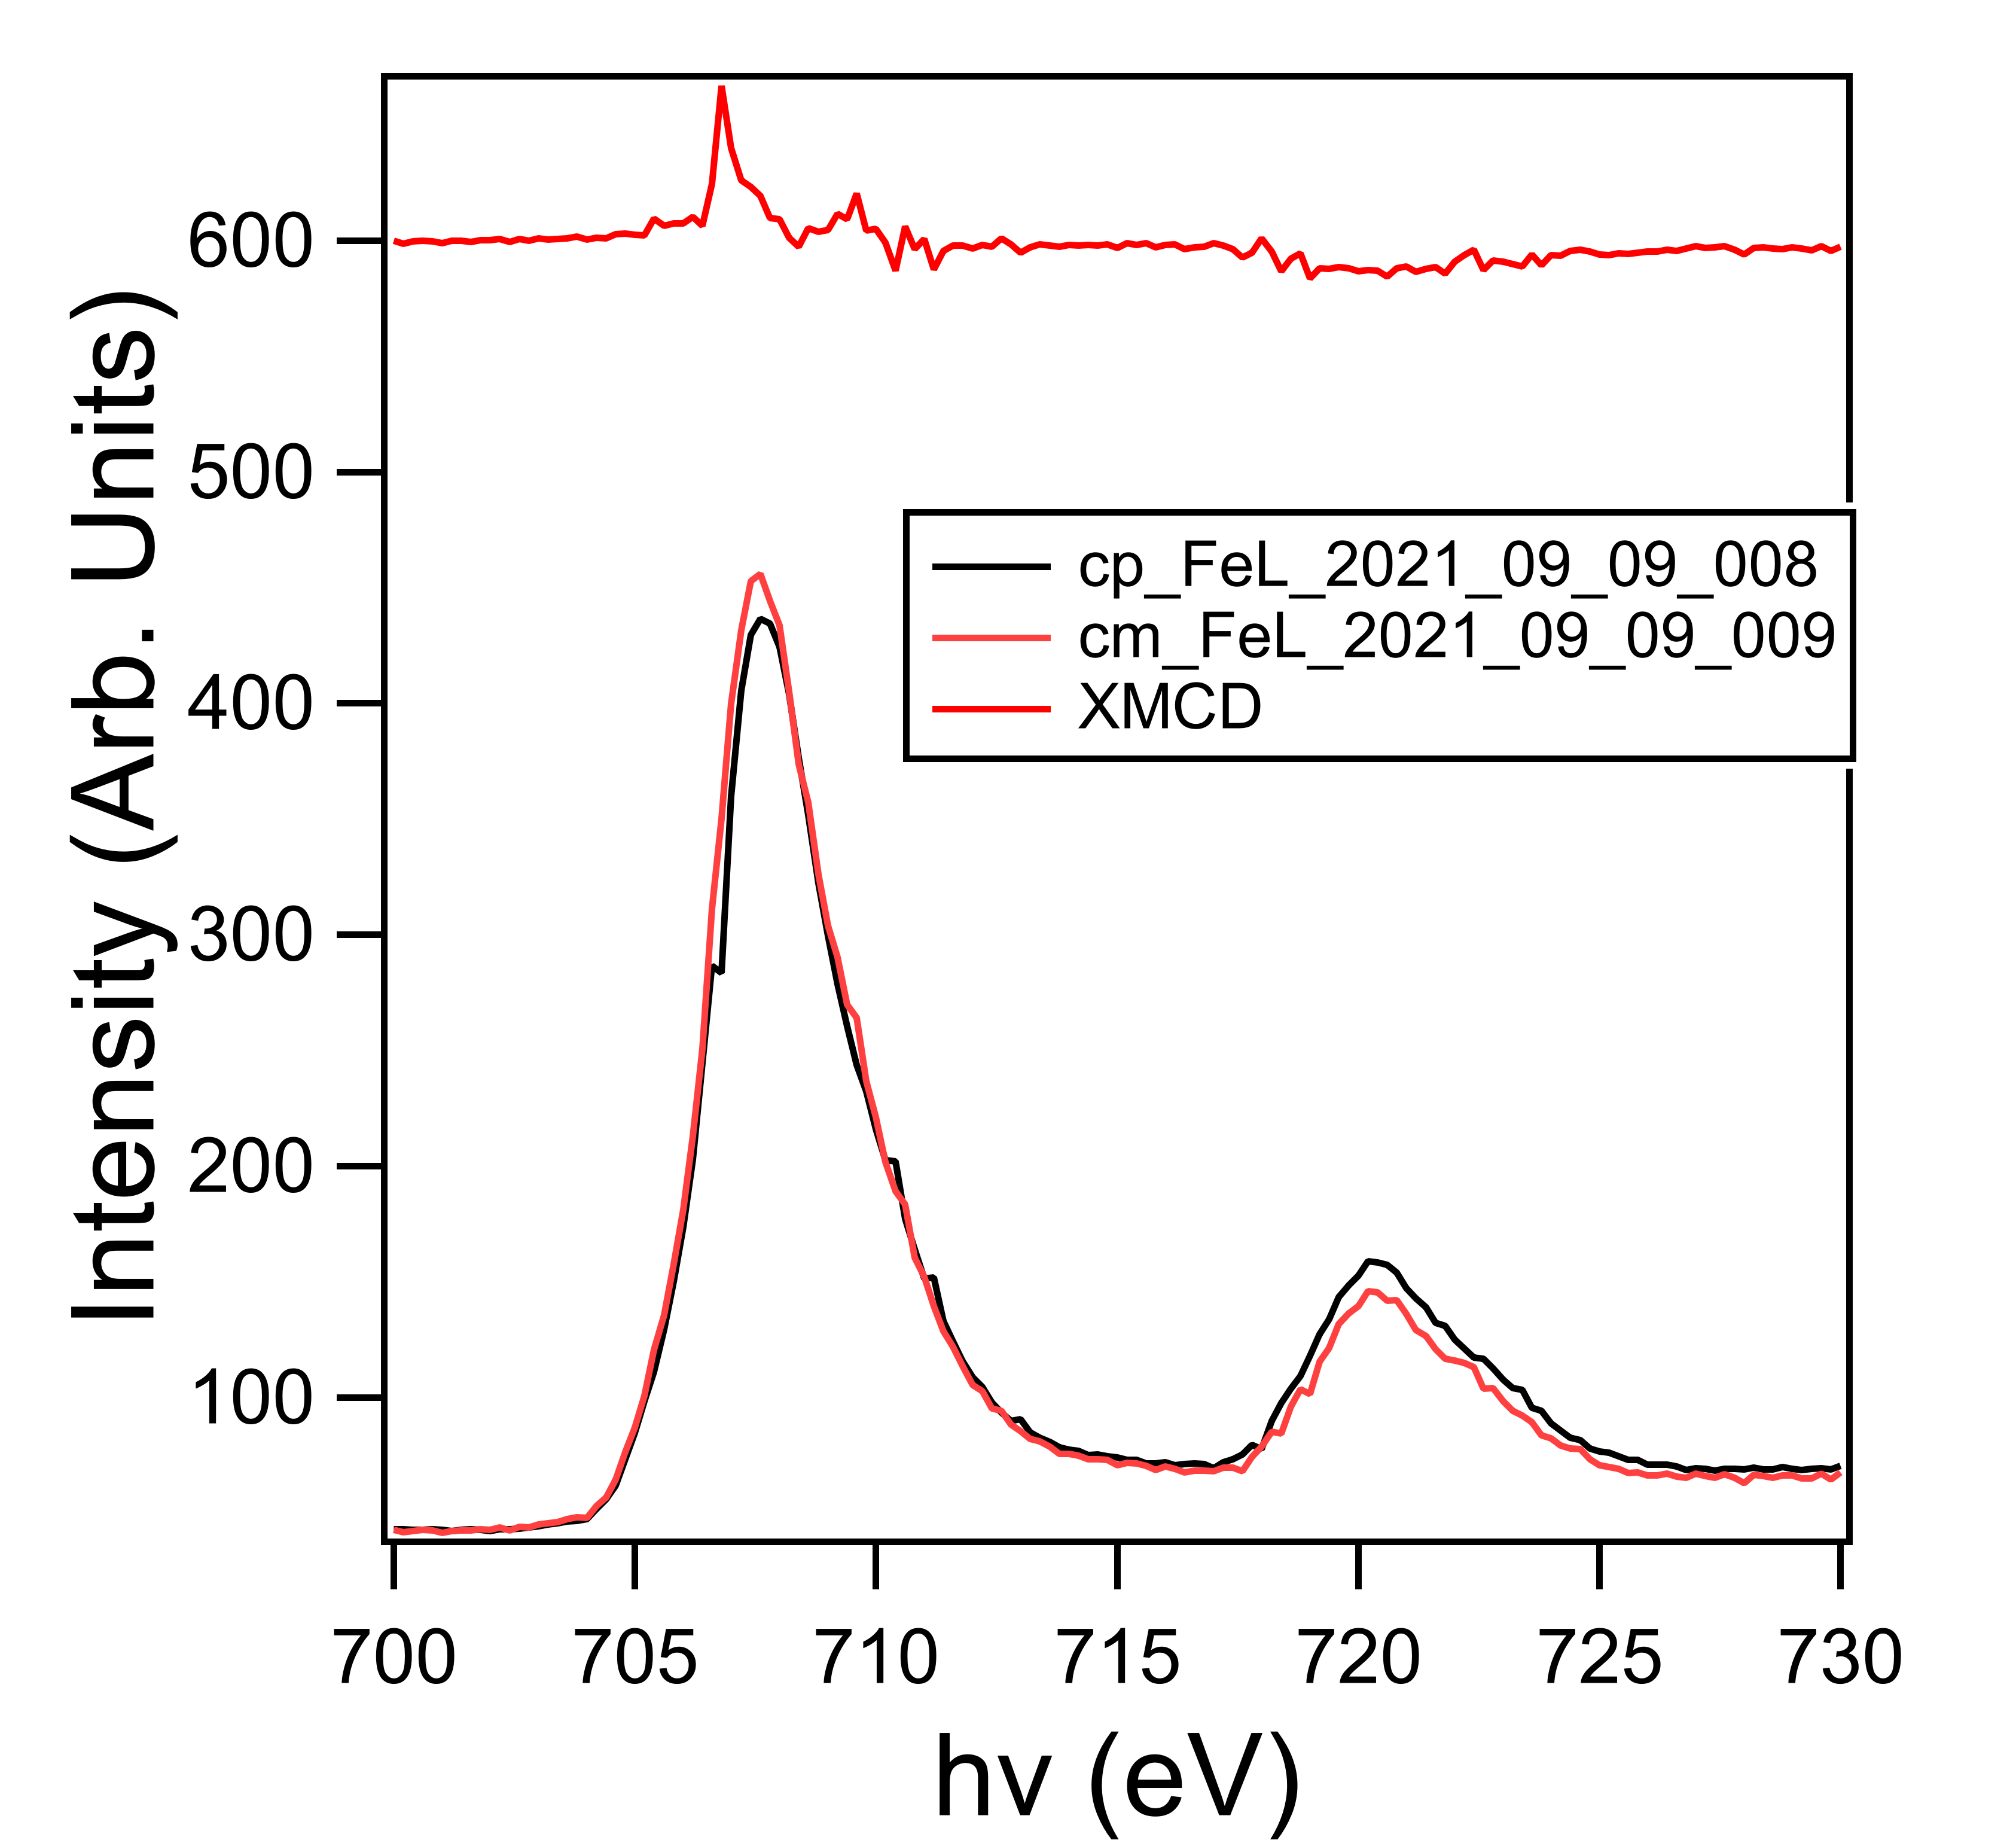
\includegraphics[width=0.7\textwidth]{./content/pictures/FeO/XMCD.png}
                \caption{XAS Spektren für s- und p- polarisiertes Licht, sowie dessen Differenz.}
                \label{fig:XMLD}
            \end{figure}
            \begin{figure}
                \centering
                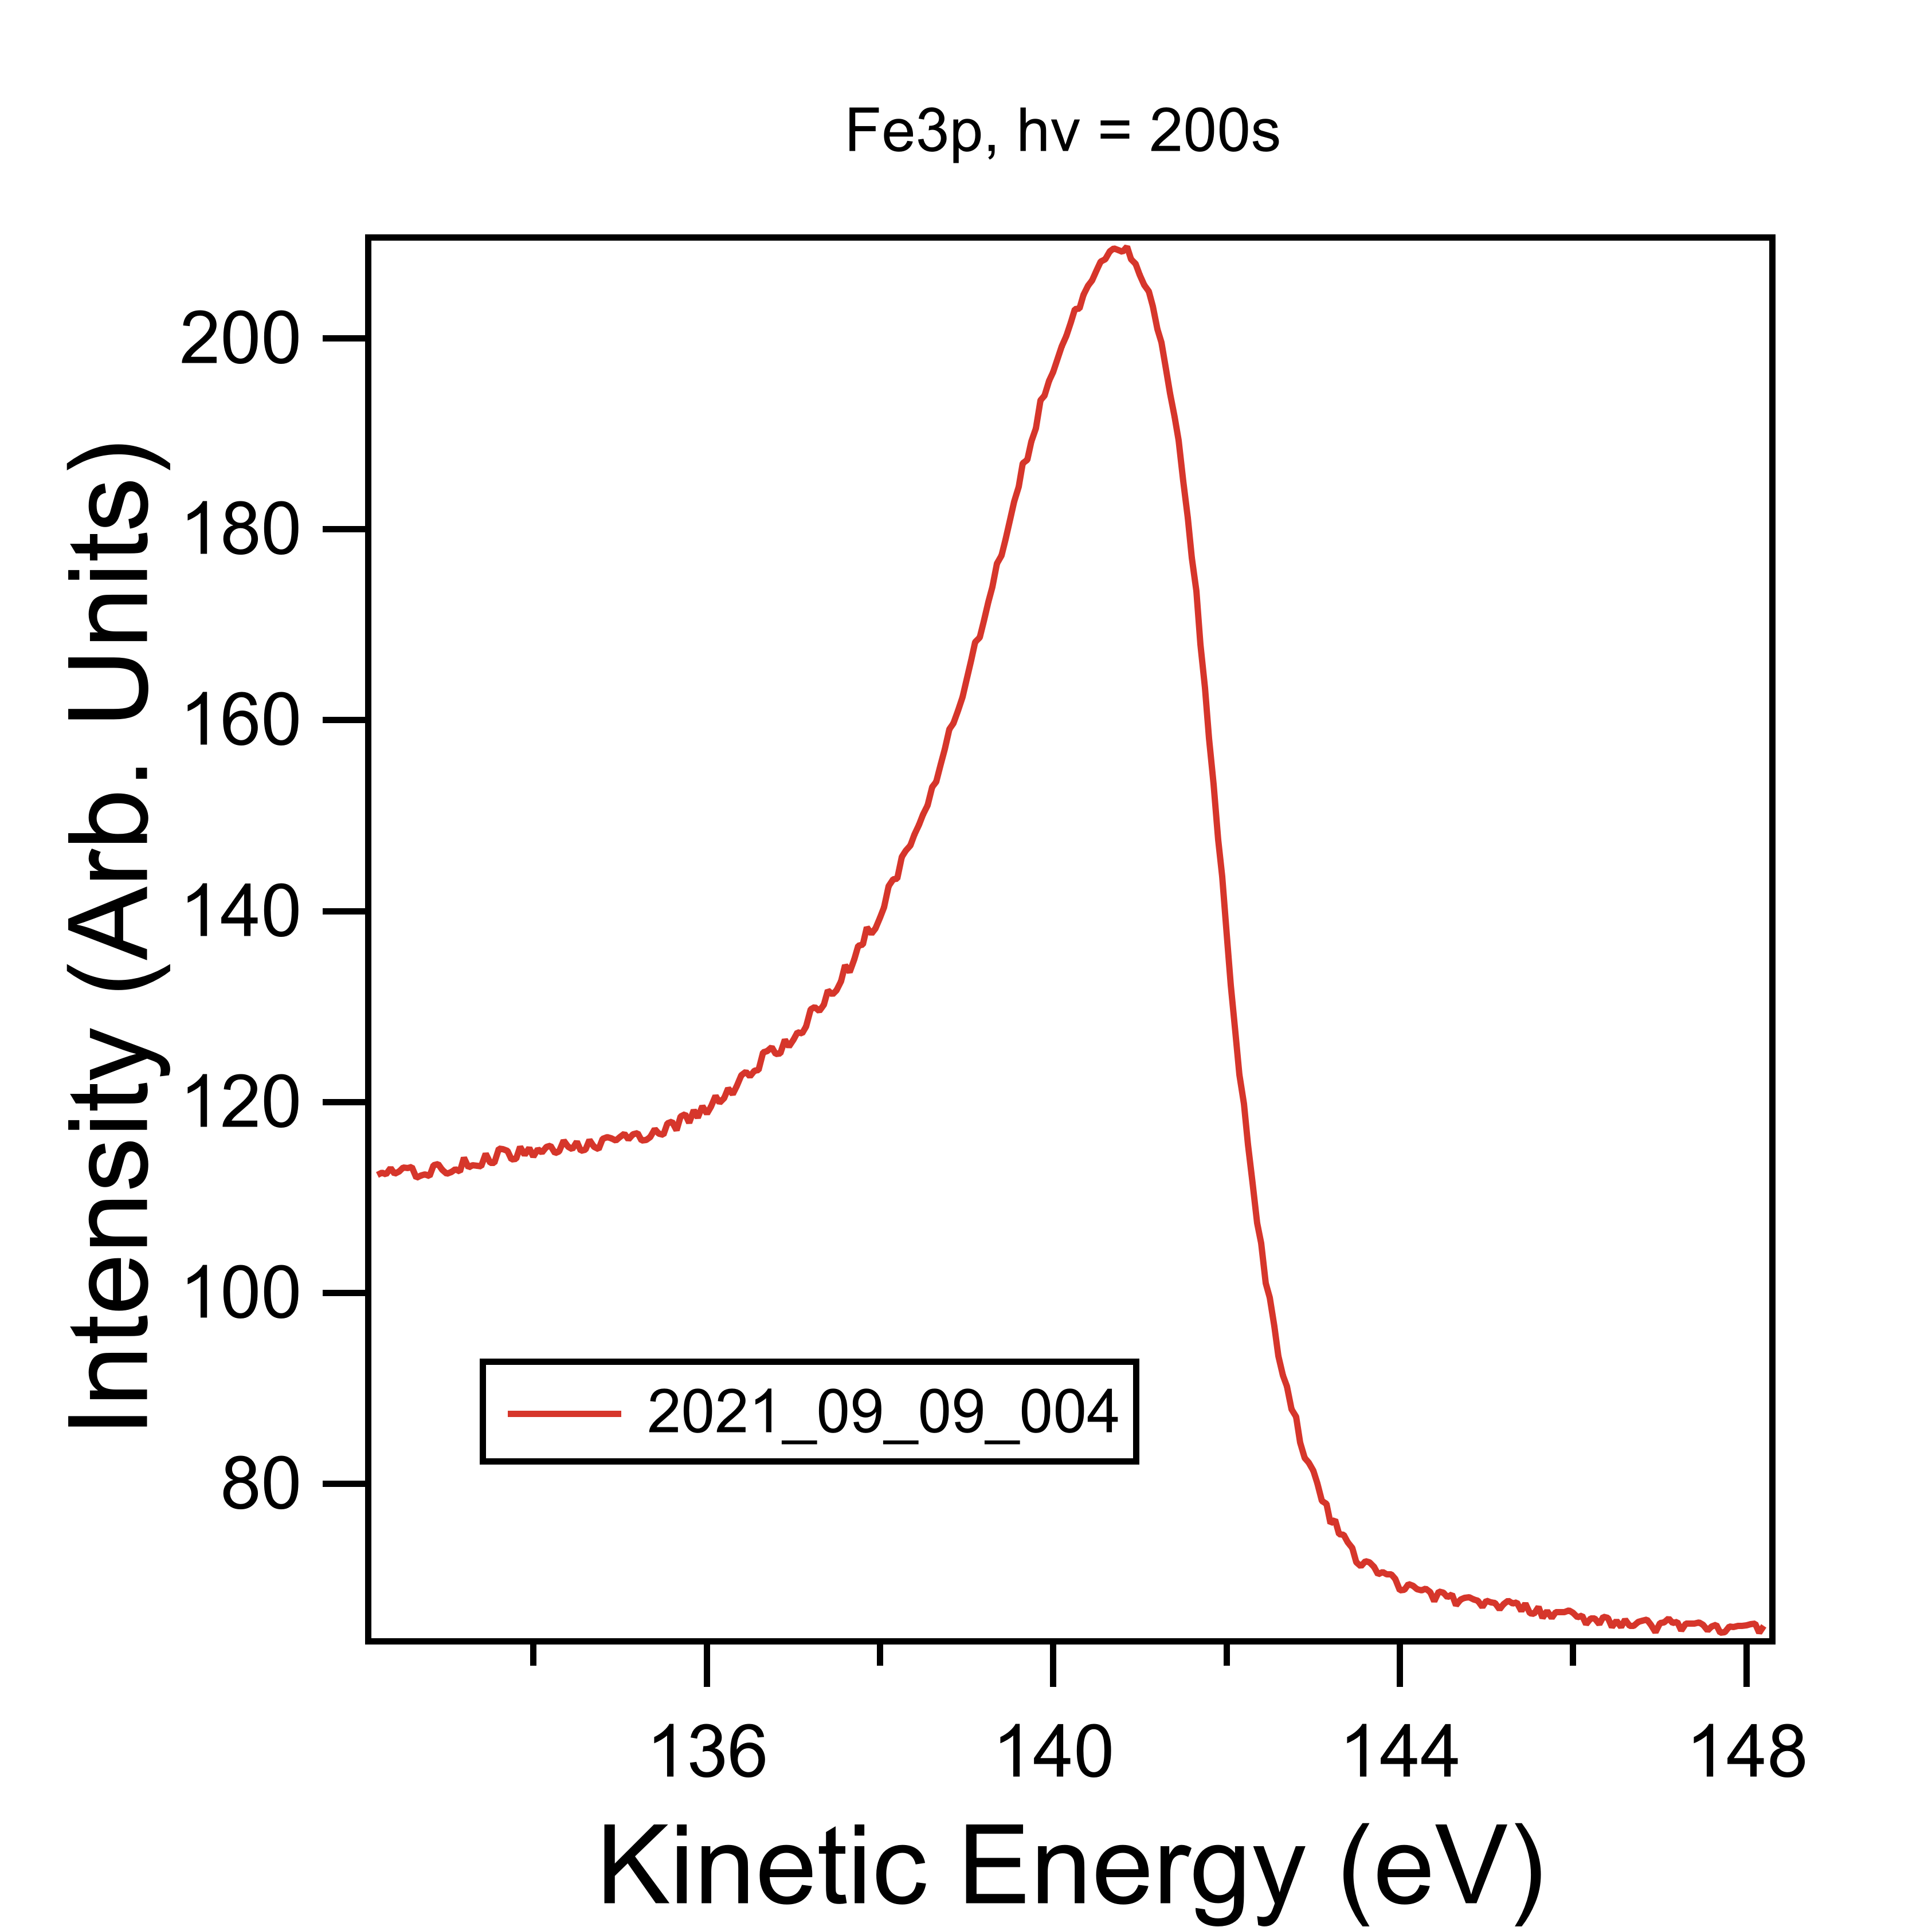
\includegraphics[width=0.7\textwidth]{./content/pictures/FeO/XPS_Fe3p.png}
                \caption{XPS Spektrum des $\ce{Fe}_{3\text{p}}$ Übergang.}
                \label{fig:XPSFe3p}
            \end{figure}


        \subsection{5A auf FeO}
                Im Widerspruch zu den Interpretation aus \autoref{sec:Praep} wo das nicht Vorhandensein die Interpretation zulies, dass sich die Moleküle nicht auf der Oberfläche ordnen sind in den Tomographiebildern merkmale von Molekülen zu erkennen.
                Diese Merkmale können sich nur ausbilden, wenn sich die Moleküle regelmäßig und in gleicher Orientierung anordnen.
                Anderenfalls würden sich die Photoemissionströme überlagern und es gäbe verschwommene Bilder.
                \begin{figure}
                    \centering
                    \begin{subfigure}[t]{0.48\textwidth}
                        \centering
                        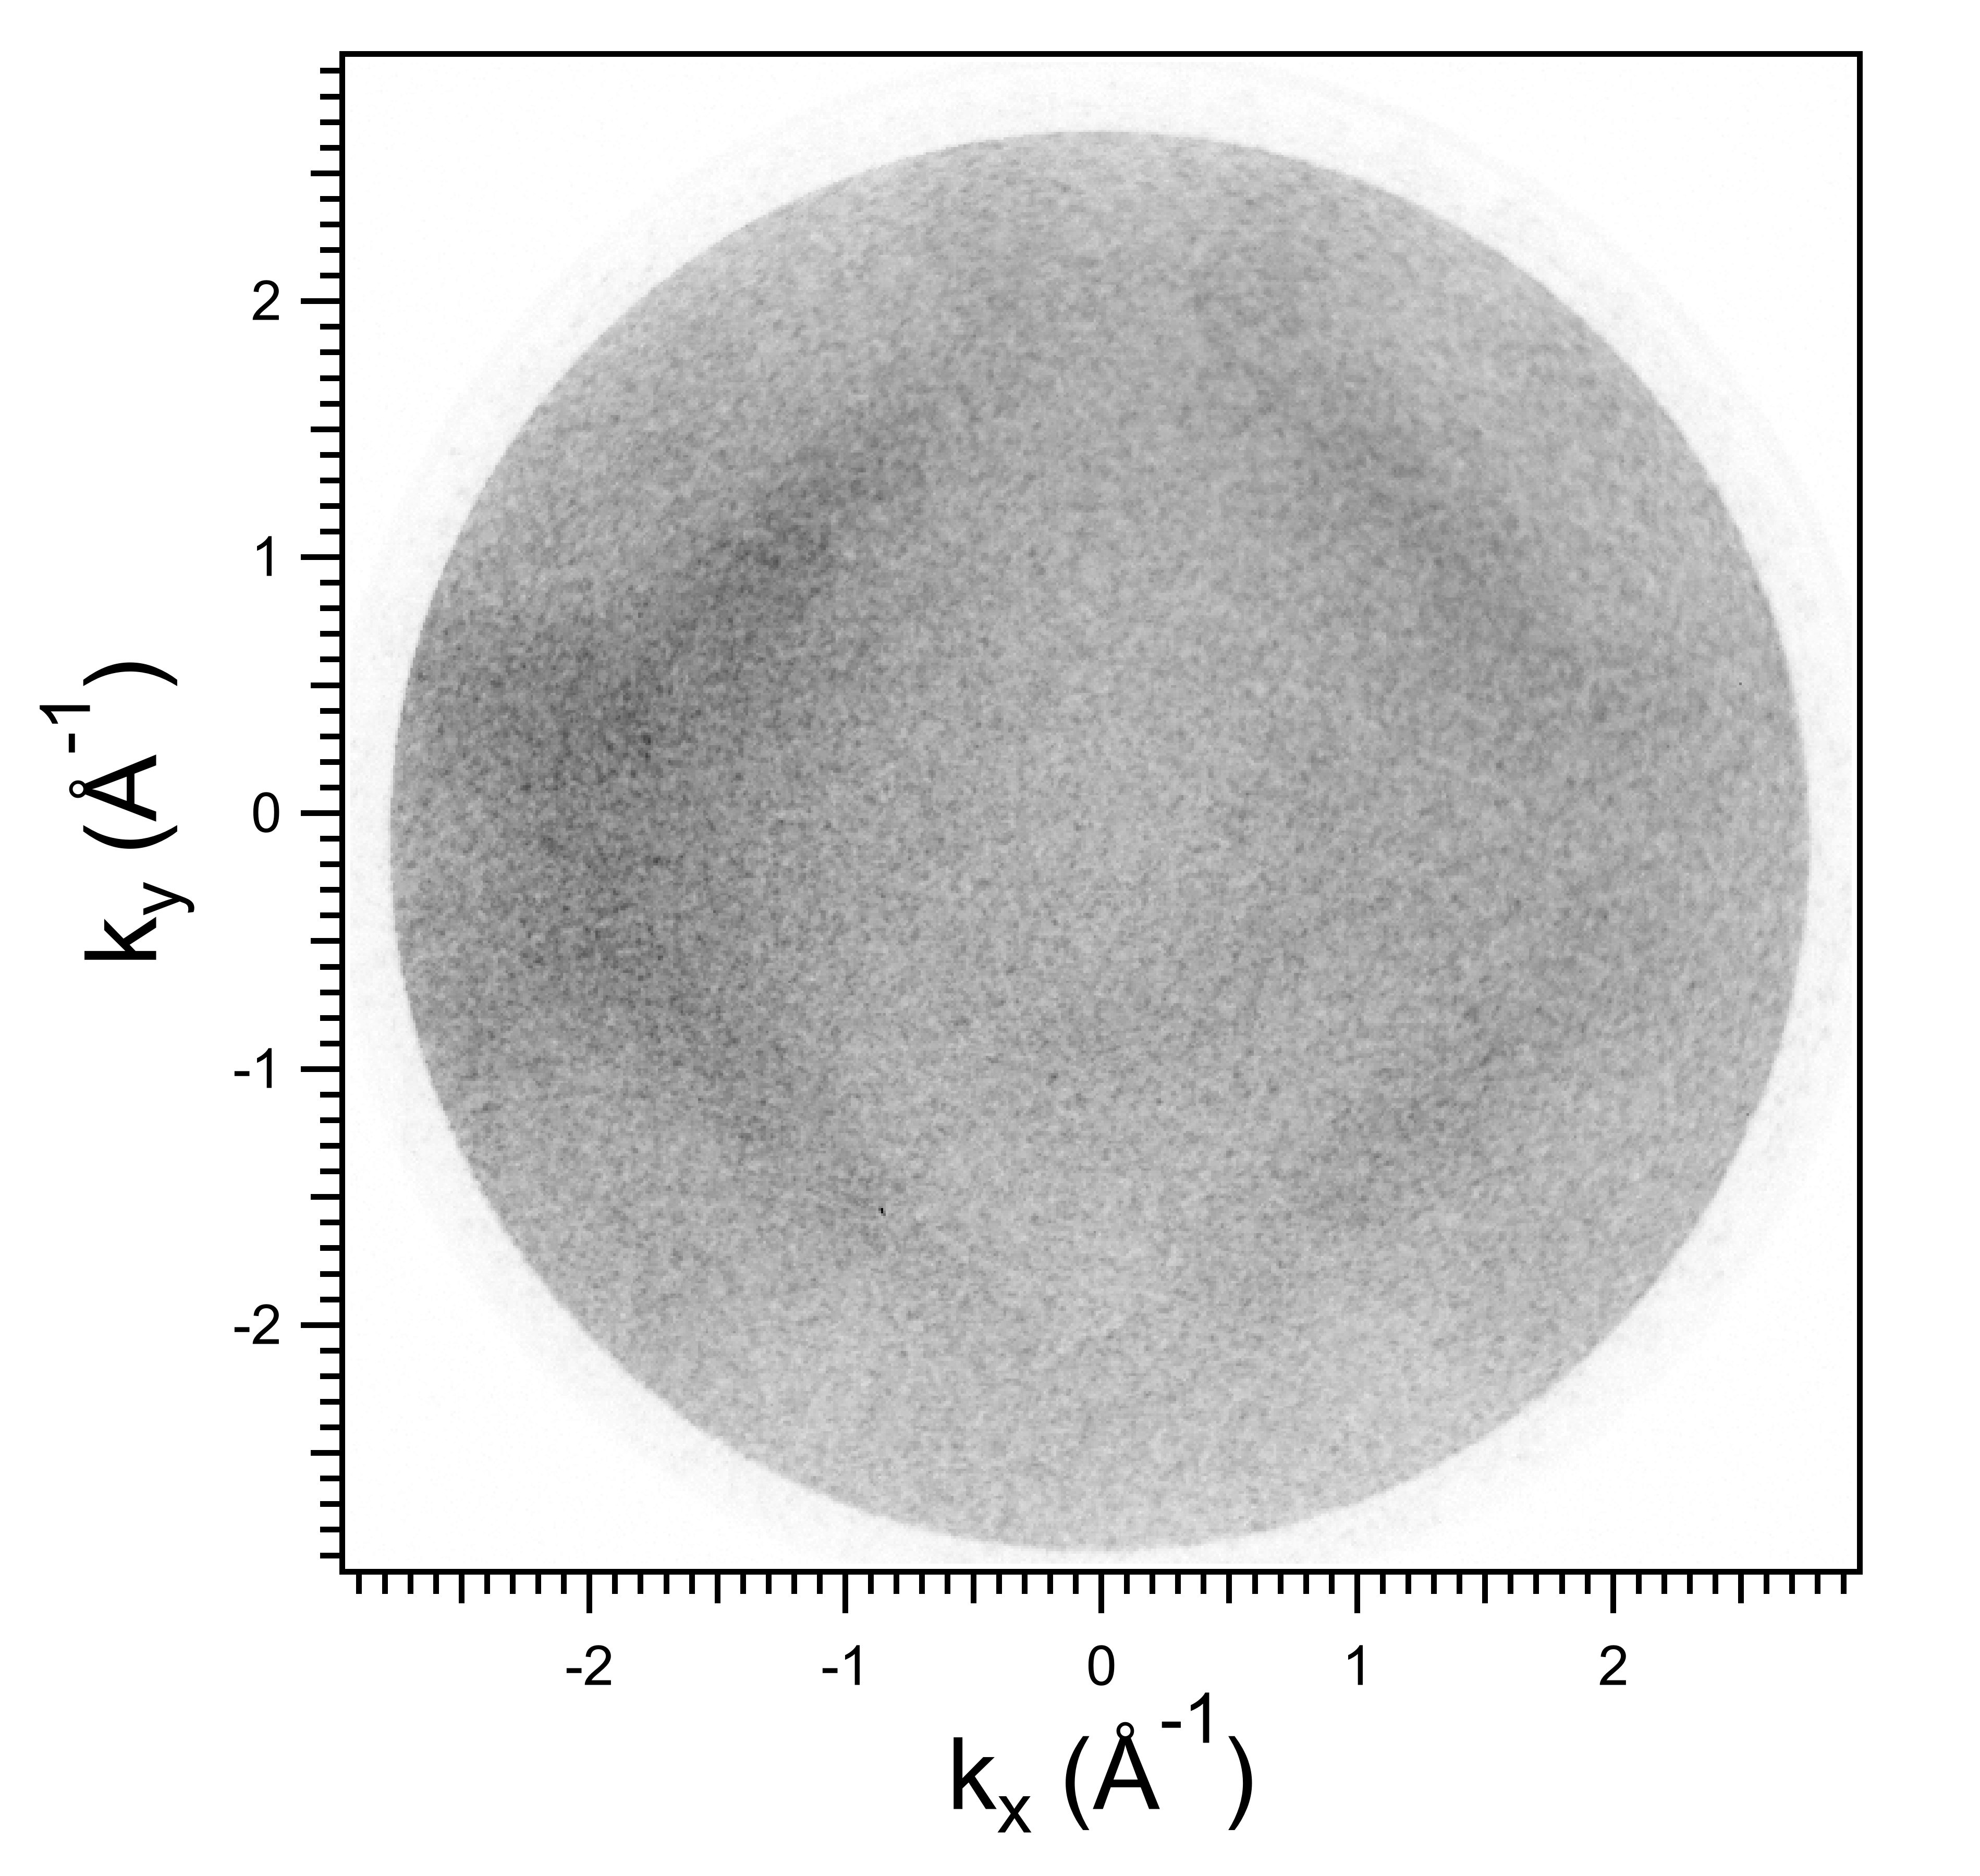
\includegraphics[height=5cm]{./content/pictures/FeO+5A/FeO_5A_34_80eV.png}
                        \subcaption{Das Bild für eine kinetische Energie von \SI{34.80}{\electronvolt}.}
                    \end{subfigure}
                    \begin{subfigure}[t]{0.48\textwidth}
                        \centering
                        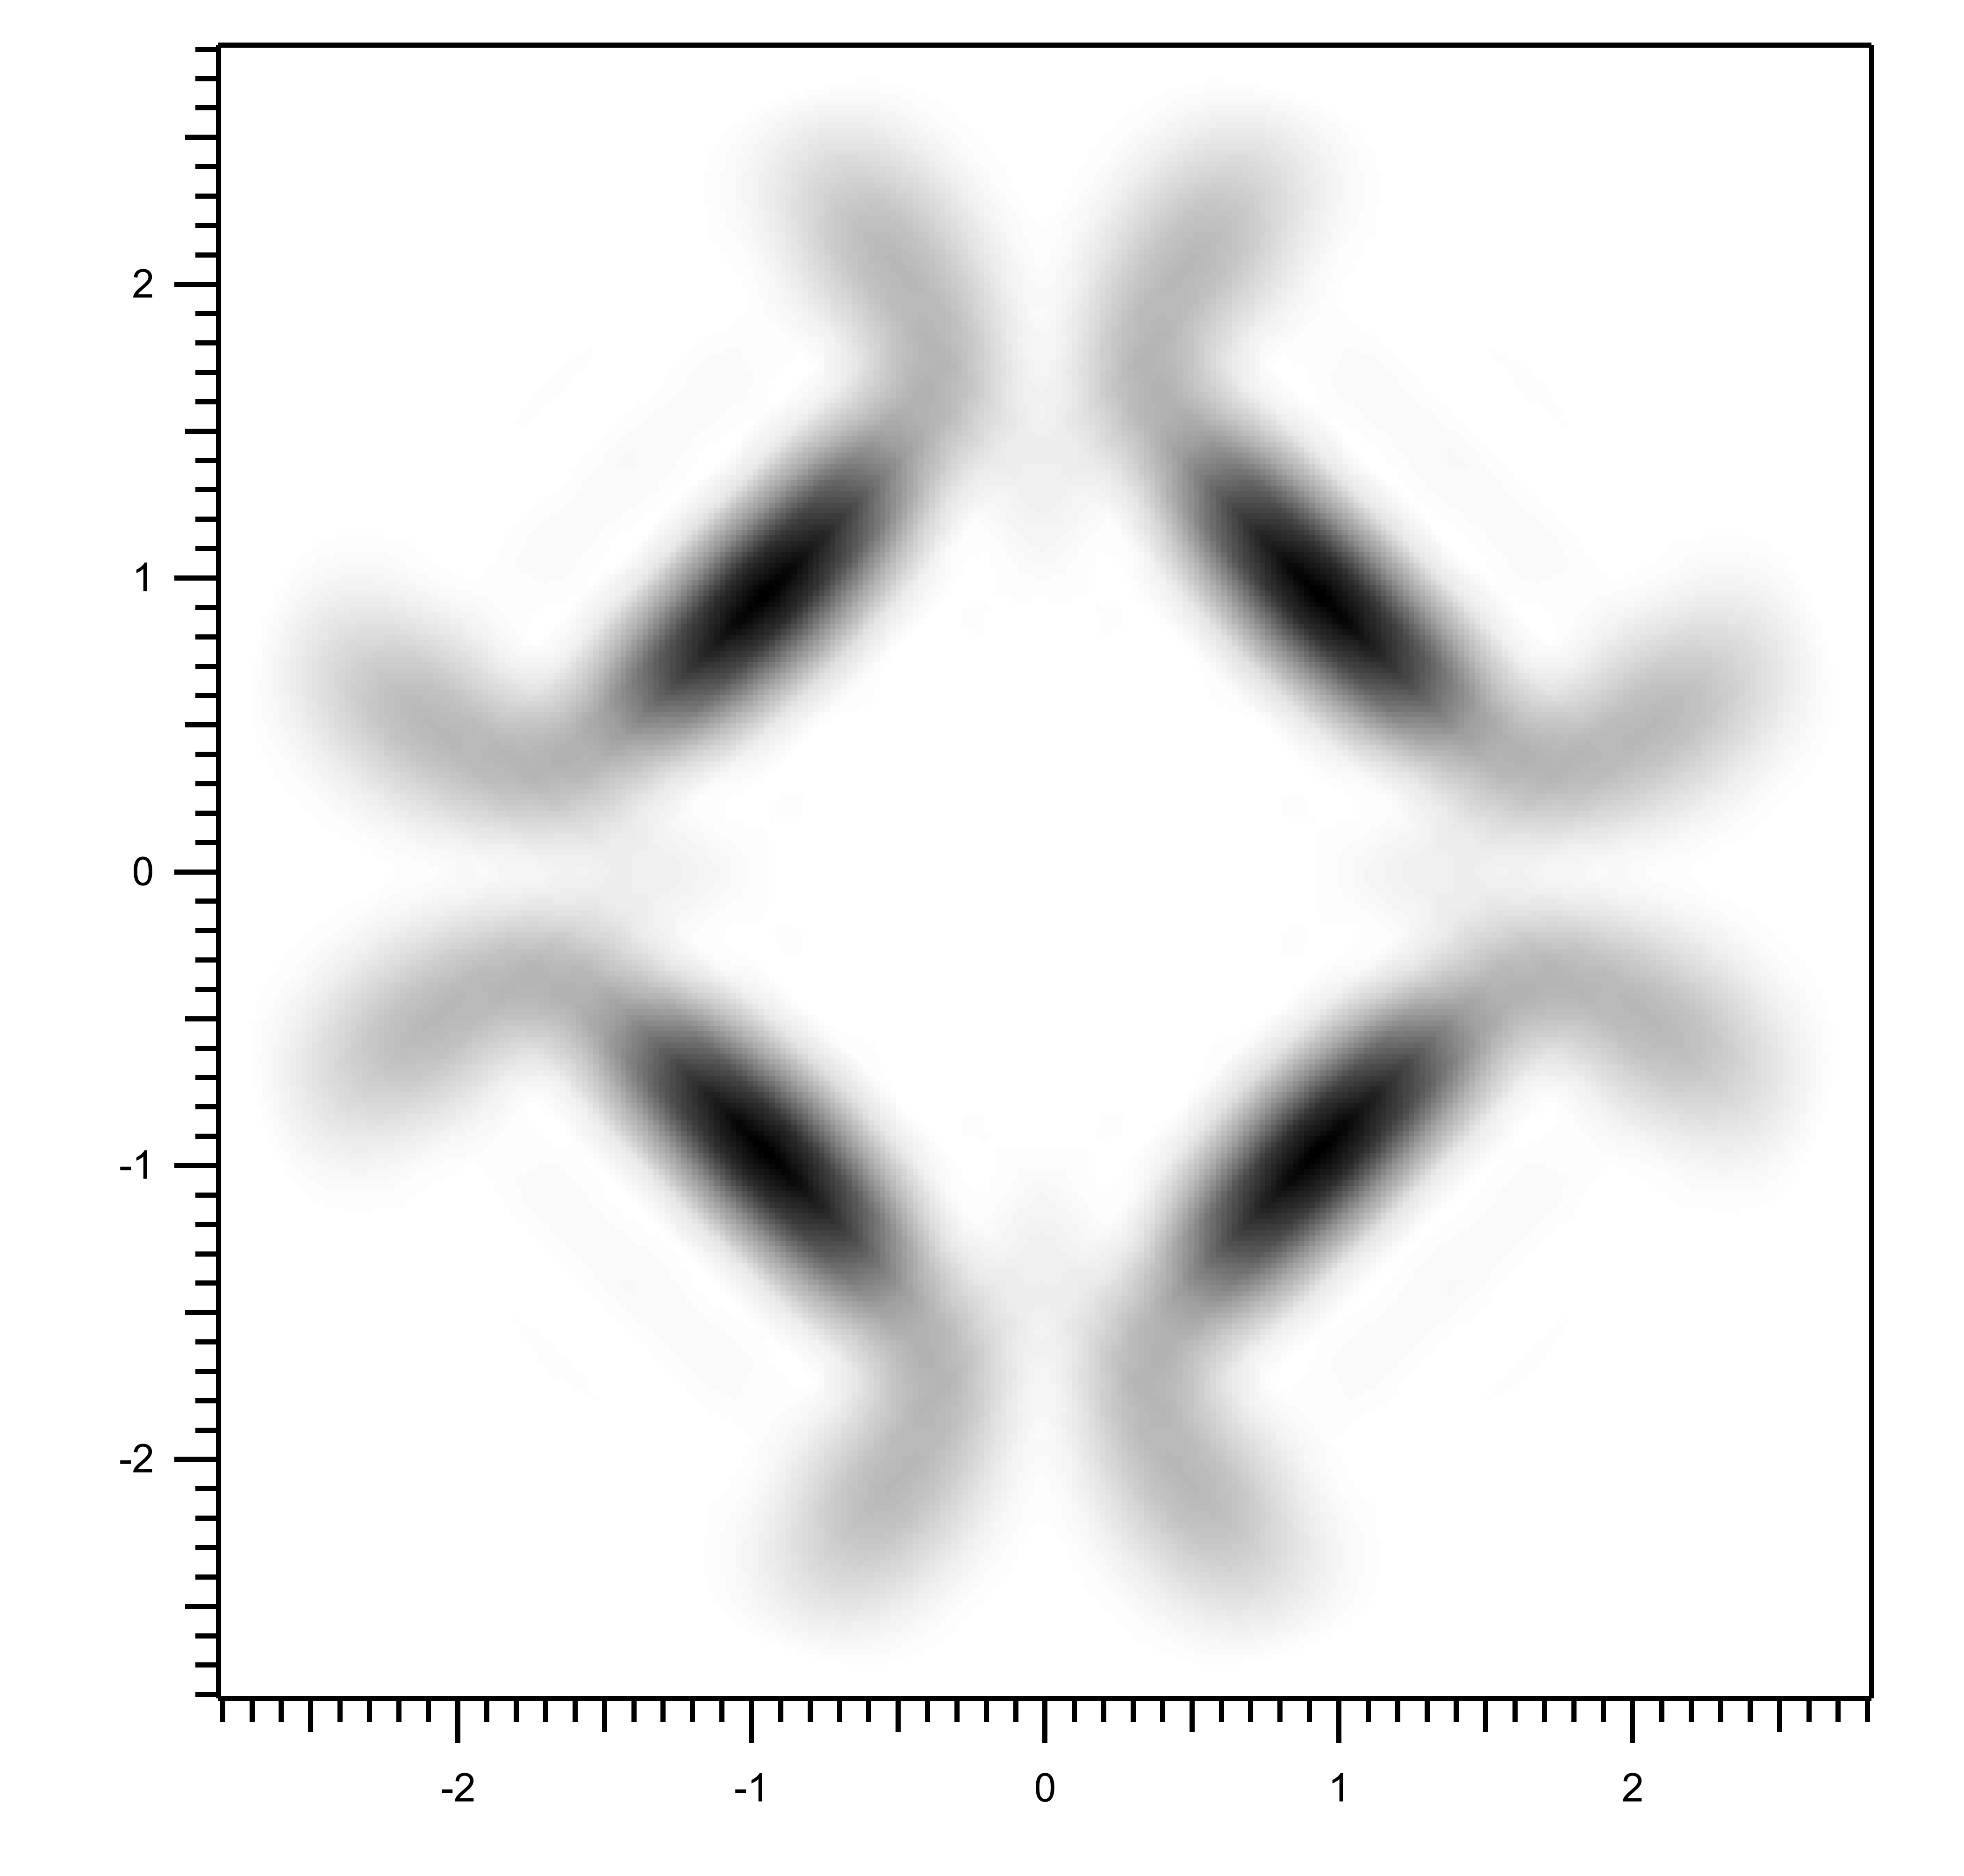
\includegraphics[height=5cm]{./content/pictures/FeO+5A/MO_LUMO_RT_RT.png}
                        \subcaption{Das LUMO mit Symmetrisierung zweier um \SI{90}{\degree} verdrehten Übergitter.}
                    \end{subfigure}
                    \caption{Vergleich der gemessenen Intensitätsverteilung mit der des symmetrisierten LUMO.}
                    \label{fig:FeO5A1}
                \end{figure}
                \begin{figure}
                    \centering
                    \begin{subfigure}[t]{0.48\textwidth}
                        \centering
                        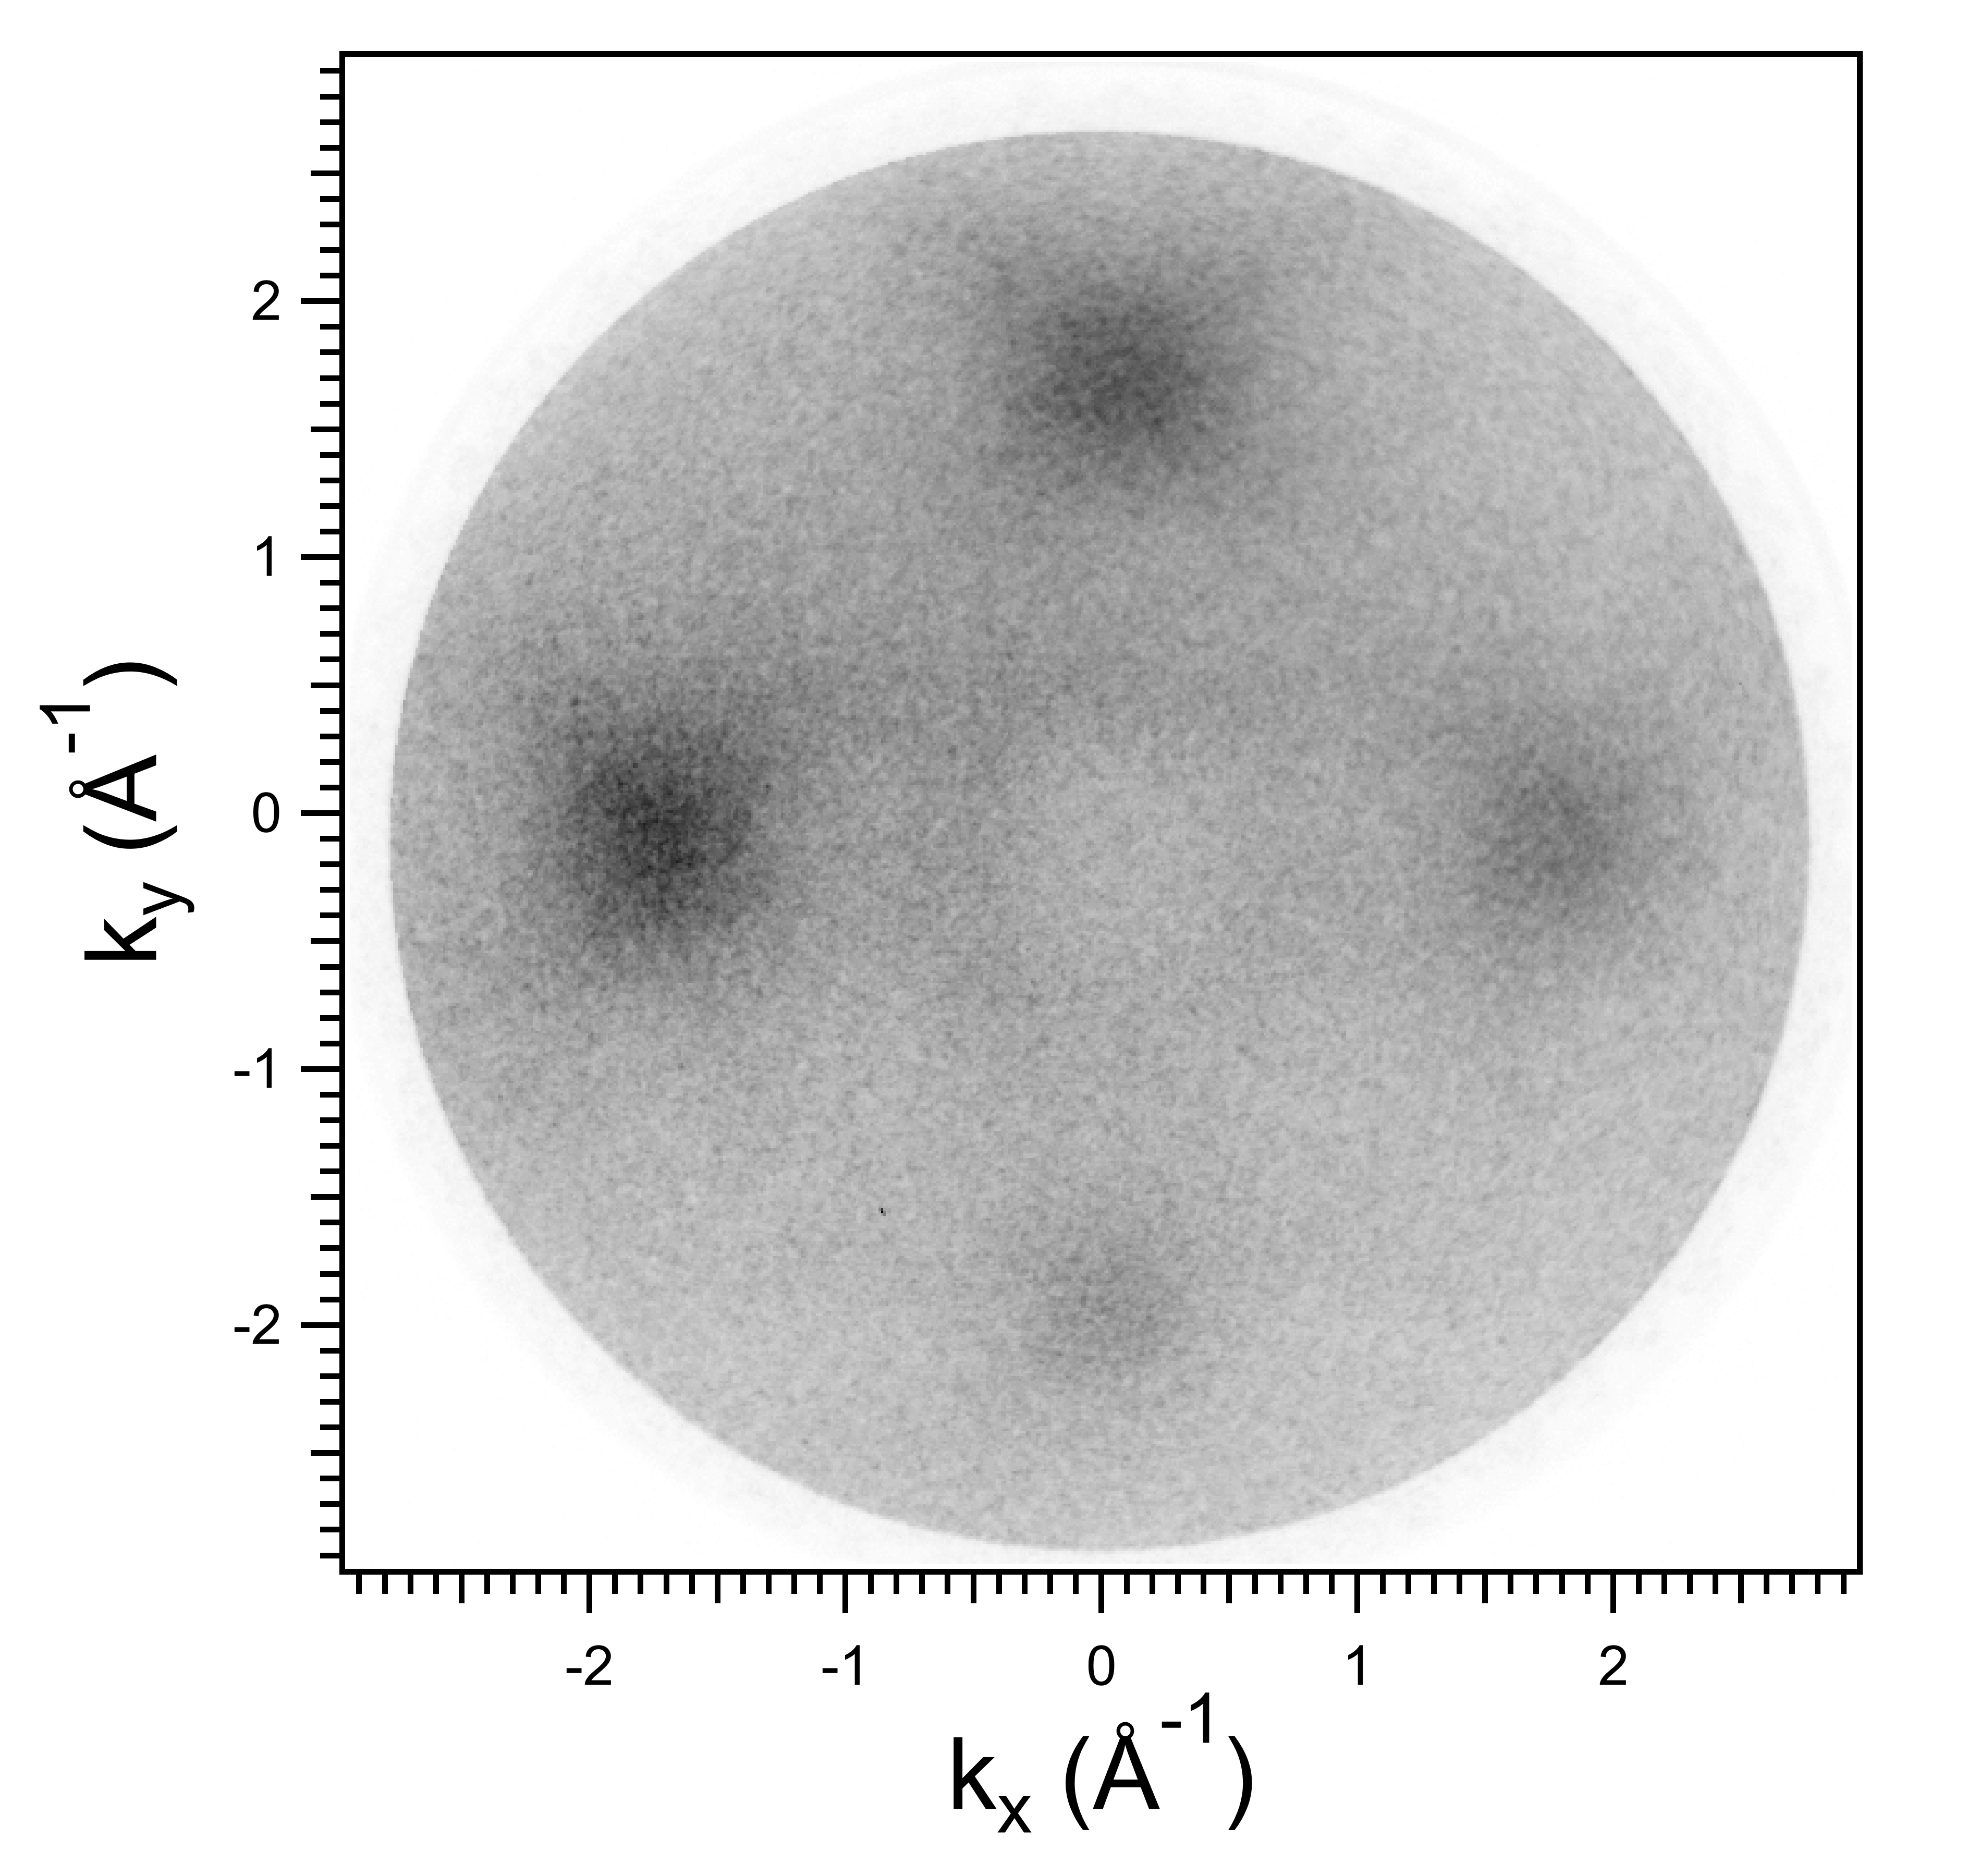
\includegraphics[height=5cm]{./content/pictures/FeO+5A/FeO_5A_33_75eV.png}
                        \subcaption{Das Bild für eine kinetische Energie von \SI{33.75}{\electronvolt}.}
                    \end{subfigure}
                    \begin{subfigure}[t]{0.48\textwidth}
                        \centering
                        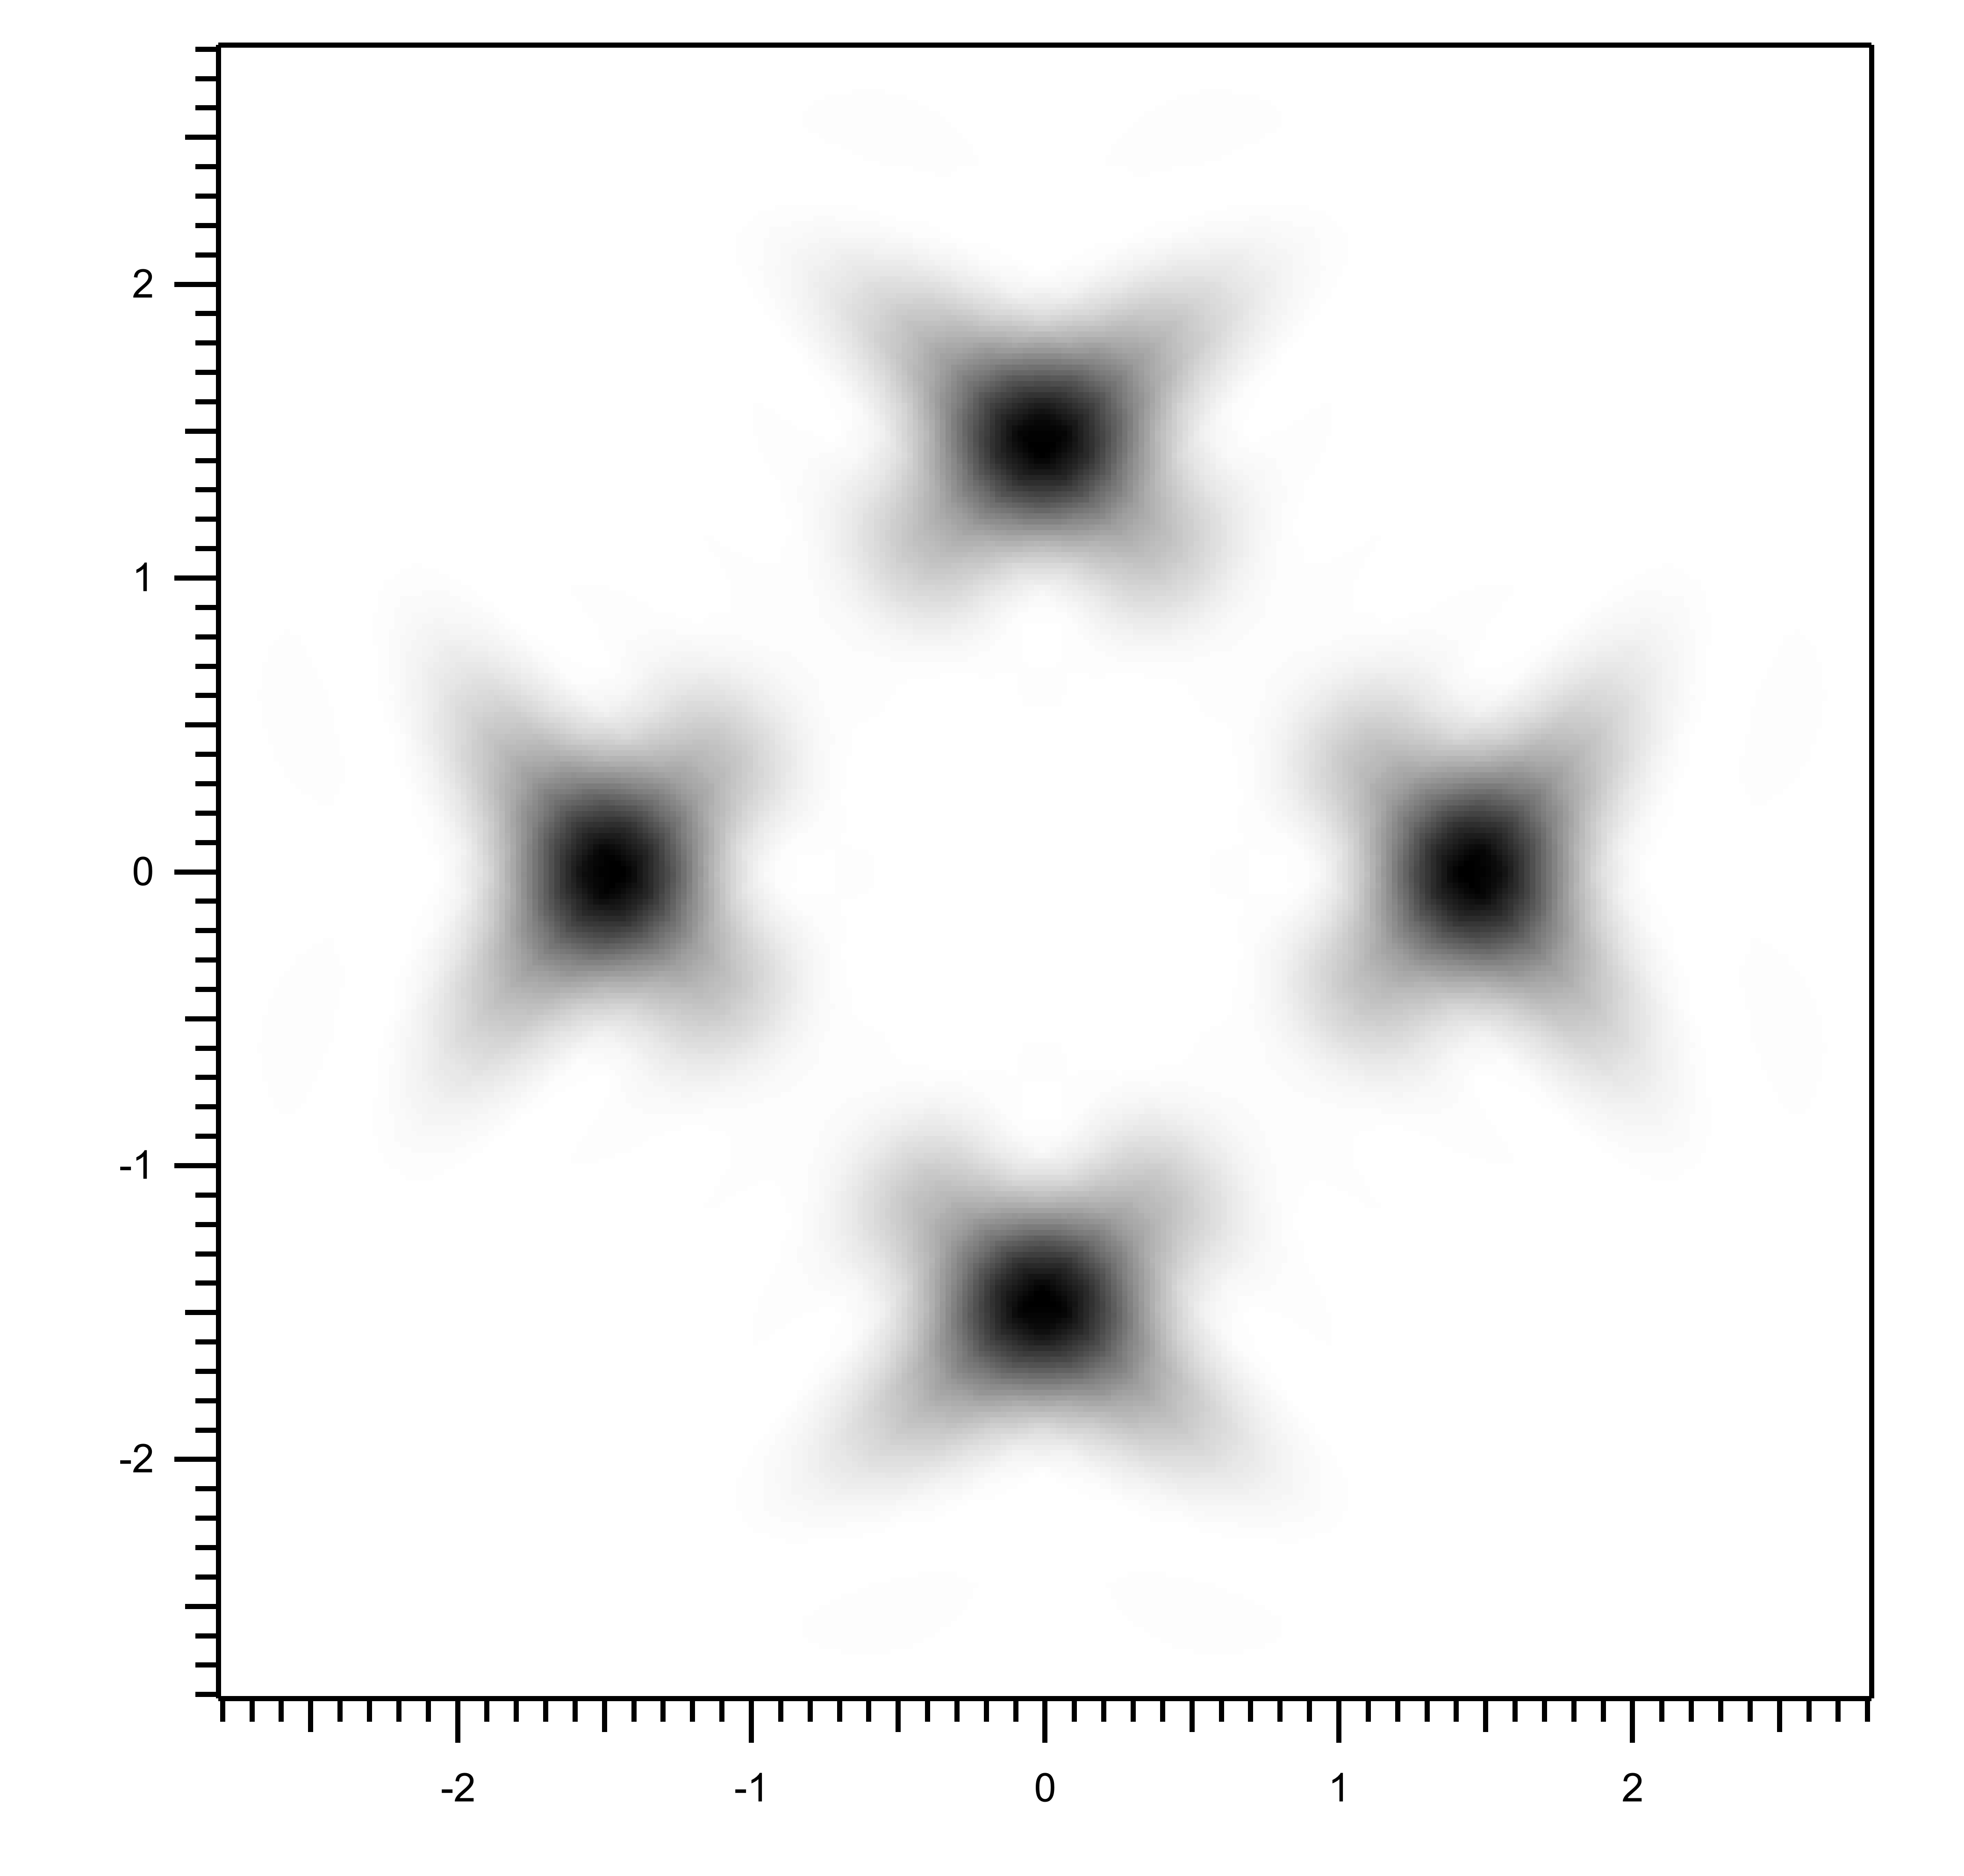
\includegraphics[height=5cm]{./content/pictures/FeO+5A/MO_HOMO_RT_RT.png}
                        \subcaption{Das HOMO mit Symmetrisierung zweier um \SI{90}{\degree} verdrehten Übergitter.}
                    \end{subfigure}
                    \caption{Vergleich der gemessenen Intensitätsverteilung mit der des symmetrisierten HOMO.}
                    \label{fig:FeO5A2}
                \end{figure}
                \begin{figure}
                    \centering
                    \begin{subfigure}[t]{0.48\textwidth}
                        \centering
                        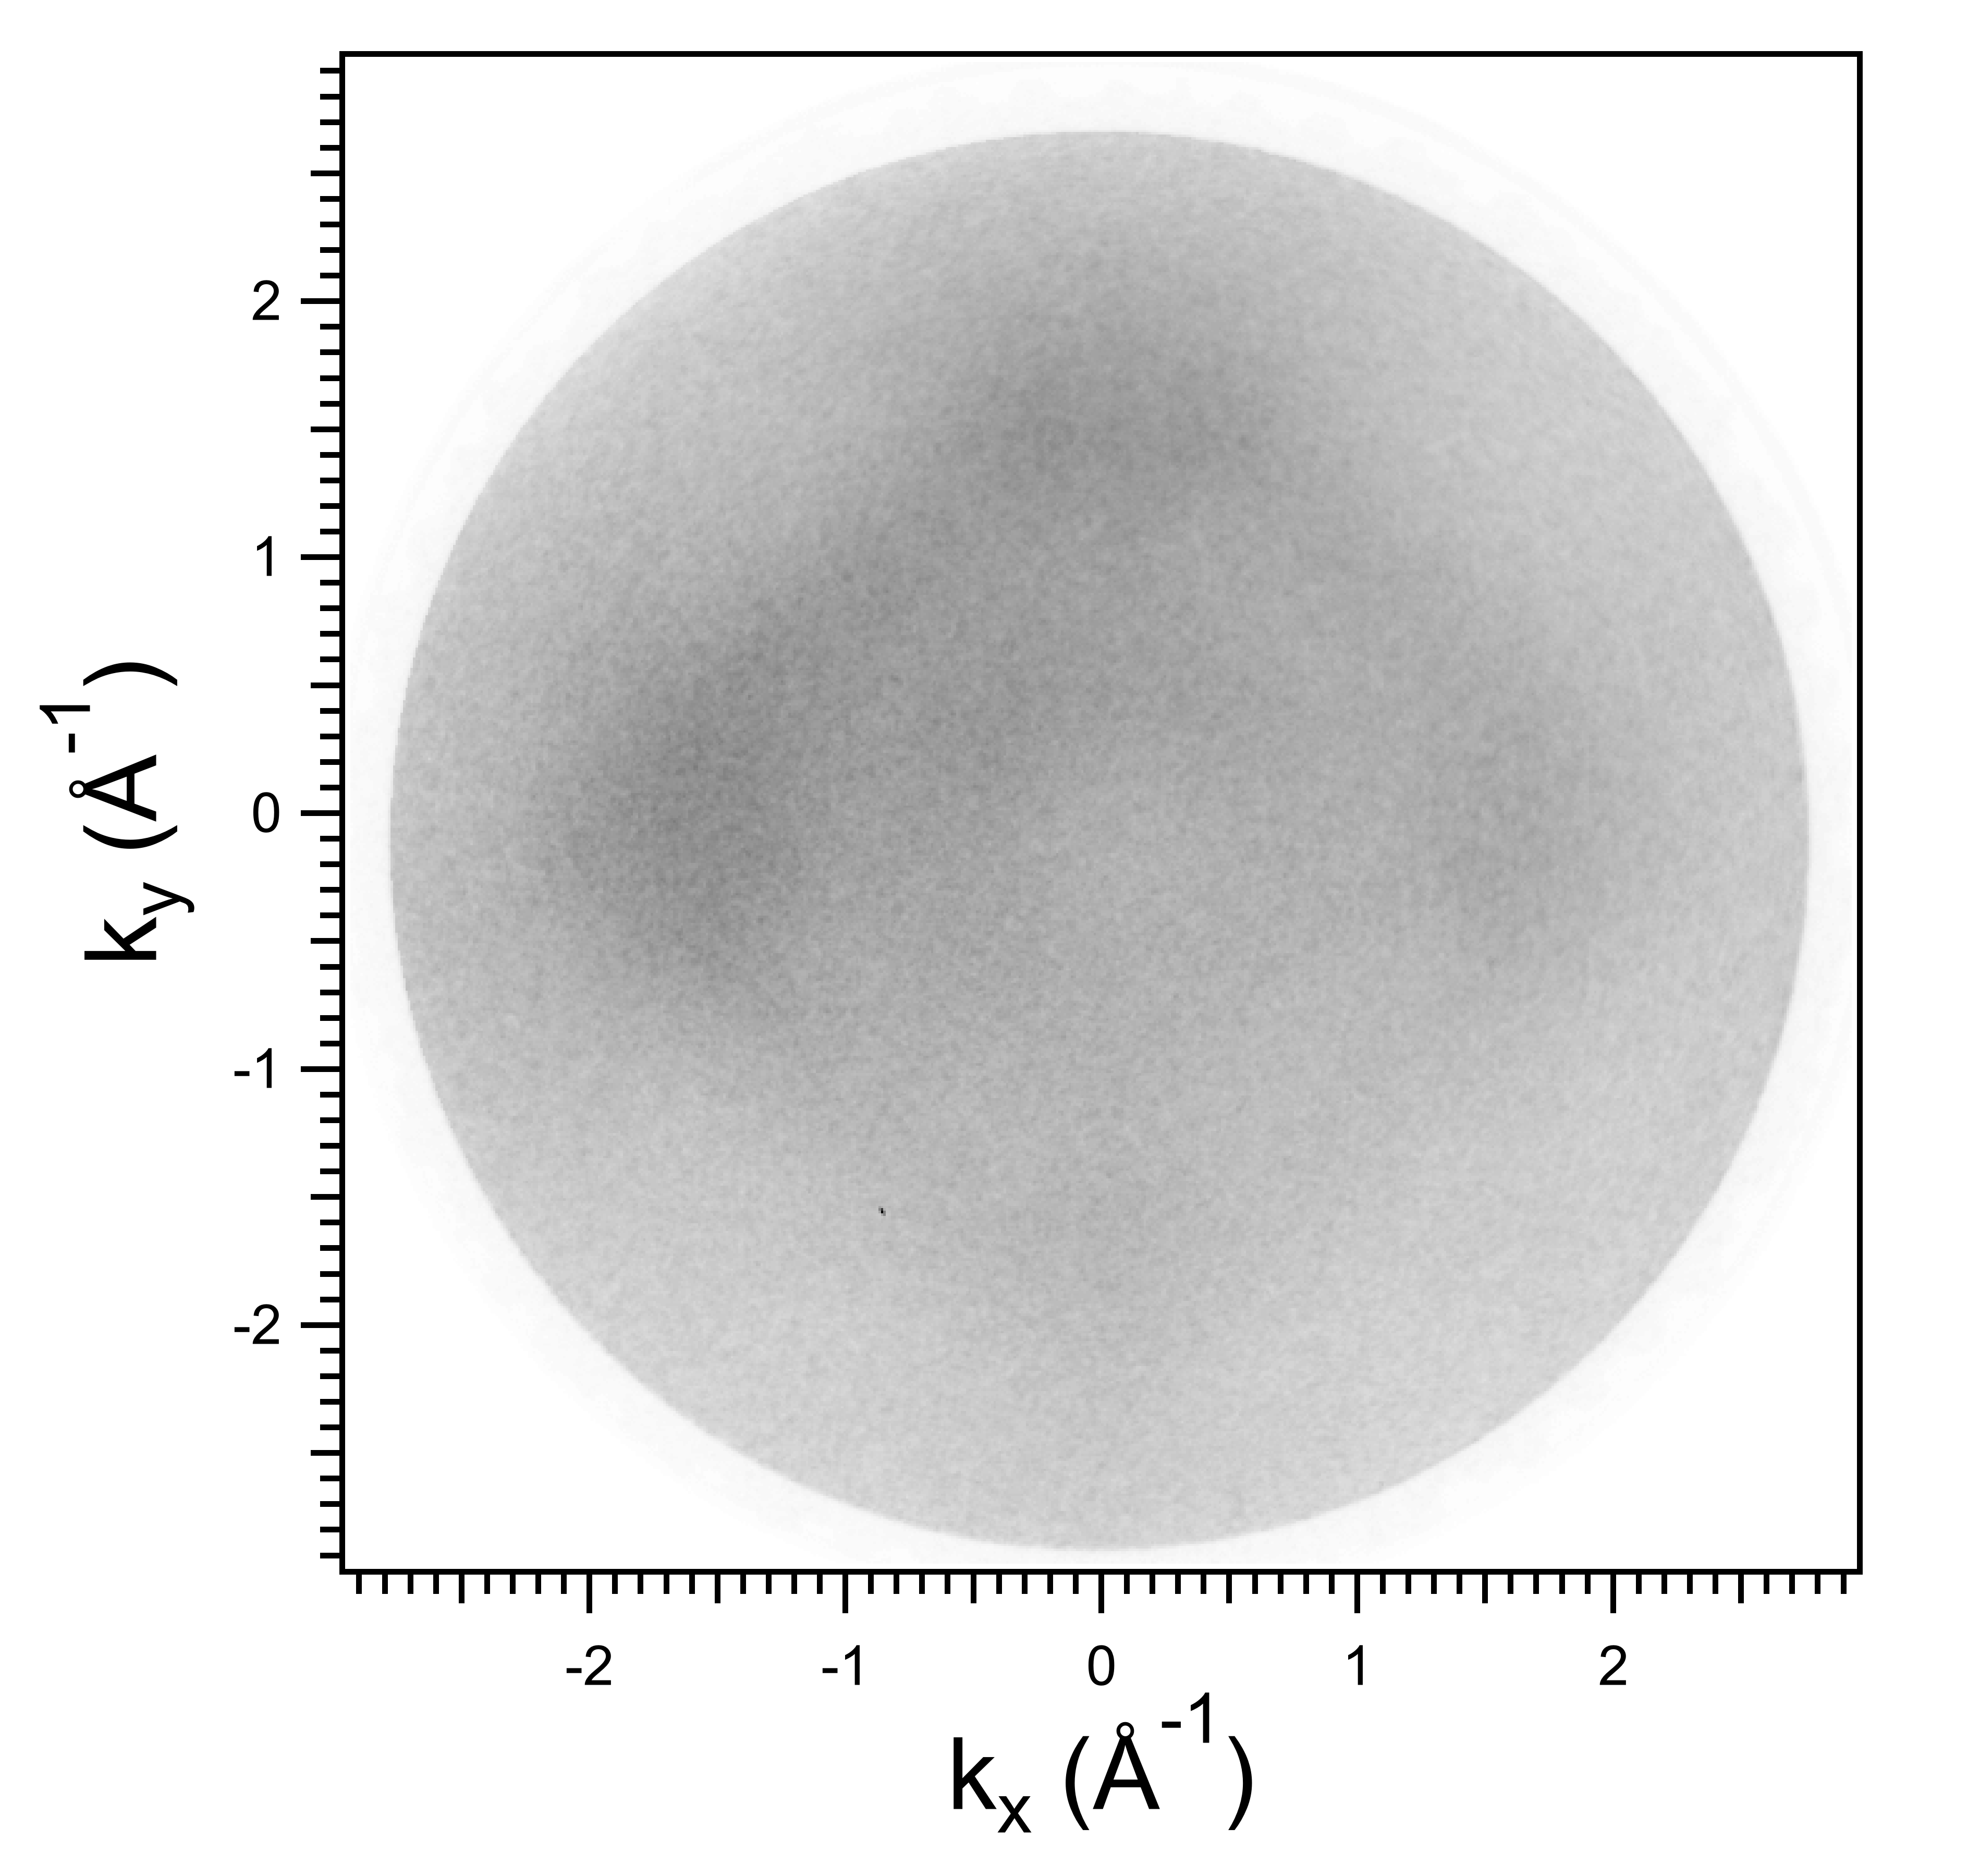
\includegraphics[height=5cm]{./content/pictures/FeO+5A/FeO_5A_32_15eV.png}
                        \subcaption{Das Bild für eine kinetische Energie von \SI{32.15}{\electronvolt}.}
                    \end{subfigure}
                    \begin{subfigure}[t]{0.48\textwidth}
                        \centering
                        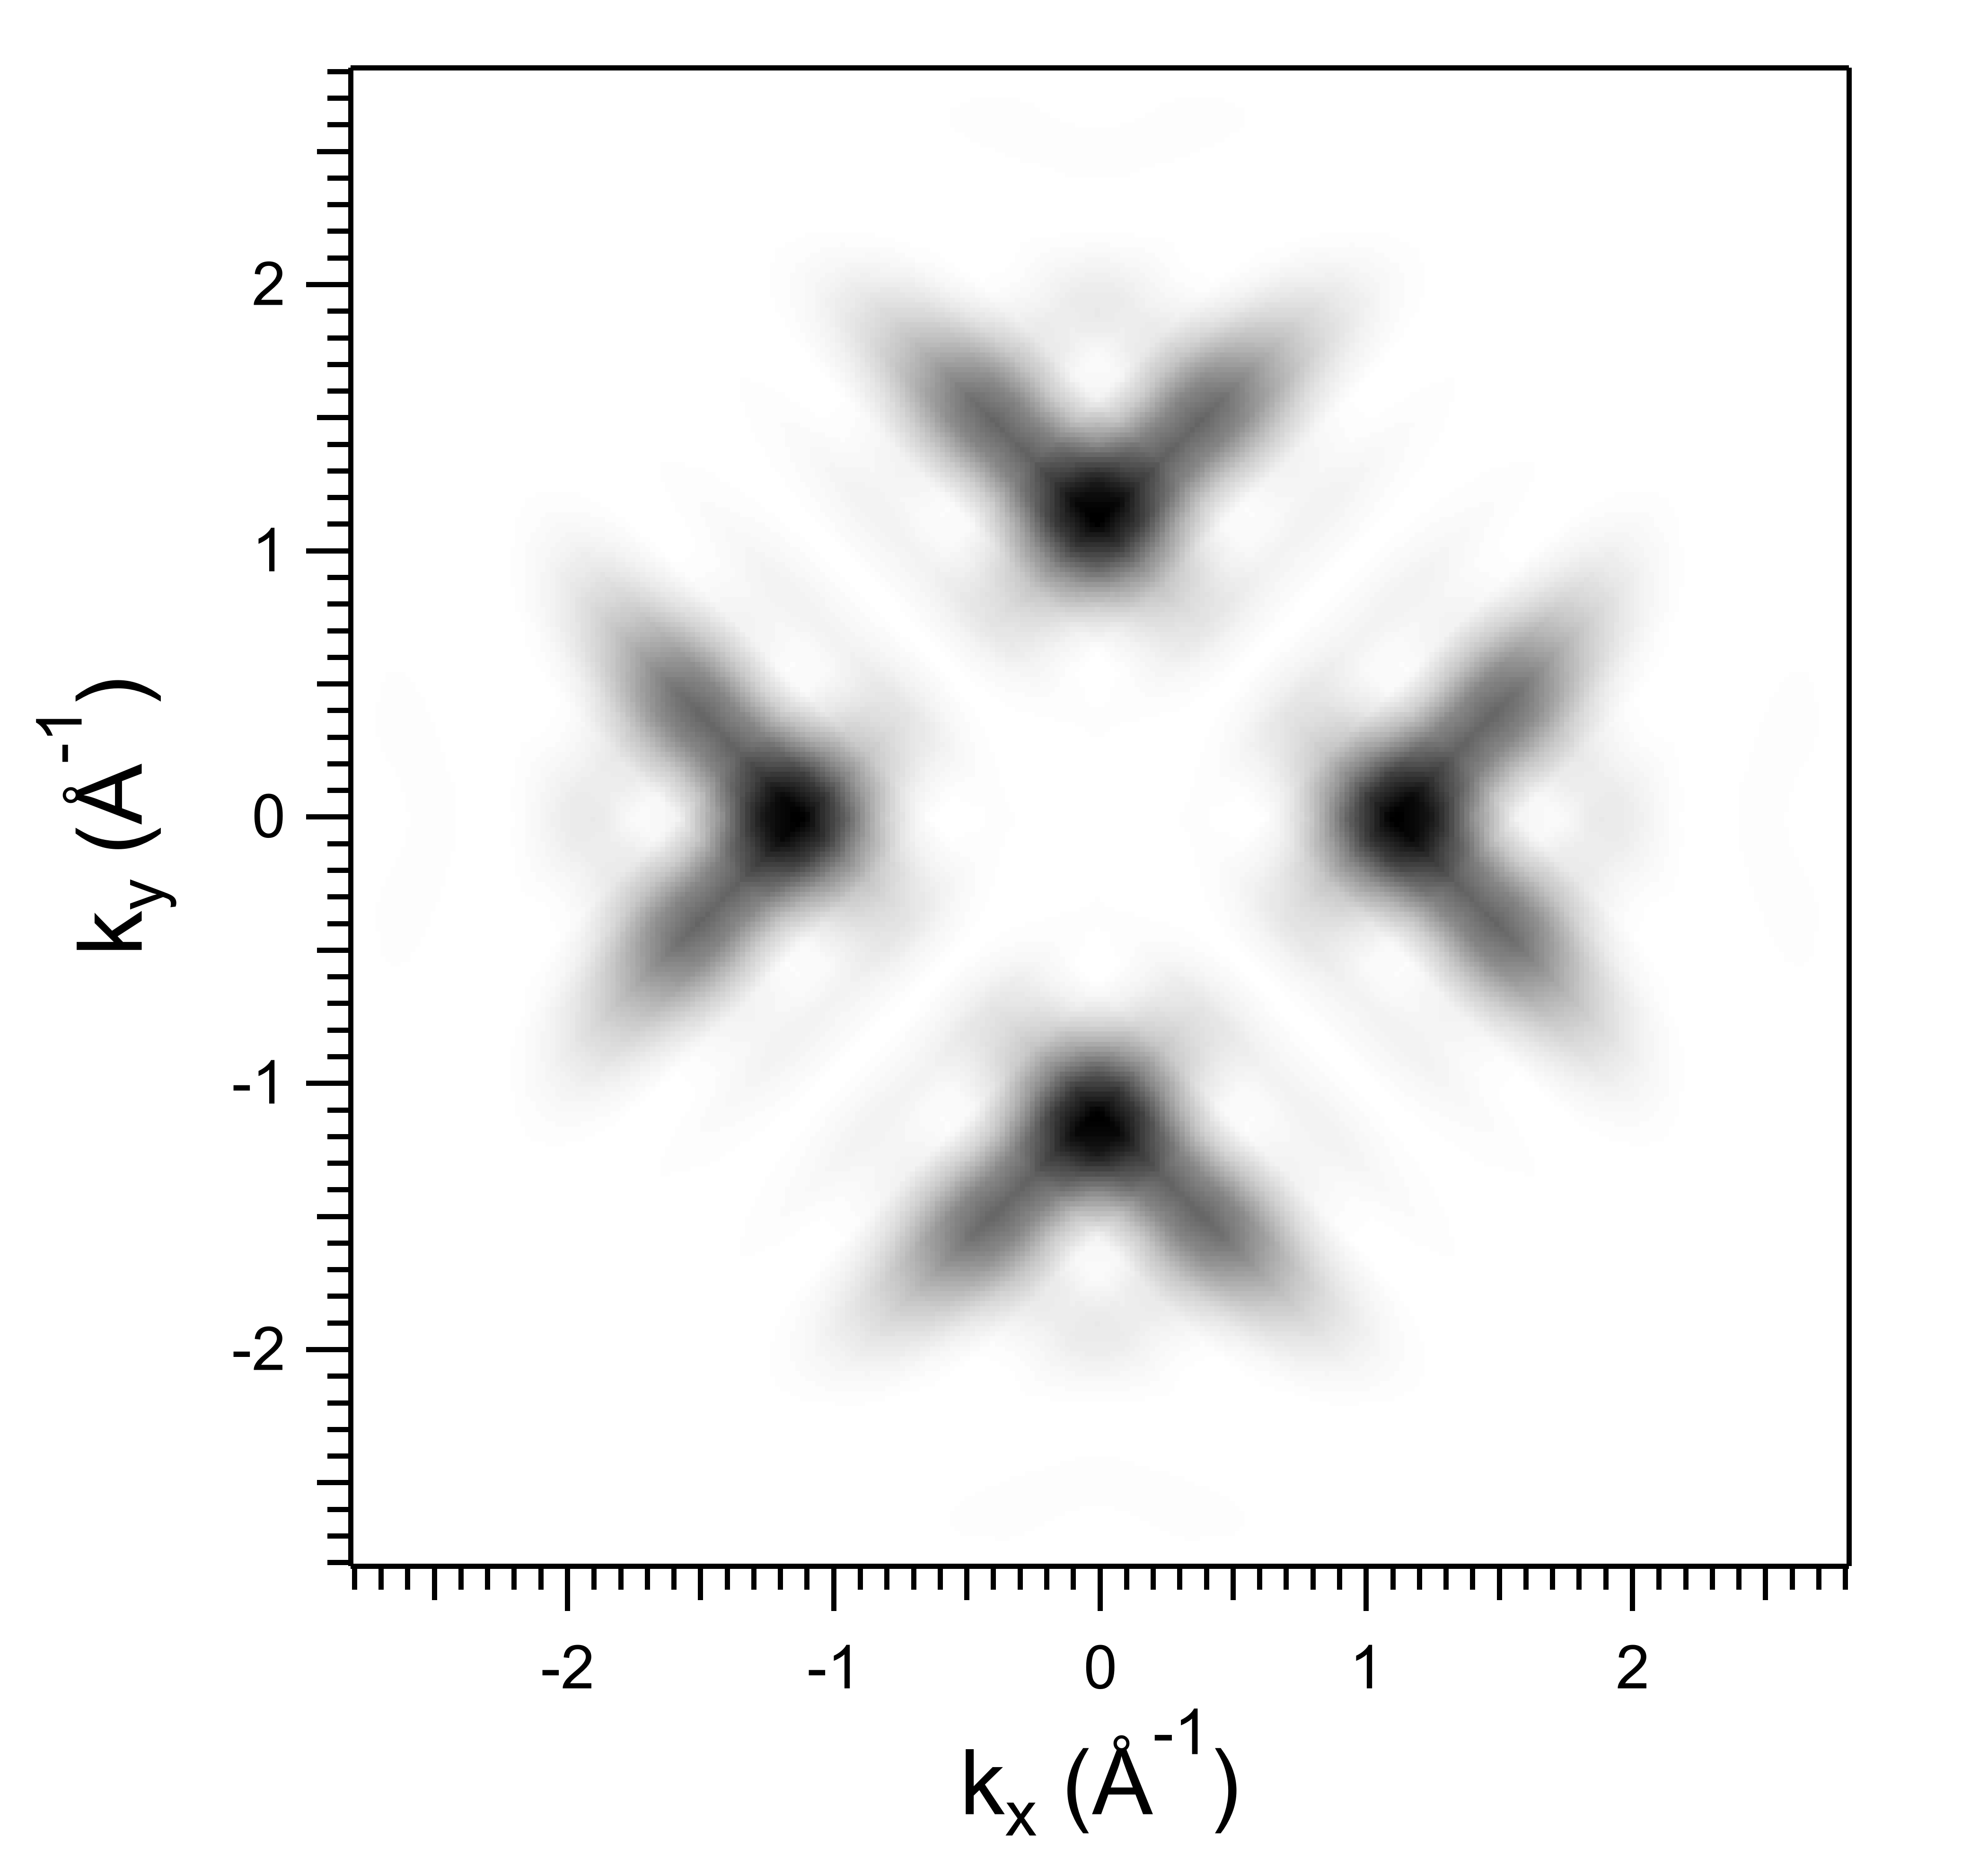
\includegraphics[height=5cm]{./content/pictures/FeO+5A/MO_HOMO1_RT_RT.png}
                        \subcaption{Das HOMO-1 mit Symmetrisierung zweier um \SI{90}{\degree} verdrehten Übergitter.}
                    \end{subfigure}
                    \caption{Vergleich der gemessenen Intensitätsverteilung mit der des symmetrisierten HOMO-1.}
                    \label{fig:FeO5A3}
                \end{figure}
                \begin{figure}
                    \centering
                    \begin{subfigure}[t]{0.48\textwidth}
                        \centering
                        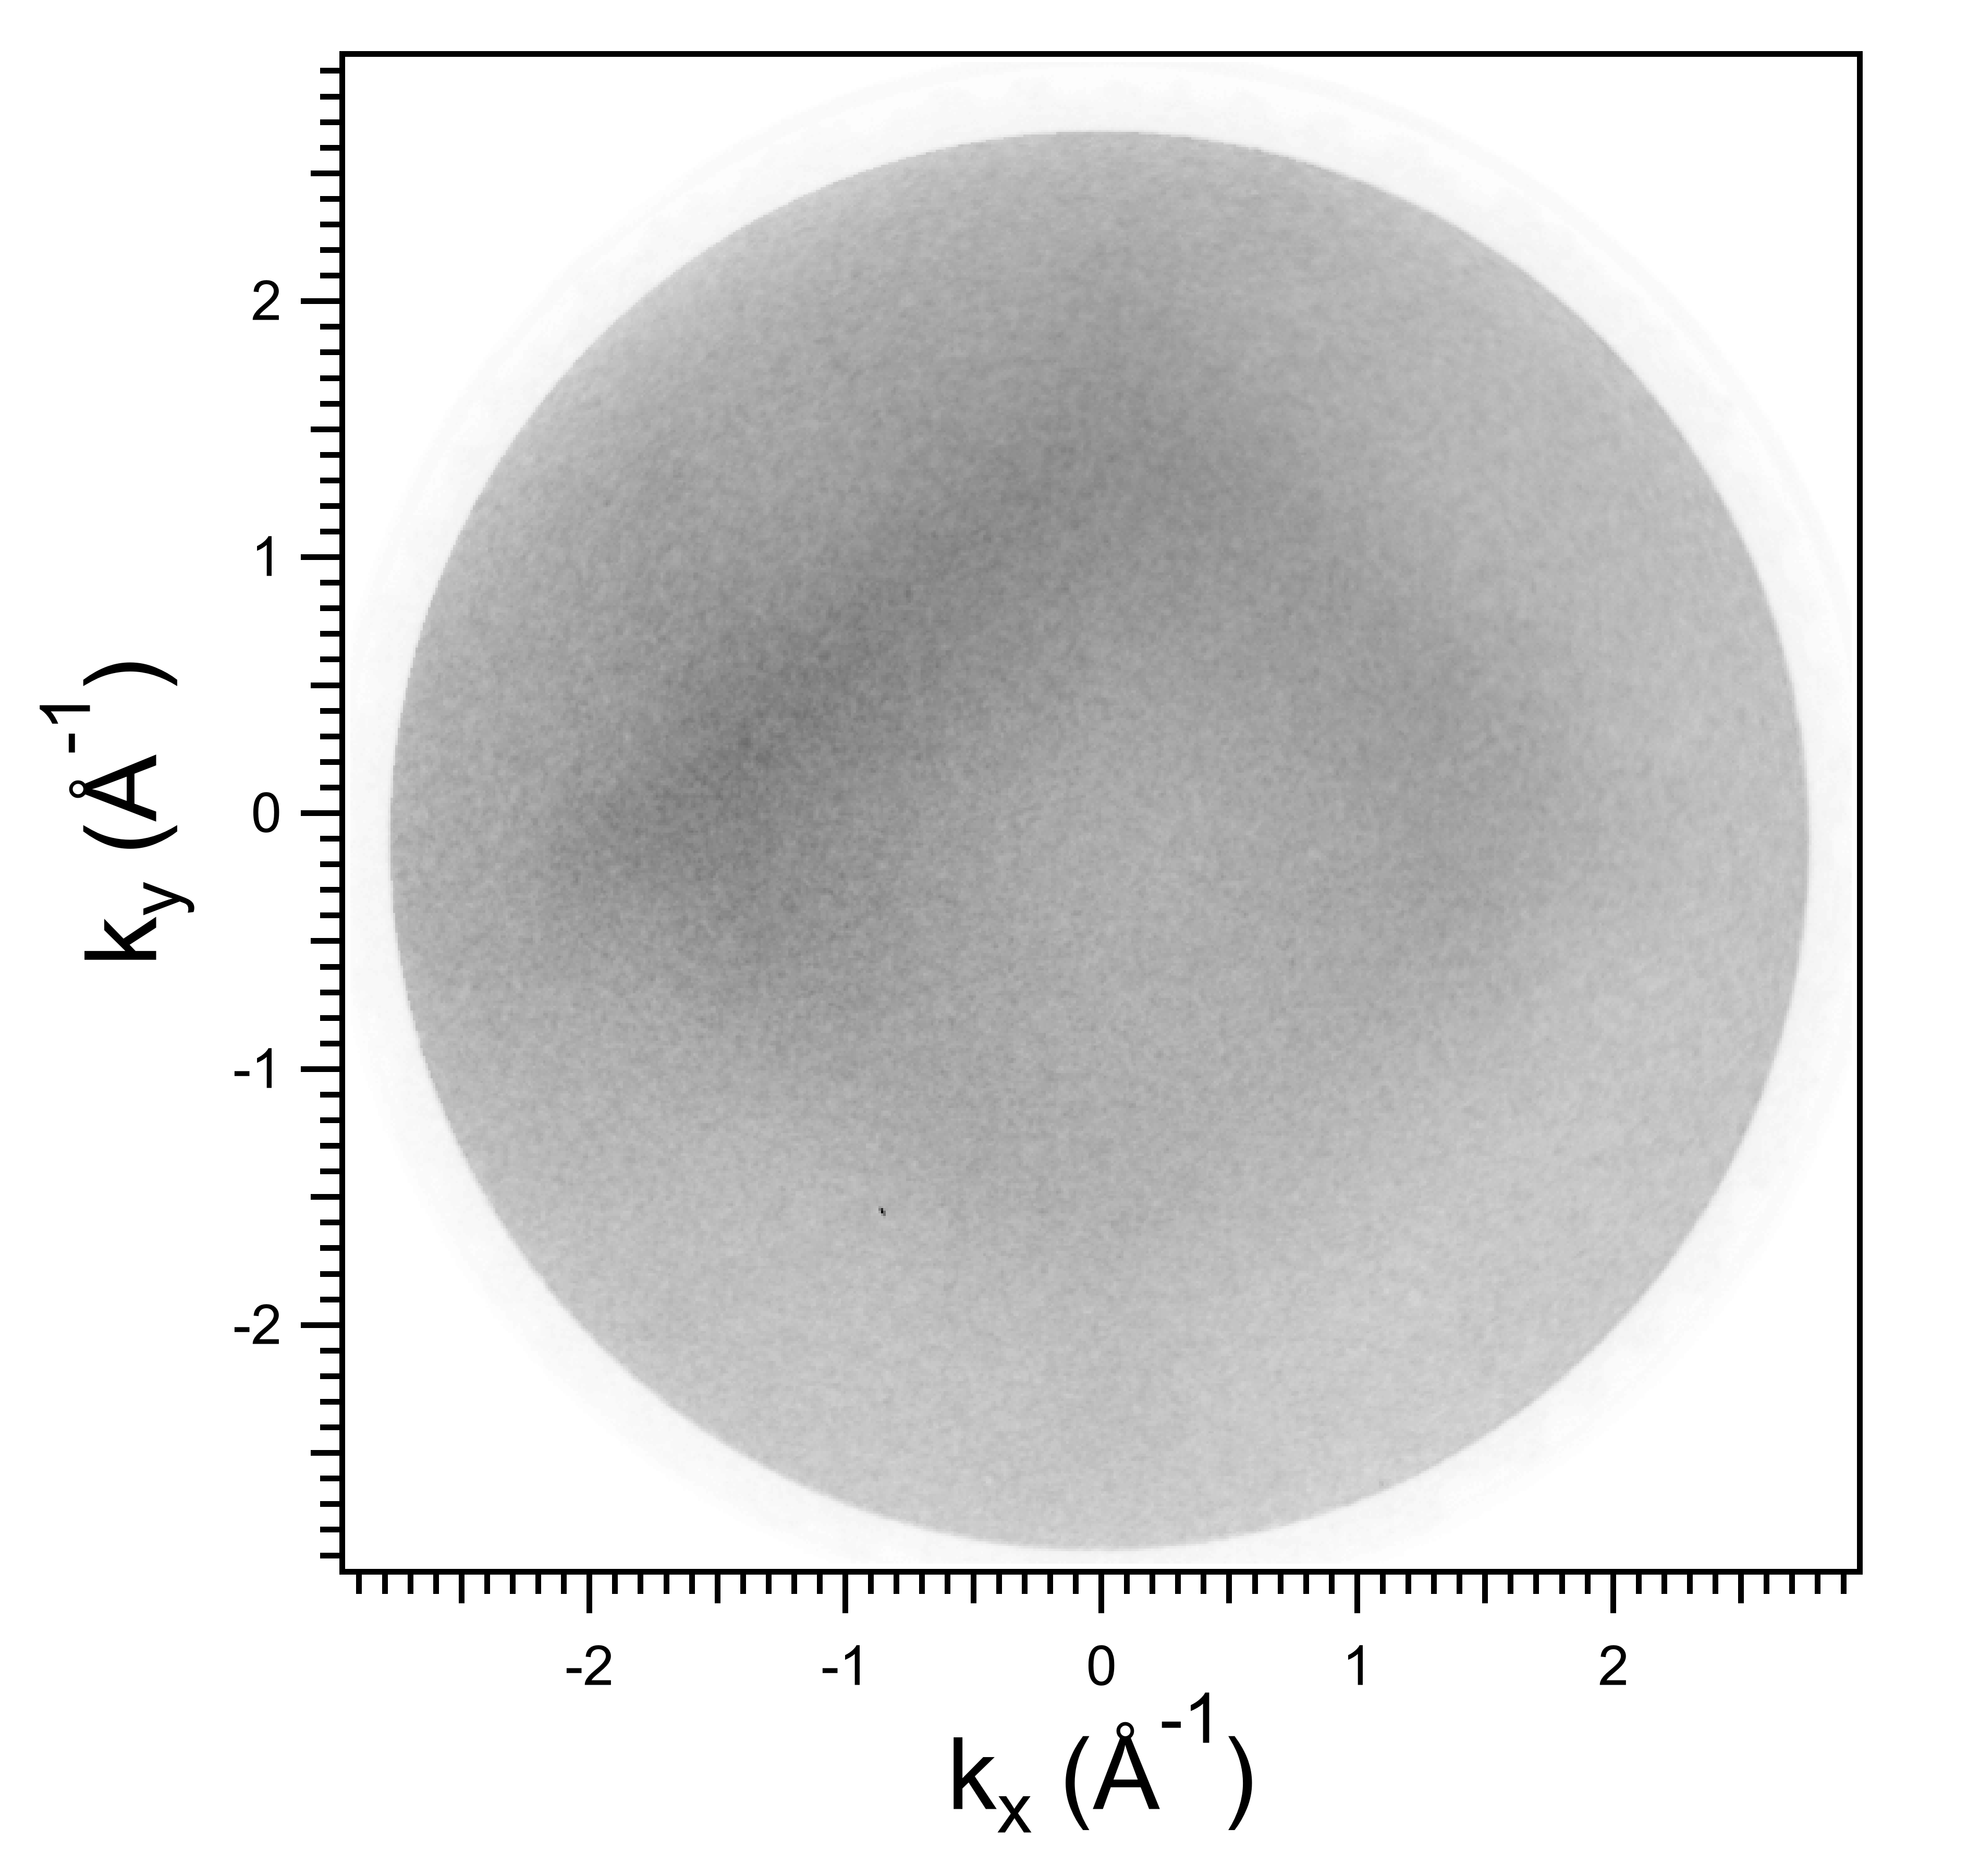
\includegraphics[height=5cm]{./content/pictures/FeO+5A/FeO_5A_30_95eV.png}
                        \subcaption{Das Bild für eine kinetische Energie von \SI{30.95}{\electronvolt}.}
                    \end{subfigure}
                    \begin{subfigure}[t]{0.48\textwidth}
                        \centering
                        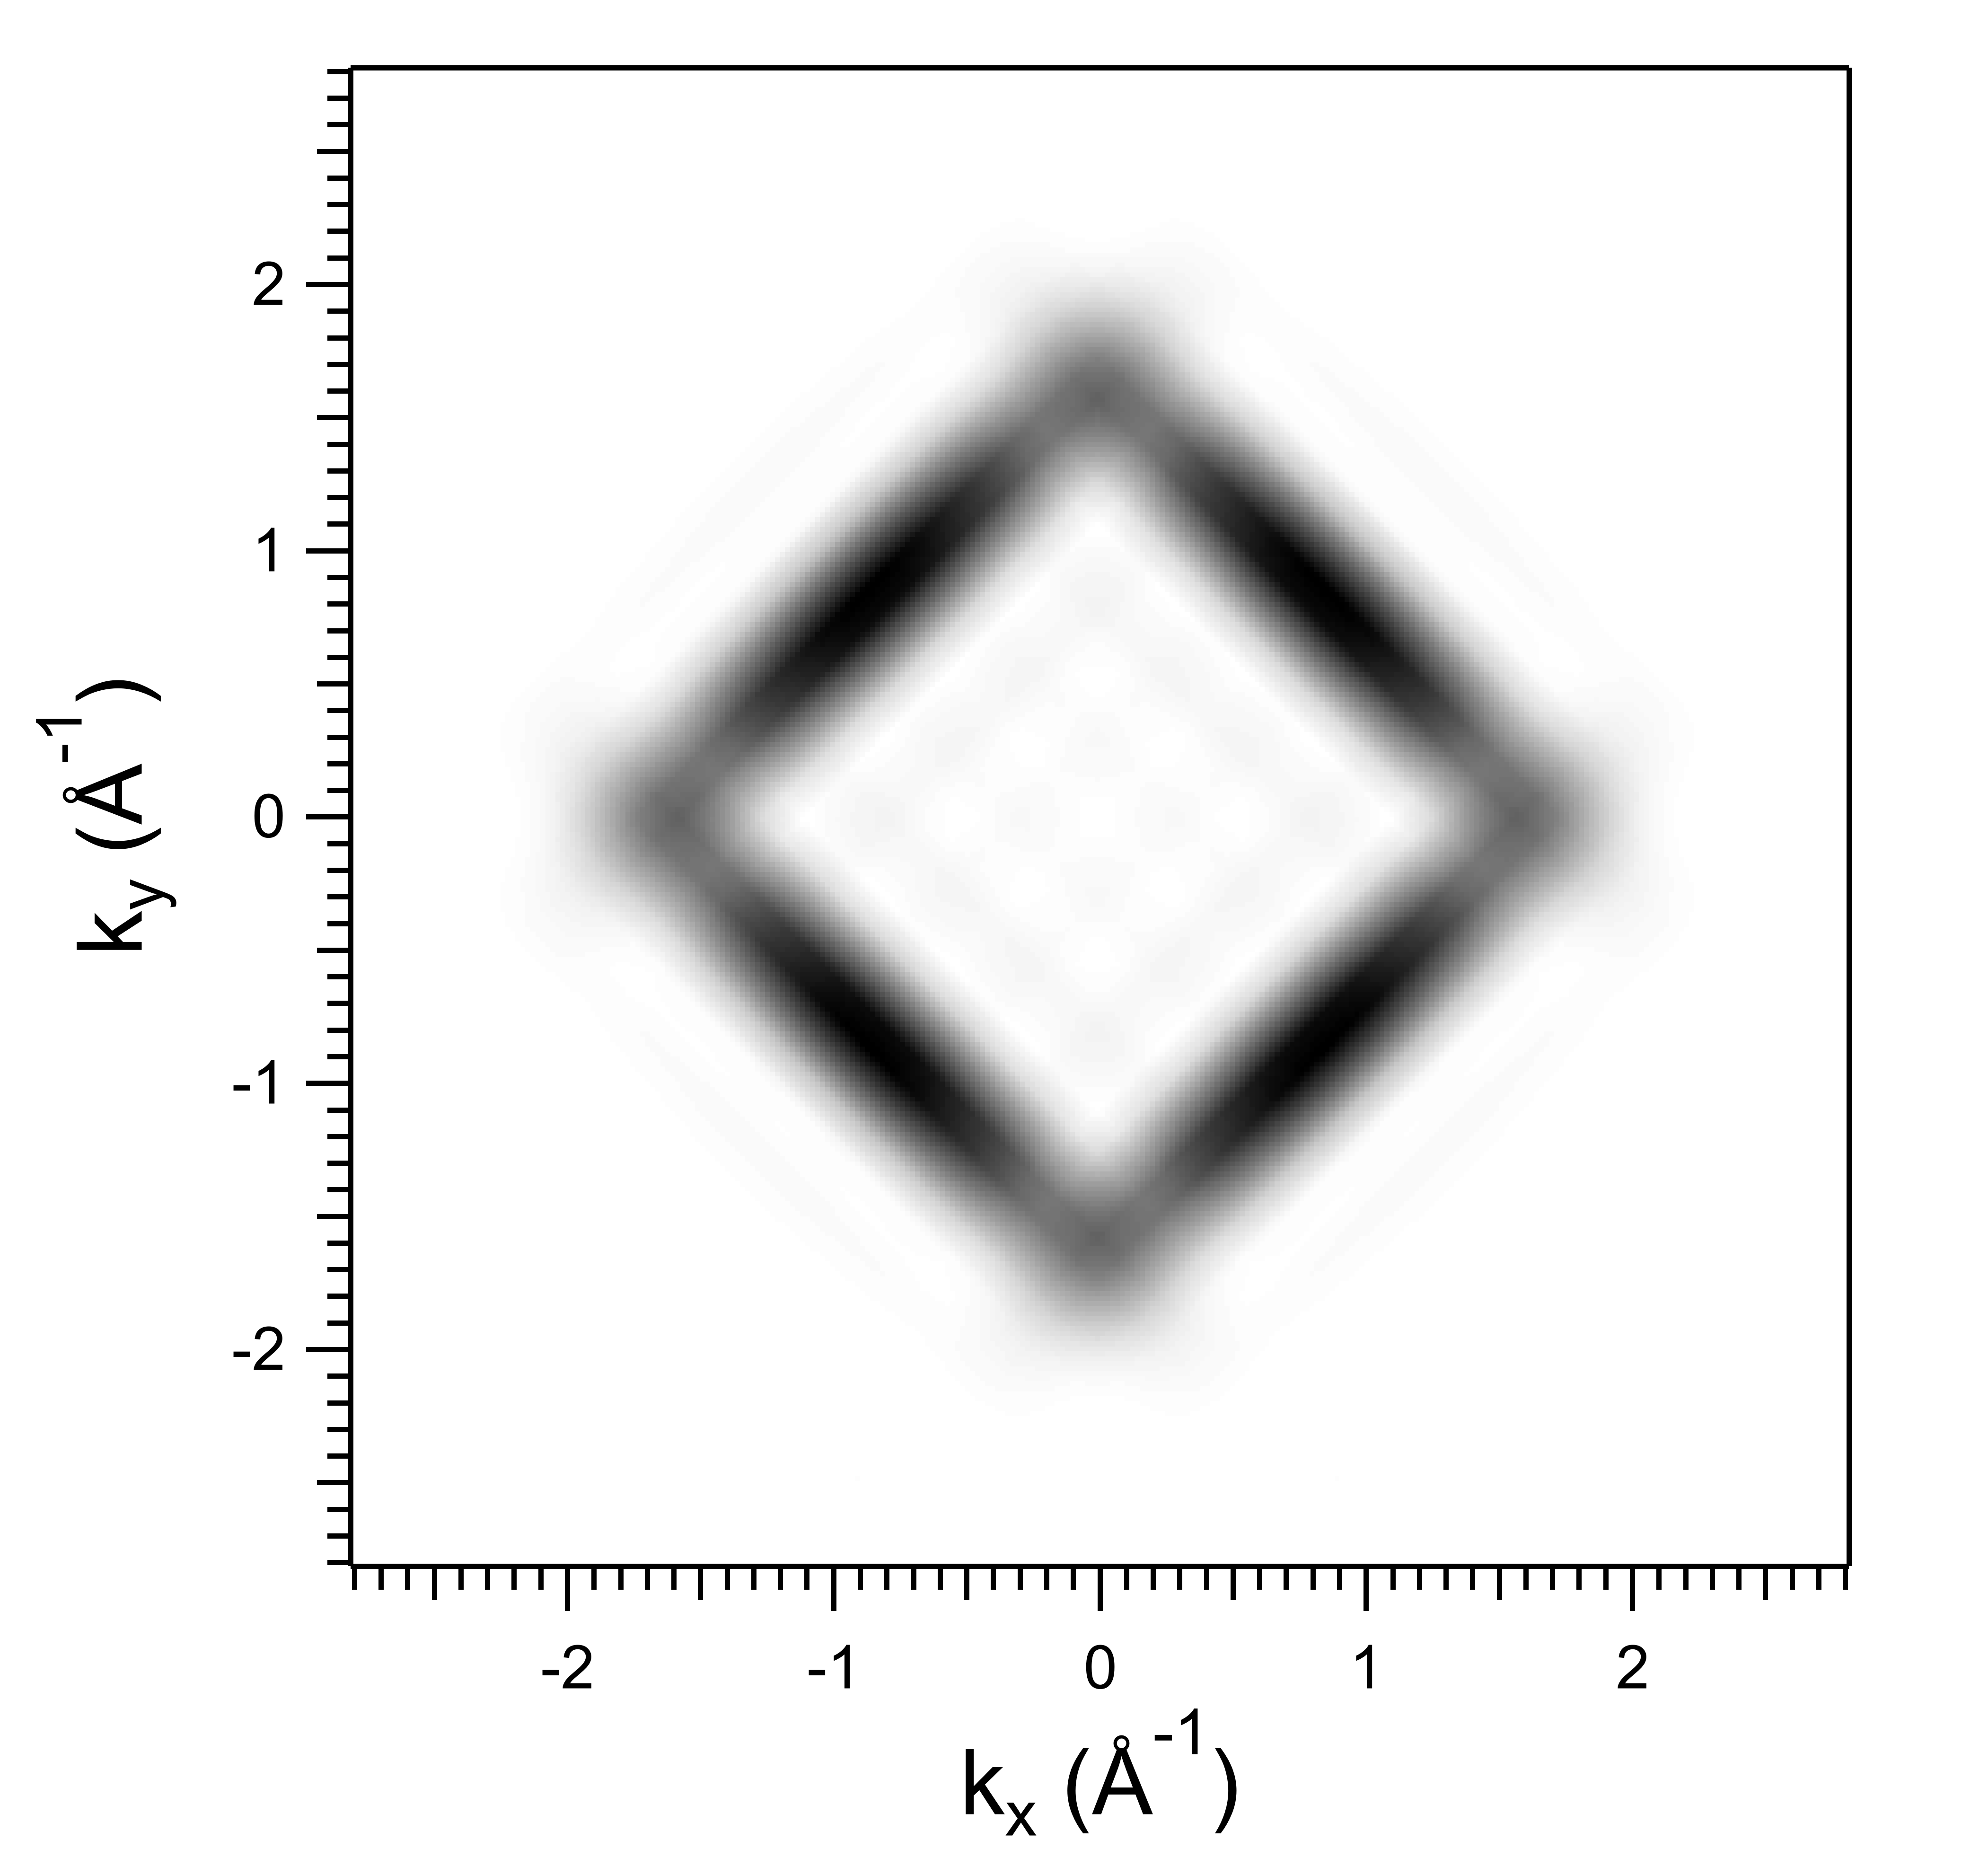
\includegraphics[height=5cm]{./content/pictures/FeO+5A/MO_HOMO2_RT_RT.png}
                        \subcaption{Das HOMO-2 mit Symmetrisierung zweier um \SI{90}{\degree} verdrehten Übergitter.}
                    \end{subfigure}
                    \caption{Vergleich der gemessenen Intensitätsverteilung mit der des symmetrisierten HOMO-2.}
                    \label{fig:FeO5A4}
                \end{figure}

                \begin{itemize}
                    \item Wie liegen die Moleküle zur Substart Achse
                    \item Chemisorption wegen dem besetzten LUMO
                \end{itemize}

